\documentclass{article}

\usepackage{amsmath, amssymb, amsthm}
\usepackage[margin=0.6in]{geometry}
\usepackage[utf8]{inputenc}
\usepackage{hyperref}
\usepackage{graphicx}
\usepackage{pgf}
\graphicspath{{Images/}}
\DeclareUnicodeCharacter{2212}{-}

\hypersetup{
    colorlinks=true,
    urlcolor=blue,
}

\title{Forecasting Stock Price Using Sentiment Analysis and LSTM Networks}
\author{Blake Hillier, Grace Li, Joe Puhalla}
\date{March 31, 2020}

\begin{document}
\maketitle

\section{Overview}
Forecasting stock prices is a widely known problem many people have attempted to solve through various models. A common approach is to use only numerical data to predict tomorrow's price. However, investors often use the news about the company's decisions, the public's attitude towards the company, and the state of the economy when developing trading strategies. In this paper, we propose a model using macro-economic variables to predict the future price of a stock, one of which is statements from the Federal Reserve about decisions on economic policies. Our model is comprised of XLNet to perform sentiment analysis on one macro-economic variable and an LSTM Neural Network to combine all the variables while capturing the effect time has on the future stock price. In this paper we first explain the ideas behind XLNet and LSTM Neural Networks. We then explain our implementation of XLNet and LSTM and calculate their mean squared error (MSE) using appropriate subsets of our data. Finally, we explain how we use them together to forecast the stock price and calculate the entire models MSE before making some concluding remarks.

\section{XLNet}
XLNet is an autoregressive pretraining approach for NLP models. Pretraining a model is used to teach a model a broad field before being applied to a specific problem. This allows it to pick up potential nuances within the data and then apply this knowledge to better understand the specific problem. It also allows copies of the same model to be fine tuned to different problems, decreasing the total learning time. Autoregressive pretraining approaches create a conditional probability distribution based on the likelyhood function \begin{equation*}
    p(x)=\prod_{t=1}^{T}p(x_{t}|x_{<t})
\end{equation*} which only sees the relationship between previous text (it can also be modified to only see the relationship between text after the word). This is problematic since most words derive their meaning from context at both the beginning and the end of a sentence. XLNet solves this problem by calculating a distribution based on all the other text in the word by maximizing \begin{equation*}
    \max_{\theta}E_{z\sim Z_{T}}\left[\sum_{t=1}^{T}\log p_{\theta}(x_{z_{t}}|x_{z<t})\right]=E_{z\sim Z_{T}}\left[\sum_{t=1}^{T}\log\frac{e^{g_{\theta}(x_{z<t,z_{t}})l(x_{t}})}{\sum_{x^{'}}e^{g_{\theta}(x_{z<t,z_{t}})l(x^{'})}}\right]
\end{equation*} where $Z_{T}$ is the set of all permutations of text of length $T$, $z \in Z_{T}, x_{z<t}$ is the sequence of text from 1 to $t−1$, and $g_{\theta}$ transforms $x$ to a sequence of hidden words with the first $t-1$ set of words as additional information. They note the permutations don’t affect the actual order of the text sequence, just the factorization of the likelihood function. Because this is based on the likelihood function, it removes the idea each hidden text is independent of the others while still maintaining the benefits through encoding due to  $g_{\theta}$. In order for  $g_{\theta}$ to accomplish this, they split it into two different transforms: the query $g_{\theta}$ which looks at the first $t-1$ words in the permuted order to predict the  $t^{th}$ word, and the content  $h_{\theta}$ which simply encodes the first t words in the permuted order. The one downside to this model is the complexity of the optimization leading to a slower convergence. To reduce this problem, they adjust the equation to \begin{equation*}
    \max_{\theta}E_{z \sim Z_{T}}\left[\log_{p_{\theta}}(x_{z>c}|x_{z\leq t})\right]=E_{z\sim Z_{T}}\left[\sum_{t=c+1}^{|z|}\log p_{\theta}(x_{z_{t}}|x_{z<t})\right]
\end{equation*}
which changes the model to only predict the last $T - c$ words in the permutation order, where $c \approx \frac{T(1+K)}{K}$
for some parameter $K$.

\section{LSTM}

In this paper, the LSTM neural network is uesed to predict the stock price, the input data is the historical stock price and sentiment analysis results. Here, the sentiment based LSTM neural network (named sentiment-LSTM) is aimed to minimize the following loss function:

$$ \ell = min \sum_{t=p+1}^{p+T} \bigg\| X_{t} - \hat{X_{t}} \bigg\|_{2}^{2} $$

Where $T$ denotes the number of prediction time slots, i.e, $t$ = 1, ..., $p$ are the observations (training input data), $t = p+1, ..., p+T$ are the predicts (training output data); and $\hat{X}_{t}$ is given as following:

$$\hat{X}_t = \alpha X_{t}^{A} + \lambda S_{t}^{A} + c = \alpha X_{t}^{A} + \lambda f_{2}\underbrace{((S_{t-i})_{i=1}^{p})}_\text{Sentiment}+c$$

\begin{figure}[htp]
    \centering
    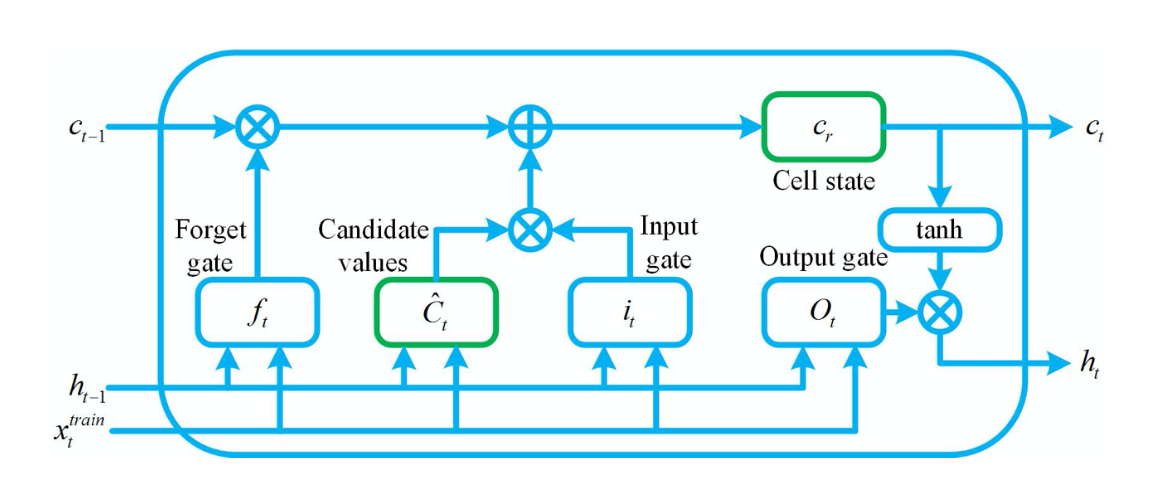
\includegraphics[width=7cm]{LSTM.png}
    \caption{LSTM Procedure}
    \label{fig:LSTM}
\end{figure}

Denote Formula as the training input data. Figure 1 shows the LSTM's structure network, which comprises one or more hidden layers, an output layer and an input layer. LSTM networks’ main advantage is that the hidden layer comprises memory cells. Each memory cell recurrently has a core self-connected linear unit called “ Constant Error Carousel, which provides short-term memory storage and has three gates:

\textbf{Input gate}, which controls the information from a new input to the memory cell, is given by

$$i_{t} = \sigma (W_{i} \times [h_{t-1}, \chi_{t}^{train}] + b_{i})$$
$$\hat{c_{t}} = tanh(W_{c} \times [h_{t-1}, \chi_{t}^{train}] + b_{c} )$$

$h_{t-1}$ is the hidden state at the time step $t-1;i_{t}$ is the output of the input gate layer at the time step $t; \hat{c_{t}} $ is the candidate value to be added to the output at the time step $t; b_{i}$ and $b_{c}$ are biases of the input gate layer and the candidate value computation, respectively; $W_{i}$ and $W_{c}$ are weights of the input gate and the candidate value computation respectively; and $\sigma (x) = 1/(1+e^{-x})$ is the pointwise nonlinear activation function.

\textbf{Forget gate}, which controls the limit up to which a value is saved in the memory, is given by
$$f(t) = \sigma (W_{f} \times [h_{t-1}, \chi_{t}^{train}]+b_{f})$$
where $f_{t}$ is the forget state at the time step $t, W_{f}$ is the weight of the forget gate; and $b_{f}$ is the bias of the forget gate.

\textbf{Output gate}, which controls the information output from the memory cell, is given by

$$ c_{t} = f_{t} \times c_{t-1} + i_{t} \times \hat{c_{t}}$$
$$o_{t} = \sigma (W_{o} \times [h_{t-1}, \chi_{t}^{train}] + b_{o})$$
$$h_{t} = o_{t} \times tanh(c_{t})$$

where new cell state $c_{t}$ are calculated based on the results of the previous two steps; $o_{t}$ is the output at the time step $t; W_{o}$ is the weight of the output gate; and $b_{o}$ is the bias of the out put gate. \\

\section{Experiment}
Because our model has multiple core algorithms, we need to calibrate each main component individually as well as when they are all together to ensure we are obtaining an optimal accuracy. This section will discuss the data we use, how each algorithm performs on their own, and how they perform when put together.
\subsection{Data}
Our data consisted of macroeconomic data and the previous stock priced. The macroeconomic data consisted of the quarterly GDP, monthly CPI, monthly unemployment rate, monthly inflation rate, the ten-year treasury rate, the 1 year LIBOR daily, and the statements from the Federal Reserve. All the data ranges from the beginning of the year 2000 to the end of 2014. Since our stock is daily data, all previous data were duplicated into daily data and aligned with the stock information.
\subsection{Sentiment Analysis}
We used pytorch's implementation of XLNet-base for our model. Sentiment was assigned to the Fed's Statements by looking at the percent change of the UNH stock. If the stock increased, the sentiment was positive, and negative otherwise. We then tested the accuracy of the XLNet by randomly selecting $80\%$ of the data to train, and the remaining $20\%$ to test. This was done using a GPU on Google's Colab. We had to carefully select our batch size, maximum statement length, and epoch combinations carefully due to memory constraints. This posed an interesting problem for us since a larger maximum statement size allows more of the Fed's statement to be considered for sentiment, but requires a smaller batch size resulting in severe over fitting. A smaller statement size reduces the amount of information available, but allows a bigger batch size leading to better generalizations. After some testing we found a maximum statement length of 128, batch size of 24, and 10 epochs produced the best accuracy of $77.1\%$.
\subsection{LSTM Stock Prediction}
\begin{figure}
\begin{minipage}{0.5\textwidth}
    \centering
    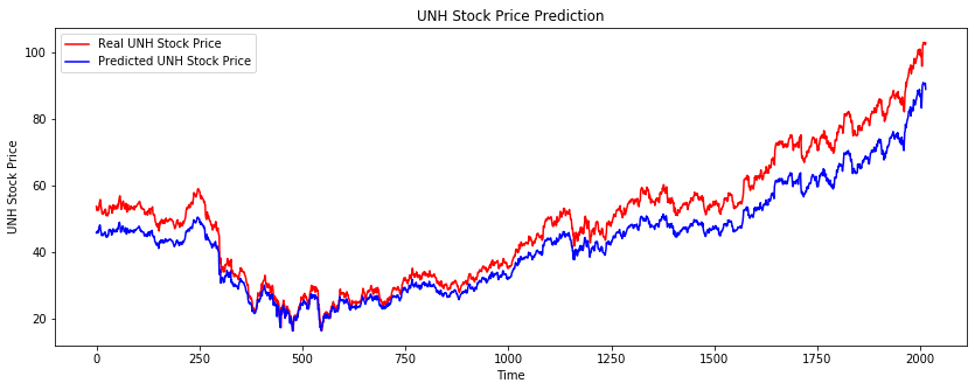
\includegraphics[width=9cm]{LSTMResult.png}
    \caption{Predicted vs. Actual Stock Price}
    \label{fig:LSTMForecast}
\end{minipage}
\begin{minipage}{0.5\textwidth}
    \centering
    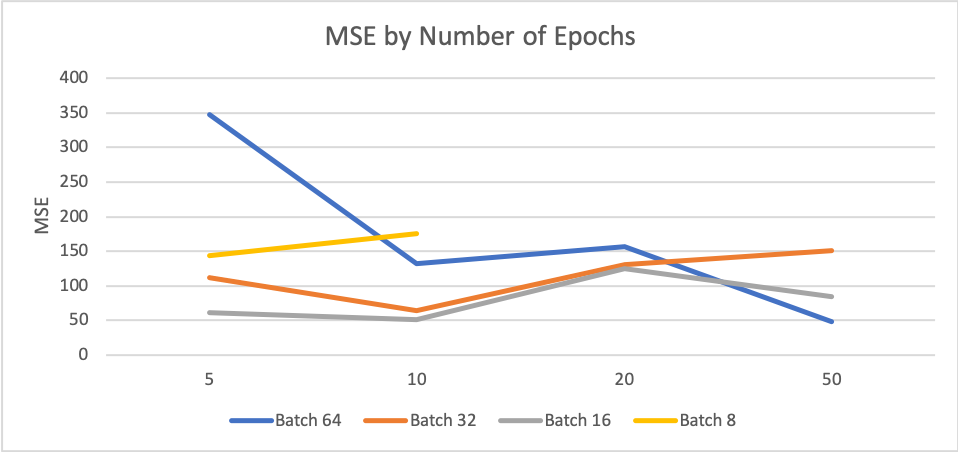
\includegraphics[width=9cm]{LSTMMSE.png}
    \caption{MSE by Number of Epochs}
    \label{fig:LSTMResult}
\end{minipage}
\end{figure}

The LSTM network we use includes four layers each with a dropout rate of twenty percent. The layers are of size $256,128,64,32$ and then the final layer. We sampled through several activation functions, starting with linear activation, and determined the ReLu activation to provide the best accuracy of the model. In order to determine the accuracy of the model, we plot both the predicted and actual stock price values of UNH. We then determine the mean squared error between the predicted and actual prices. We sampled across several amounts of epochs $(5,10,20,50)$ and batch sizes $(8,16,32, 64)$ in order to determine the best architecture for the model. For simplicity purposes, we used the already given ‘adam’ optimizer. Our feature set for the model were daily measures of price, GDP, CPI, inflation, unemployment, LIBOR, and the 10-year treasury yield. GDP data was given quarterly and thus had to be converted to daily data. In addition, CPI, inflation, and unemployment were given as monthly data and were converted to daily data. Our train and test data were split 50-50.
With a batch size of 8, the 20 and 50 epoch sized networks caused memory issues and thus were unable to be completed. A batch size of 64, and 50 epochs yielded the lowest MSE among all models $(\ref{fig:LSTMForecast})$. More tests need to be conducted in order to determine the most accurate model. Furthermore, the number of layers needs to be varied as well as the optimizer used. Tests need to be done to determine which features contribute the most to the predicting power of our model. Sentiment scores of the FOMC transcripts also need to be added as features of the model. The preliminary results provide for a proof of concept for our model and give promise to further tests with more features.  
\subsection{XLNet and LSTM}
Using the optimal model parameters through the previous sections, we created a pipeline using both models. We first trained the XLNet on the entire text data, and then predicted the sentiment on the same dataset. This was then merged with the input data for the LSTM, and was trained using a portion of the stock data. Once trained, we validated it with the last 2014 data points to obtain the MSE: 25.226. This is lower than our previous tests with the LSTM, showing the capability of XLNet improving our forecasting accuracy. Figure $\ref{fig:XLNetLSTMForcast}$ shows our test case after training with XLNet and the LSTM model. 
\begin{figure}
    \centering
    \scalebox{0.5}{%% Creator: Matplotlib, PGF backend
%%
%% To include the figure in your LaTeX document, write
%%   \input{<filename>.pgf}
%%
%% Make sure the required packages are loaded in your preamble
%%   \usepackage{pgf}
%%
%% and, on pdftex
%%   \usepackage[utf8]{inputenc}\DeclareUnicodeCharacter{2212}{-}
%%
%% or, on luatex and xetex
%%   \usepackage{unicode-math}
%%
%% Figures using additional raster images can only be included by \input if
%% they are in the same directory as the main LaTeX file. For loading figures
%% from other directories you can use the `import` package
%%   \usepackage{import}
%%
%% and then include the figures with
%%   \import{<path to file>}{<filename>.pgf}
%%
%% Matplotlib used the following preamble
%%   \usepackage{fontspec}
%%   \setmainfont{DejaVuSerif.ttf}[Path=/usr/local/lib/python3.6/dist-packages/matplotlib/mpl-data/fonts/ttf/]
%%   \setsansfont{DejaVuSans.ttf}[Path=/usr/local/lib/python3.6/dist-packages/matplotlib/mpl-data/fonts/ttf/]
%%   \setmonofont{DejaVuSansMono.ttf}[Path=/usr/local/lib/python3.6/dist-packages/matplotlib/mpl-data/fonts/ttf/]
%%
\begingroup%
\makeatletter%
\begin{pgfpicture}%
\pgfpathrectangle{\pgfpointorigin}{\pgfqpoint{14.000000in}{5.000000in}}%
\pgfusepath{use as bounding box, clip}%
\begin{pgfscope}%
\pgfsetbuttcap%
\pgfsetmiterjoin%
\definecolor{currentfill}{rgb}{1.000000,1.000000,1.000000}%
\pgfsetfillcolor{currentfill}%
\pgfsetlinewidth{0.000000pt}%
\definecolor{currentstroke}{rgb}{1.000000,1.000000,1.000000}%
\pgfsetstrokecolor{currentstroke}%
\pgfsetdash{}{0pt}%
\pgfpathmoveto{\pgfqpoint{0.000000in}{0.000000in}}%
\pgfpathlineto{\pgfqpoint{14.000000in}{0.000000in}}%
\pgfpathlineto{\pgfqpoint{14.000000in}{5.000000in}}%
\pgfpathlineto{\pgfqpoint{0.000000in}{5.000000in}}%
\pgfpathclose%
\pgfusepath{fill}%
\end{pgfscope}%
\begin{pgfscope}%
\pgfsetbuttcap%
\pgfsetmiterjoin%
\definecolor{currentfill}{rgb}{1.000000,1.000000,1.000000}%
\pgfsetfillcolor{currentfill}%
\pgfsetlinewidth{0.000000pt}%
\definecolor{currentstroke}{rgb}{0.000000,0.000000,0.000000}%
\pgfsetstrokecolor{currentstroke}%
\pgfsetstrokeopacity{0.000000}%
\pgfsetdash{}{0pt}%
\pgfpathmoveto{\pgfqpoint{1.750000in}{0.550000in}}%
\pgfpathlineto{\pgfqpoint{12.600000in}{0.550000in}}%
\pgfpathlineto{\pgfqpoint{12.600000in}{4.400000in}}%
\pgfpathlineto{\pgfqpoint{1.750000in}{4.400000in}}%
\pgfpathclose%
\pgfusepath{fill}%
\end{pgfscope}%
\begin{pgfscope}%
\pgfsetbuttcap%
\pgfsetroundjoin%
\definecolor{currentfill}{rgb}{0.000000,0.000000,0.000000}%
\pgfsetfillcolor{currentfill}%
\pgfsetlinewidth{0.803000pt}%
\definecolor{currentstroke}{rgb}{0.000000,0.000000,0.000000}%
\pgfsetstrokecolor{currentstroke}%
\pgfsetdash{}{0pt}%
\pgfsys@defobject{currentmarker}{\pgfqpoint{0.000000in}{-0.048611in}}{\pgfqpoint{0.000000in}{0.000000in}}{%
\pgfpathmoveto{\pgfqpoint{0.000000in}{0.000000in}}%
\pgfpathlineto{\pgfqpoint{0.000000in}{-0.048611in}}%
\pgfusepath{stroke,fill}%
}%
\begin{pgfscope}%
\pgfsys@transformshift{2.243182in}{0.550000in}%
\pgfsys@useobject{currentmarker}{}%
\end{pgfscope}%
\end{pgfscope}%
\begin{pgfscope}%
\definecolor{textcolor}{rgb}{0.000000,0.000000,0.000000}%
\pgfsetstrokecolor{textcolor}%
\pgfsetfillcolor{textcolor}%
\pgftext[x=2.243182in,y=0.452778in,,top]{\color{textcolor}\sffamily\fontsize{10.000000}{12.000000}\selectfont 0}%
\end{pgfscope}%
\begin{pgfscope}%
\pgfsetbuttcap%
\pgfsetroundjoin%
\definecolor{currentfill}{rgb}{0.000000,0.000000,0.000000}%
\pgfsetfillcolor{currentfill}%
\pgfsetlinewidth{0.803000pt}%
\definecolor{currentstroke}{rgb}{0.000000,0.000000,0.000000}%
\pgfsetstrokecolor{currentstroke}%
\pgfsetdash{}{0pt}%
\pgfsys@defobject{currentmarker}{\pgfqpoint{0.000000in}{-0.048611in}}{\pgfqpoint{0.000000in}{0.000000in}}{%
\pgfpathmoveto{\pgfqpoint{0.000000in}{0.000000in}}%
\pgfpathlineto{\pgfqpoint{0.000000in}{-0.048611in}}%
\pgfusepath{stroke,fill}%
}%
\begin{pgfscope}%
\pgfsys@transformshift{3.468174in}{0.550000in}%
\pgfsys@useobject{currentmarker}{}%
\end{pgfscope}%
\end{pgfscope}%
\begin{pgfscope}%
\definecolor{textcolor}{rgb}{0.000000,0.000000,0.000000}%
\pgfsetstrokecolor{textcolor}%
\pgfsetfillcolor{textcolor}%
\pgftext[x=3.468174in,y=0.452778in,,top]{\color{textcolor}\sffamily\fontsize{10.000000}{12.000000}\selectfont 250}%
\end{pgfscope}%
\begin{pgfscope}%
\pgfsetbuttcap%
\pgfsetroundjoin%
\definecolor{currentfill}{rgb}{0.000000,0.000000,0.000000}%
\pgfsetfillcolor{currentfill}%
\pgfsetlinewidth{0.803000pt}%
\definecolor{currentstroke}{rgb}{0.000000,0.000000,0.000000}%
\pgfsetstrokecolor{currentstroke}%
\pgfsetdash{}{0pt}%
\pgfsys@defobject{currentmarker}{\pgfqpoint{0.000000in}{-0.048611in}}{\pgfqpoint{0.000000in}{0.000000in}}{%
\pgfpathmoveto{\pgfqpoint{0.000000in}{0.000000in}}%
\pgfpathlineto{\pgfqpoint{0.000000in}{-0.048611in}}%
\pgfusepath{stroke,fill}%
}%
\begin{pgfscope}%
\pgfsys@transformshift{4.693166in}{0.550000in}%
\pgfsys@useobject{currentmarker}{}%
\end{pgfscope}%
\end{pgfscope}%
\begin{pgfscope}%
\definecolor{textcolor}{rgb}{0.000000,0.000000,0.000000}%
\pgfsetstrokecolor{textcolor}%
\pgfsetfillcolor{textcolor}%
\pgftext[x=4.693166in,y=0.452778in,,top]{\color{textcolor}\sffamily\fontsize{10.000000}{12.000000}\selectfont 500}%
\end{pgfscope}%
\begin{pgfscope}%
\pgfsetbuttcap%
\pgfsetroundjoin%
\definecolor{currentfill}{rgb}{0.000000,0.000000,0.000000}%
\pgfsetfillcolor{currentfill}%
\pgfsetlinewidth{0.803000pt}%
\definecolor{currentstroke}{rgb}{0.000000,0.000000,0.000000}%
\pgfsetstrokecolor{currentstroke}%
\pgfsetdash{}{0pt}%
\pgfsys@defobject{currentmarker}{\pgfqpoint{0.000000in}{-0.048611in}}{\pgfqpoint{0.000000in}{0.000000in}}{%
\pgfpathmoveto{\pgfqpoint{0.000000in}{0.000000in}}%
\pgfpathlineto{\pgfqpoint{0.000000in}{-0.048611in}}%
\pgfusepath{stroke,fill}%
}%
\begin{pgfscope}%
\pgfsys@transformshift{5.918158in}{0.550000in}%
\pgfsys@useobject{currentmarker}{}%
\end{pgfscope}%
\end{pgfscope}%
\begin{pgfscope}%
\definecolor{textcolor}{rgb}{0.000000,0.000000,0.000000}%
\pgfsetstrokecolor{textcolor}%
\pgfsetfillcolor{textcolor}%
\pgftext[x=5.918158in,y=0.452778in,,top]{\color{textcolor}\sffamily\fontsize{10.000000}{12.000000}\selectfont 750}%
\end{pgfscope}%
\begin{pgfscope}%
\pgfsetbuttcap%
\pgfsetroundjoin%
\definecolor{currentfill}{rgb}{0.000000,0.000000,0.000000}%
\pgfsetfillcolor{currentfill}%
\pgfsetlinewidth{0.803000pt}%
\definecolor{currentstroke}{rgb}{0.000000,0.000000,0.000000}%
\pgfsetstrokecolor{currentstroke}%
\pgfsetdash{}{0pt}%
\pgfsys@defobject{currentmarker}{\pgfqpoint{0.000000in}{-0.048611in}}{\pgfqpoint{0.000000in}{0.000000in}}{%
\pgfpathmoveto{\pgfqpoint{0.000000in}{0.000000in}}%
\pgfpathlineto{\pgfqpoint{0.000000in}{-0.048611in}}%
\pgfusepath{stroke,fill}%
}%
\begin{pgfscope}%
\pgfsys@transformshift{7.143150in}{0.550000in}%
\pgfsys@useobject{currentmarker}{}%
\end{pgfscope}%
\end{pgfscope}%
\begin{pgfscope}%
\definecolor{textcolor}{rgb}{0.000000,0.000000,0.000000}%
\pgfsetstrokecolor{textcolor}%
\pgfsetfillcolor{textcolor}%
\pgftext[x=7.143150in,y=0.452778in,,top]{\color{textcolor}\sffamily\fontsize{10.000000}{12.000000}\selectfont 1000}%
\end{pgfscope}%
\begin{pgfscope}%
\pgfsetbuttcap%
\pgfsetroundjoin%
\definecolor{currentfill}{rgb}{0.000000,0.000000,0.000000}%
\pgfsetfillcolor{currentfill}%
\pgfsetlinewidth{0.803000pt}%
\definecolor{currentstroke}{rgb}{0.000000,0.000000,0.000000}%
\pgfsetstrokecolor{currentstroke}%
\pgfsetdash{}{0pt}%
\pgfsys@defobject{currentmarker}{\pgfqpoint{0.000000in}{-0.048611in}}{\pgfqpoint{0.000000in}{0.000000in}}{%
\pgfpathmoveto{\pgfqpoint{0.000000in}{0.000000in}}%
\pgfpathlineto{\pgfqpoint{0.000000in}{-0.048611in}}%
\pgfusepath{stroke,fill}%
}%
\begin{pgfscope}%
\pgfsys@transformshift{8.368142in}{0.550000in}%
\pgfsys@useobject{currentmarker}{}%
\end{pgfscope}%
\end{pgfscope}%
\begin{pgfscope}%
\definecolor{textcolor}{rgb}{0.000000,0.000000,0.000000}%
\pgfsetstrokecolor{textcolor}%
\pgfsetfillcolor{textcolor}%
\pgftext[x=8.368142in,y=0.452778in,,top]{\color{textcolor}\sffamily\fontsize{10.000000}{12.000000}\selectfont 1250}%
\end{pgfscope}%
\begin{pgfscope}%
\pgfsetbuttcap%
\pgfsetroundjoin%
\definecolor{currentfill}{rgb}{0.000000,0.000000,0.000000}%
\pgfsetfillcolor{currentfill}%
\pgfsetlinewidth{0.803000pt}%
\definecolor{currentstroke}{rgb}{0.000000,0.000000,0.000000}%
\pgfsetstrokecolor{currentstroke}%
\pgfsetdash{}{0pt}%
\pgfsys@defobject{currentmarker}{\pgfqpoint{0.000000in}{-0.048611in}}{\pgfqpoint{0.000000in}{0.000000in}}{%
\pgfpathmoveto{\pgfqpoint{0.000000in}{0.000000in}}%
\pgfpathlineto{\pgfqpoint{0.000000in}{-0.048611in}}%
\pgfusepath{stroke,fill}%
}%
\begin{pgfscope}%
\pgfsys@transformshift{9.593134in}{0.550000in}%
\pgfsys@useobject{currentmarker}{}%
\end{pgfscope}%
\end{pgfscope}%
\begin{pgfscope}%
\definecolor{textcolor}{rgb}{0.000000,0.000000,0.000000}%
\pgfsetstrokecolor{textcolor}%
\pgfsetfillcolor{textcolor}%
\pgftext[x=9.593134in,y=0.452778in,,top]{\color{textcolor}\sffamily\fontsize{10.000000}{12.000000}\selectfont 1500}%
\end{pgfscope}%
\begin{pgfscope}%
\pgfsetbuttcap%
\pgfsetroundjoin%
\definecolor{currentfill}{rgb}{0.000000,0.000000,0.000000}%
\pgfsetfillcolor{currentfill}%
\pgfsetlinewidth{0.803000pt}%
\definecolor{currentstroke}{rgb}{0.000000,0.000000,0.000000}%
\pgfsetstrokecolor{currentstroke}%
\pgfsetdash{}{0pt}%
\pgfsys@defobject{currentmarker}{\pgfqpoint{0.000000in}{-0.048611in}}{\pgfqpoint{0.000000in}{0.000000in}}{%
\pgfpathmoveto{\pgfqpoint{0.000000in}{0.000000in}}%
\pgfpathlineto{\pgfqpoint{0.000000in}{-0.048611in}}%
\pgfusepath{stroke,fill}%
}%
\begin{pgfscope}%
\pgfsys@transformshift{10.818126in}{0.550000in}%
\pgfsys@useobject{currentmarker}{}%
\end{pgfscope}%
\end{pgfscope}%
\begin{pgfscope}%
\definecolor{textcolor}{rgb}{0.000000,0.000000,0.000000}%
\pgfsetstrokecolor{textcolor}%
\pgfsetfillcolor{textcolor}%
\pgftext[x=10.818126in,y=0.452778in,,top]{\color{textcolor}\sffamily\fontsize{10.000000}{12.000000}\selectfont 1750}%
\end{pgfscope}%
\begin{pgfscope}%
\pgfsetbuttcap%
\pgfsetroundjoin%
\definecolor{currentfill}{rgb}{0.000000,0.000000,0.000000}%
\pgfsetfillcolor{currentfill}%
\pgfsetlinewidth{0.803000pt}%
\definecolor{currentstroke}{rgb}{0.000000,0.000000,0.000000}%
\pgfsetstrokecolor{currentstroke}%
\pgfsetdash{}{0pt}%
\pgfsys@defobject{currentmarker}{\pgfqpoint{0.000000in}{-0.048611in}}{\pgfqpoint{0.000000in}{0.000000in}}{%
\pgfpathmoveto{\pgfqpoint{0.000000in}{0.000000in}}%
\pgfpathlineto{\pgfqpoint{0.000000in}{-0.048611in}}%
\pgfusepath{stroke,fill}%
}%
\begin{pgfscope}%
\pgfsys@transformshift{12.043119in}{0.550000in}%
\pgfsys@useobject{currentmarker}{}%
\end{pgfscope}%
\end{pgfscope}%
\begin{pgfscope}%
\definecolor{textcolor}{rgb}{0.000000,0.000000,0.000000}%
\pgfsetstrokecolor{textcolor}%
\pgfsetfillcolor{textcolor}%
\pgftext[x=12.043119in,y=0.452778in,,top]{\color{textcolor}\sffamily\fontsize{10.000000}{12.000000}\selectfont 2000}%
\end{pgfscope}%
\begin{pgfscope}%
\definecolor{textcolor}{rgb}{0.000000,0.000000,0.000000}%
\pgfsetstrokecolor{textcolor}%
\pgfsetfillcolor{textcolor}%
\pgftext[x=7.175000in,y=0.262809in,,top]{\color{textcolor}\sffamily\fontsize{10.000000}{12.000000}\selectfont Time}%
\end{pgfscope}%
\begin{pgfscope}%
\pgfsetbuttcap%
\pgfsetroundjoin%
\definecolor{currentfill}{rgb}{0.000000,0.000000,0.000000}%
\pgfsetfillcolor{currentfill}%
\pgfsetlinewidth{0.803000pt}%
\definecolor{currentstroke}{rgb}{0.000000,0.000000,0.000000}%
\pgfsetstrokecolor{currentstroke}%
\pgfsetdash{}{0pt}%
\pgfsys@defobject{currentmarker}{\pgfqpoint{-0.048611in}{0.000000in}}{\pgfqpoint{0.000000in}{0.000000in}}{%
\pgfpathmoveto{\pgfqpoint{0.000000in}{0.000000in}}%
\pgfpathlineto{\pgfqpoint{-0.048611in}{0.000000in}}%
\pgfusepath{stroke,fill}%
}%
\begin{pgfscope}%
\pgfsys@transformshift{1.750000in}{0.978213in}%
\pgfsys@useobject{currentmarker}{}%
\end{pgfscope}%
\end{pgfscope}%
\begin{pgfscope}%
\definecolor{textcolor}{rgb}{0.000000,0.000000,0.000000}%
\pgfsetstrokecolor{textcolor}%
\pgfsetfillcolor{textcolor}%
\pgftext[x=1.476047in, y=0.925451in, left, base]{\color{textcolor}\sffamily\fontsize{10.000000}{12.000000}\selectfont 20}%
\end{pgfscope}%
\begin{pgfscope}%
\pgfsetbuttcap%
\pgfsetroundjoin%
\definecolor{currentfill}{rgb}{0.000000,0.000000,0.000000}%
\pgfsetfillcolor{currentfill}%
\pgfsetlinewidth{0.803000pt}%
\definecolor{currentstroke}{rgb}{0.000000,0.000000,0.000000}%
\pgfsetstrokecolor{currentstroke}%
\pgfsetdash{}{0pt}%
\pgfsys@defobject{currentmarker}{\pgfqpoint{-0.048611in}{0.000000in}}{\pgfqpoint{0.000000in}{0.000000in}}{%
\pgfpathmoveto{\pgfqpoint{0.000000in}{0.000000in}}%
\pgfpathlineto{\pgfqpoint{-0.048611in}{0.000000in}}%
\pgfusepath{stroke,fill}%
}%
\begin{pgfscope}%
\pgfsys@transformshift{1.750000in}{1.760194in}%
\pgfsys@useobject{currentmarker}{}%
\end{pgfscope}%
\end{pgfscope}%
\begin{pgfscope}%
\definecolor{textcolor}{rgb}{0.000000,0.000000,0.000000}%
\pgfsetstrokecolor{textcolor}%
\pgfsetfillcolor{textcolor}%
\pgftext[x=1.476047in, y=1.707433in, left, base]{\color{textcolor}\sffamily\fontsize{10.000000}{12.000000}\selectfont 40}%
\end{pgfscope}%
\begin{pgfscope}%
\pgfsetbuttcap%
\pgfsetroundjoin%
\definecolor{currentfill}{rgb}{0.000000,0.000000,0.000000}%
\pgfsetfillcolor{currentfill}%
\pgfsetlinewidth{0.803000pt}%
\definecolor{currentstroke}{rgb}{0.000000,0.000000,0.000000}%
\pgfsetstrokecolor{currentstroke}%
\pgfsetdash{}{0pt}%
\pgfsys@defobject{currentmarker}{\pgfqpoint{-0.048611in}{0.000000in}}{\pgfqpoint{0.000000in}{0.000000in}}{%
\pgfpathmoveto{\pgfqpoint{0.000000in}{0.000000in}}%
\pgfpathlineto{\pgfqpoint{-0.048611in}{0.000000in}}%
\pgfusepath{stroke,fill}%
}%
\begin{pgfscope}%
\pgfsys@transformshift{1.750000in}{2.542176in}%
\pgfsys@useobject{currentmarker}{}%
\end{pgfscope}%
\end{pgfscope}%
\begin{pgfscope}%
\definecolor{textcolor}{rgb}{0.000000,0.000000,0.000000}%
\pgfsetstrokecolor{textcolor}%
\pgfsetfillcolor{textcolor}%
\pgftext[x=1.476047in, y=2.489414in, left, base]{\color{textcolor}\sffamily\fontsize{10.000000}{12.000000}\selectfont 60}%
\end{pgfscope}%
\begin{pgfscope}%
\pgfsetbuttcap%
\pgfsetroundjoin%
\definecolor{currentfill}{rgb}{0.000000,0.000000,0.000000}%
\pgfsetfillcolor{currentfill}%
\pgfsetlinewidth{0.803000pt}%
\definecolor{currentstroke}{rgb}{0.000000,0.000000,0.000000}%
\pgfsetstrokecolor{currentstroke}%
\pgfsetdash{}{0pt}%
\pgfsys@defobject{currentmarker}{\pgfqpoint{-0.048611in}{0.000000in}}{\pgfqpoint{0.000000in}{0.000000in}}{%
\pgfpathmoveto{\pgfqpoint{0.000000in}{0.000000in}}%
\pgfpathlineto{\pgfqpoint{-0.048611in}{0.000000in}}%
\pgfusepath{stroke,fill}%
}%
\begin{pgfscope}%
\pgfsys@transformshift{1.750000in}{3.324157in}%
\pgfsys@useobject{currentmarker}{}%
\end{pgfscope}%
\end{pgfscope}%
\begin{pgfscope}%
\definecolor{textcolor}{rgb}{0.000000,0.000000,0.000000}%
\pgfsetstrokecolor{textcolor}%
\pgfsetfillcolor{textcolor}%
\pgftext[x=1.476047in, y=3.271396in, left, base]{\color{textcolor}\sffamily\fontsize{10.000000}{12.000000}\selectfont 80}%
\end{pgfscope}%
\begin{pgfscope}%
\pgfsetbuttcap%
\pgfsetroundjoin%
\definecolor{currentfill}{rgb}{0.000000,0.000000,0.000000}%
\pgfsetfillcolor{currentfill}%
\pgfsetlinewidth{0.803000pt}%
\definecolor{currentstroke}{rgb}{0.000000,0.000000,0.000000}%
\pgfsetstrokecolor{currentstroke}%
\pgfsetdash{}{0pt}%
\pgfsys@defobject{currentmarker}{\pgfqpoint{-0.048611in}{0.000000in}}{\pgfqpoint{0.000000in}{0.000000in}}{%
\pgfpathmoveto{\pgfqpoint{0.000000in}{0.000000in}}%
\pgfpathlineto{\pgfqpoint{-0.048611in}{0.000000in}}%
\pgfusepath{stroke,fill}%
}%
\begin{pgfscope}%
\pgfsys@transformshift{1.750000in}{4.106139in}%
\pgfsys@useobject{currentmarker}{}%
\end{pgfscope}%
\end{pgfscope}%
\begin{pgfscope}%
\definecolor{textcolor}{rgb}{0.000000,0.000000,0.000000}%
\pgfsetstrokecolor{textcolor}%
\pgfsetfillcolor{textcolor}%
\pgftext[x=1.387682in, y=4.053377in, left, base]{\color{textcolor}\sffamily\fontsize{10.000000}{12.000000}\selectfont 100}%
\end{pgfscope}%
\begin{pgfscope}%
\definecolor{textcolor}{rgb}{0.000000,0.000000,0.000000}%
\pgfsetstrokecolor{textcolor}%
\pgfsetfillcolor{textcolor}%
\pgftext[x=1.332126in,y=2.475000in,,bottom,rotate=90.000000]{\color{textcolor}\sffamily\fontsize{10.000000}{12.000000}\selectfont UNH Stock Price}%
\end{pgfscope}%
\begin{pgfscope}%
\pgfpathrectangle{\pgfqpoint{1.750000in}{0.550000in}}{\pgfqpoint{10.850000in}{3.850000in}}%
\pgfusepath{clip}%
\pgfsetrectcap%
\pgfsetroundjoin%
\pgfsetlinewidth{1.505625pt}%
\definecolor{currentstroke}{rgb}{1.000000,0.000000,0.000000}%
\pgfsetstrokecolor{currentstroke}%
\pgfsetdash{}{0pt}%
\pgfpathmoveto{\pgfqpoint{2.243182in}{2.297025in}}%
\pgfpathlineto{\pgfqpoint{2.248082in}{2.251670in}}%
\pgfpathlineto{\pgfqpoint{2.252982in}{2.264963in}}%
\pgfpathlineto{\pgfqpoint{2.257882in}{2.250888in}}%
\pgfpathlineto{\pgfqpoint{2.262782in}{2.280994in}}%
\pgfpathlineto{\pgfqpoint{2.267682in}{2.255971in}}%
\pgfpathlineto{\pgfqpoint{2.272582in}{2.261835in}}%
\pgfpathlineto{\pgfqpoint{2.277482in}{2.325176in}}%
\pgfpathlineto{\pgfqpoint{2.287282in}{2.376005in}}%
\pgfpathlineto{\pgfqpoint{2.292182in}{2.372095in}}%
\pgfpathlineto{\pgfqpoint{2.297081in}{2.299761in}}%
\pgfpathlineto{\pgfqpoint{2.301981in}{2.276302in}}%
\pgfpathlineto{\pgfqpoint{2.306881in}{2.236812in}}%
\pgfpathlineto{\pgfqpoint{2.311781in}{2.208661in}}%
\pgfpathlineto{\pgfqpoint{2.321581in}{2.233293in}}%
\pgfpathlineto{\pgfqpoint{2.326481in}{2.211398in}}%
\pgfpathlineto{\pgfqpoint{2.331381in}{2.218826in}}%
\pgfpathlineto{\pgfqpoint{2.336281in}{2.237594in}}%
\pgfpathlineto{\pgfqpoint{2.341181in}{2.239549in}}%
\pgfpathlineto{\pgfqpoint{2.346081in}{2.260662in}}%
\pgfpathlineto{\pgfqpoint{2.350981in}{2.264963in}}%
\pgfpathlineto{\pgfqpoint{2.355881in}{2.242286in}}%
\pgfpathlineto{\pgfqpoint{2.360781in}{2.189893in}}%
\pgfpathlineto{\pgfqpoint{2.365681in}{2.200059in}}%
\pgfpathlineto{\pgfqpoint{2.370581in}{2.199668in}}%
\pgfpathlineto{\pgfqpoint{2.375481in}{2.185592in}}%
\pgfpathlineto{\pgfqpoint{2.380381in}{2.214525in}}%
\pgfpathlineto{\pgfqpoint{2.385281in}{2.214135in}}%
\pgfpathlineto{\pgfqpoint{2.390181in}{2.215307in}}%
\pgfpathlineto{\pgfqpoint{2.395081in}{2.292333in}}%
\pgfpathlineto{\pgfqpoint{2.399981in}{2.305626in}}%
\pgfpathlineto{\pgfqpoint{2.404881in}{2.300543in}}%
\pgfpathlineto{\pgfqpoint{2.409781in}{2.289205in}}%
\pgfpathlineto{\pgfqpoint{2.414681in}{2.296634in}}%
\pgfpathlineto{\pgfqpoint{2.419581in}{2.269655in}}%
\pgfpathlineto{\pgfqpoint{2.424481in}{2.276693in}}%
\pgfpathlineto{\pgfqpoint{2.429381in}{2.218044in}}%
\pgfpathlineto{\pgfqpoint{2.439181in}{2.258317in}}%
\pgfpathlineto{\pgfqpoint{2.444081in}{2.314619in}}%
\pgfpathlineto{\pgfqpoint{2.448980in}{2.266918in}}%
\pgfpathlineto{\pgfqpoint{2.453880in}{2.306799in}}%
\pgfpathlineto{\pgfqpoint{2.458780in}{2.299761in}}%
\pgfpathlineto{\pgfqpoint{2.463680in}{2.281385in}}%
\pgfpathlineto{\pgfqpoint{2.468580in}{2.268482in}}%
\pgfpathlineto{\pgfqpoint{2.473480in}{2.279039in}}%
\pgfpathlineto{\pgfqpoint{2.478380in}{2.268482in}}%
\pgfpathlineto{\pgfqpoint{2.483280in}{2.282949in}}%
\pgfpathlineto{\pgfqpoint{2.488180in}{2.309536in}}%
\pgfpathlineto{\pgfqpoint{2.493080in}{2.273565in}}%
\pgfpathlineto{\pgfqpoint{2.497980in}{2.319311in}}%
\pgfpathlineto{\pgfqpoint{2.502880in}{2.311491in}}%
\pgfpathlineto{\pgfqpoint{2.507780in}{2.347853in}}%
\pgfpathlineto{\pgfqpoint{2.512680in}{2.373659in}}%
\pgfpathlineto{\pgfqpoint{2.517580in}{2.405720in}}%
\pgfpathlineto{\pgfqpoint{2.522480in}{2.420187in}}%
\pgfpathlineto{\pgfqpoint{2.532280in}{2.339252in}}%
\pgfpathlineto{\pgfqpoint{2.537180in}{2.262226in}}%
\pgfpathlineto{\pgfqpoint{2.542080in}{2.267309in}}%
\pgfpathlineto{\pgfqpoint{2.551880in}{2.331432in}}%
\pgfpathlineto{\pgfqpoint{2.556780in}{2.349026in}}%
\pgfpathlineto{\pgfqpoint{2.561680in}{2.359583in}}%
\pgfpathlineto{\pgfqpoint{2.566580in}{2.341989in}}%
\pgfpathlineto{\pgfqpoint{2.571480in}{2.316965in}}%
\pgfpathlineto{\pgfqpoint{2.576380in}{2.273956in}}%
\pgfpathlineto{\pgfqpoint{2.581280in}{2.273174in}}%
\pgfpathlineto{\pgfqpoint{2.586180in}{2.266527in}}%
\pgfpathlineto{\pgfqpoint{2.595980in}{2.331823in}}%
\pgfpathlineto{\pgfqpoint{2.600880in}{2.315792in}}%
\pgfpathlineto{\pgfqpoint{2.605779in}{2.231338in}}%
\pgfpathlineto{\pgfqpoint{2.610679in}{2.276302in}}%
\pgfpathlineto{\pgfqpoint{2.615579in}{2.305626in}}%
\pgfpathlineto{\pgfqpoint{2.620479in}{2.316574in}}%
\pgfpathlineto{\pgfqpoint{2.625379in}{2.266136in}}%
\pgfpathlineto{\pgfqpoint{2.630279in}{2.257143in}}%
\pgfpathlineto{\pgfqpoint{2.635179in}{2.274347in}}%
\pgfpathlineto{\pgfqpoint{2.640079in}{2.270828in}}%
\pgfpathlineto{\pgfqpoint{2.644979in}{2.258707in}}%
\pgfpathlineto{\pgfqpoint{2.649879in}{2.299371in}}%
\pgfpathlineto{\pgfqpoint{2.654779in}{2.275911in}}%
\pgfpathlineto{\pgfqpoint{2.659679in}{2.290769in}}%
\pgfpathlineto{\pgfqpoint{2.664579in}{2.278257in}}%
\pgfpathlineto{\pgfqpoint{2.669479in}{2.272783in}}%
\pgfpathlineto{\pgfqpoint{2.674379in}{2.272001in}}%
\pgfpathlineto{\pgfqpoint{2.679279in}{2.269264in}}%
\pgfpathlineto{\pgfqpoint{2.684179in}{2.291551in}}%
\pgfpathlineto{\pgfqpoint{2.689079in}{2.261835in}}%
\pgfpathlineto{\pgfqpoint{2.693979in}{2.255971in}}%
\pgfpathlineto{\pgfqpoint{2.698879in}{2.299761in}}%
\pgfpathlineto{\pgfqpoint{2.708679in}{2.286859in}}%
\pgfpathlineto{\pgfqpoint{2.713579in}{2.288032in}}%
\pgfpathlineto{\pgfqpoint{2.718479in}{2.303280in}}%
\pgfpathlineto{\pgfqpoint{2.723379in}{2.304844in}}%
\pgfpathlineto{\pgfqpoint{2.728279in}{2.315792in}}%
\pgfpathlineto{\pgfqpoint{2.738079in}{2.329868in}}%
\pgfpathlineto{\pgfqpoint{2.742979in}{2.329868in}}%
\pgfpathlineto{\pgfqpoint{2.747879in}{2.337688in}}%
\pgfpathlineto{\pgfqpoint{2.752779in}{2.354891in}}%
\pgfpathlineto{\pgfqpoint{2.757678in}{2.354500in}}%
\pgfpathlineto{\pgfqpoint{2.762578in}{2.334951in}}%
\pgfpathlineto{\pgfqpoint{2.772378in}{2.282558in}}%
\pgfpathlineto{\pgfqpoint{2.777278in}{2.294679in}}%
\pgfpathlineto{\pgfqpoint{2.782178in}{2.275911in}}%
\pgfpathlineto{\pgfqpoint{2.787078in}{2.268091in}}%
\pgfpathlineto{\pgfqpoint{2.791978in}{2.272783in}}%
\pgfpathlineto{\pgfqpoint{2.796878in}{2.266527in}}%
\pgfpathlineto{\pgfqpoint{2.806678in}{2.263399in}}%
\pgfpathlineto{\pgfqpoint{2.811578in}{2.258317in}}%
\pgfpathlineto{\pgfqpoint{2.816478in}{2.209834in}}%
\pgfpathlineto{\pgfqpoint{2.821378in}{2.220390in}}%
\pgfpathlineto{\pgfqpoint{2.826278in}{2.202014in}}%
\pgfpathlineto{\pgfqpoint{2.831178in}{2.209834in}}%
\pgfpathlineto{\pgfqpoint{2.836078in}{2.221172in}}%
\pgfpathlineto{\pgfqpoint{2.840978in}{2.219608in}}%
\pgfpathlineto{\pgfqpoint{2.845878in}{2.233293in}}%
\pgfpathlineto{\pgfqpoint{2.850778in}{2.195758in}}%
\pgfpathlineto{\pgfqpoint{2.855678in}{2.237985in}}%
\pgfpathlineto{\pgfqpoint{2.860578in}{2.234857in}}%
\pgfpathlineto{\pgfqpoint{2.865478in}{2.246978in}}%
\pgfpathlineto{\pgfqpoint{2.870378in}{2.269264in}}%
\pgfpathlineto{\pgfqpoint{2.875278in}{2.228210in}}%
\pgfpathlineto{\pgfqpoint{2.880178in}{2.211789in}}%
\pgfpathlineto{\pgfqpoint{2.885078in}{2.206315in}}%
\pgfpathlineto{\pgfqpoint{2.889978in}{2.272001in}}%
\pgfpathlineto{\pgfqpoint{2.894878in}{2.267700in}}%
\pgfpathlineto{\pgfqpoint{2.899778in}{2.266527in}}%
\pgfpathlineto{\pgfqpoint{2.904678in}{2.268482in}}%
\pgfpathlineto{\pgfqpoint{2.909578in}{2.291160in}}%
\pgfpathlineto{\pgfqpoint{2.914477in}{2.225082in}}%
\pgfpathlineto{\pgfqpoint{2.919377in}{2.202796in}}%
\pgfpathlineto{\pgfqpoint{2.929177in}{2.190284in}}%
\pgfpathlineto{\pgfqpoint{2.934077in}{2.198495in}}%
\pgfpathlineto{\pgfqpoint{2.943877in}{2.117169in}}%
\pgfpathlineto{\pgfqpoint{2.948777in}{2.109740in}}%
\pgfpathlineto{\pgfqpoint{2.958577in}{2.072596in}}%
\pgfpathlineto{\pgfqpoint{2.963477in}{2.087063in}}%
\pgfpathlineto{\pgfqpoint{2.968377in}{2.053437in}}%
\pgfpathlineto{\pgfqpoint{2.973277in}{2.092536in}}%
\pgfpathlineto{\pgfqpoint{2.983077in}{2.056174in}}%
\pgfpathlineto{\pgfqpoint{2.987977in}{2.007691in}}%
\pgfpathlineto{\pgfqpoint{2.992877in}{2.052655in}}%
\pgfpathlineto{\pgfqpoint{2.997777in}{2.113650in}}%
\pgfpathlineto{\pgfqpoint{3.002677in}{2.091754in}}%
\pgfpathlineto{\pgfqpoint{3.007577in}{2.116778in}}%
\pgfpathlineto{\pgfqpoint{3.012477in}{2.106612in}}%
\pgfpathlineto{\pgfqpoint{3.017377in}{2.143365in}}%
\pgfpathlineto{\pgfqpoint{3.022277in}{2.133590in}}%
\pgfpathlineto{\pgfqpoint{3.027177in}{2.133981in}}%
\pgfpathlineto{\pgfqpoint{3.032077in}{2.098401in}}%
\pgfpathlineto{\pgfqpoint{3.036977in}{2.097228in}}%
\pgfpathlineto{\pgfqpoint{3.041877in}{2.135936in}}%
\pgfpathlineto{\pgfqpoint{3.046777in}{2.119515in}}%
\pgfpathlineto{\pgfqpoint{3.051677in}{2.097619in}}%
\pgfpathlineto{\pgfqpoint{3.056577in}{2.099965in}}%
\pgfpathlineto{\pgfqpoint{3.061477in}{2.114041in}}%
\pgfpathlineto{\pgfqpoint{3.066377in}{2.151576in}}%
\pgfpathlineto{\pgfqpoint{3.071276in}{2.158614in}}%
\pgfpathlineto{\pgfqpoint{3.076176in}{2.123425in}}%
\pgfpathlineto{\pgfqpoint{3.081076in}{2.135545in}}%
\pgfpathlineto{\pgfqpoint{3.085976in}{2.119515in}}%
\pgfpathlineto{\pgfqpoint{3.090876in}{2.116778in}}%
\pgfpathlineto{\pgfqpoint{3.095776in}{2.134372in}}%
\pgfpathlineto{\pgfqpoint{3.100676in}{2.130463in}}%
\pgfpathlineto{\pgfqpoint{3.105576in}{2.133590in}}%
\pgfpathlineto{\pgfqpoint{3.110476in}{2.147666in}}%
\pgfpathlineto{\pgfqpoint{3.115376in}{2.149230in}}%
\pgfpathlineto{\pgfqpoint{3.120276in}{2.155095in}}%
\pgfpathlineto{\pgfqpoint{3.125176in}{2.144929in}}%
\pgfpathlineto{\pgfqpoint{3.130076in}{2.143756in}}%
\pgfpathlineto{\pgfqpoint{3.134976in}{2.147666in}}%
\pgfpathlineto{\pgfqpoint{3.139876in}{2.133981in}}%
\pgfpathlineto{\pgfqpoint{3.144776in}{2.130853in}}%
\pgfpathlineto{\pgfqpoint{3.149676in}{2.124207in}}%
\pgfpathlineto{\pgfqpoint{3.154576in}{2.122252in}}%
\pgfpathlineto{\pgfqpoint{3.159476in}{2.089799in}}%
\pgfpathlineto{\pgfqpoint{3.169276in}{2.068686in}}%
\pgfpathlineto{\pgfqpoint{3.174176in}{2.035843in}}%
\pgfpathlineto{\pgfqpoint{3.183976in}{2.061257in}}%
\pgfpathlineto{\pgfqpoint{3.188876in}{2.065558in}}%
\pgfpathlineto{\pgfqpoint{3.193776in}{2.092145in}}%
\pgfpathlineto{\pgfqpoint{3.198676in}{2.124989in}}%
\pgfpathlineto{\pgfqpoint{3.203576in}{2.125380in}}%
\pgfpathlineto{\pgfqpoint{3.208476in}{2.139064in}}%
\pgfpathlineto{\pgfqpoint{3.213376in}{2.109349in}}%
\pgfpathlineto{\pgfqpoint{3.218276in}{2.092536in}}%
\pgfpathlineto{\pgfqpoint{3.223175in}{2.096446in}}%
\pgfpathlineto{\pgfqpoint{3.228075in}{2.076897in}}%
\pgfpathlineto{\pgfqpoint{3.232975in}{2.051482in}}%
\pgfpathlineto{\pgfqpoint{3.242775in}{2.105830in}}%
\pgfpathlineto{\pgfqpoint{3.247675in}{2.091363in}}%
\pgfpathlineto{\pgfqpoint{3.252575in}{2.093709in}}%
\pgfpathlineto{\pgfqpoint{3.257475in}{2.072596in}}%
\pgfpathlineto{\pgfqpoint{3.267275in}{2.069077in}}%
\pgfpathlineto{\pgfqpoint{3.272175in}{2.117951in}}%
\pgfpathlineto{\pgfqpoint{3.277075in}{2.094491in}}%
\pgfpathlineto{\pgfqpoint{3.281975in}{2.109740in}}%
\pgfpathlineto{\pgfqpoint{3.286875in}{2.116778in}}%
\pgfpathlineto{\pgfqpoint{3.291775in}{2.135154in}}%
\pgfpathlineto{\pgfqpoint{3.296675in}{2.145320in}}%
\pgfpathlineto{\pgfqpoint{3.301575in}{2.162524in}}%
\pgfpathlineto{\pgfqpoint{3.306475in}{2.216480in}}%
\pgfpathlineto{\pgfqpoint{3.311375in}{2.254407in}}%
\pgfpathlineto{\pgfqpoint{3.316275in}{2.280212in}}%
\pgfpathlineto{\pgfqpoint{3.321175in}{2.270046in}}%
\pgfpathlineto{\pgfqpoint{3.326075in}{2.269264in}}%
\pgfpathlineto{\pgfqpoint{3.330975in}{2.284904in}}%
\pgfpathlineto{\pgfqpoint{3.335875in}{2.287641in}}%
\pgfpathlineto{\pgfqpoint{3.340775in}{2.310318in}}%
\pgfpathlineto{\pgfqpoint{3.345675in}{2.284513in}}%
\pgfpathlineto{\pgfqpoint{3.350575in}{2.310318in}}%
\pgfpathlineto{\pgfqpoint{3.355475in}{2.283340in}}%
\pgfpathlineto{\pgfqpoint{3.360375in}{2.318920in}}%
\pgfpathlineto{\pgfqpoint{3.365275in}{2.335733in}}%
\pgfpathlineto{\pgfqpoint{3.370175in}{2.337297in}}%
\pgfpathlineto{\pgfqpoint{3.375075in}{2.346680in}}%
\pgfpathlineto{\pgfqpoint{3.384874in}{2.320484in}}%
\pgfpathlineto{\pgfqpoint{3.389774in}{2.334169in}}%
\pgfpathlineto{\pgfqpoint{3.394674in}{2.384997in}}%
\pgfpathlineto{\pgfqpoint{3.399574in}{2.411194in}}%
\pgfpathlineto{\pgfqpoint{3.404474in}{2.458895in}}%
\pgfpathlineto{\pgfqpoint{3.409374in}{2.427615in}}%
\pgfpathlineto{\pgfqpoint{3.414274in}{2.443255in}}%
\pgfpathlineto{\pgfqpoint{3.419174in}{2.426051in}}%
\pgfpathlineto{\pgfqpoint{3.424074in}{2.414322in}}%
\pgfpathlineto{\pgfqpoint{3.428974in}{2.408848in}}%
\pgfpathlineto{\pgfqpoint{3.433874in}{2.432698in}}%
\pgfpathlineto{\pgfqpoint{3.438774in}{2.438954in}}%
\pgfpathlineto{\pgfqpoint{3.448574in}{2.502686in}}%
\pgfpathlineto{\pgfqpoint{3.453474in}{2.498385in}}%
\pgfpathlineto{\pgfqpoint{3.458374in}{2.501122in}}%
\pgfpathlineto{\pgfqpoint{3.463274in}{2.478053in}}%
\pgfpathlineto{\pgfqpoint{3.473074in}{2.471797in}}%
\pgfpathlineto{\pgfqpoint{3.477974in}{2.411976in}}%
\pgfpathlineto{\pgfqpoint{3.482874in}{2.422142in}}%
\pgfpathlineto{\pgfqpoint{3.487774in}{2.385779in}}%
\pgfpathlineto{\pgfqpoint{3.492674in}{2.420187in}}%
\pgfpathlineto{\pgfqpoint{3.497574in}{2.393990in}}%
\pgfpathlineto{\pgfqpoint{3.502474in}{2.393208in}}%
\pgfpathlineto{\pgfqpoint{3.507374in}{2.389298in}}%
\pgfpathlineto{\pgfqpoint{3.512274in}{2.382261in}}%
\pgfpathlineto{\pgfqpoint{3.522074in}{2.344725in}}%
\pgfpathlineto{\pgfqpoint{3.526974in}{2.357628in}}%
\pgfpathlineto{\pgfqpoint{3.531874in}{2.321657in}}%
\pgfpathlineto{\pgfqpoint{3.536773in}{2.323221in}}%
\pgfpathlineto{\pgfqpoint{3.541673in}{2.198886in}}%
\pgfpathlineto{\pgfqpoint{3.546573in}{2.164870in}}%
\pgfpathlineto{\pgfqpoint{3.551473in}{2.144147in}}%
\pgfpathlineto{\pgfqpoint{3.556373in}{2.151185in}}%
\pgfpathlineto{\pgfqpoint{3.561273in}{2.229383in}}%
\pgfpathlineto{\pgfqpoint{3.566173in}{2.181682in}}%
\pgfpathlineto{\pgfqpoint{3.571073in}{2.157441in}}%
\pgfpathlineto{\pgfqpoint{3.575973in}{2.184028in}}%
\pgfpathlineto{\pgfqpoint{3.580873in}{2.155095in}}%
\pgfpathlineto{\pgfqpoint{3.585773in}{2.147275in}}%
\pgfpathlineto{\pgfqpoint{3.590673in}{2.127726in}}%
\pgfpathlineto{\pgfqpoint{3.595573in}{2.126944in}}%
\pgfpathlineto{\pgfqpoint{3.600473in}{2.113259in}}%
\pgfpathlineto{\pgfqpoint{3.605373in}{2.080807in}}%
\pgfpathlineto{\pgfqpoint{3.610273in}{2.081589in}}%
\pgfpathlineto{\pgfqpoint{3.615173in}{2.083544in}}%
\pgfpathlineto{\pgfqpoint{3.620073in}{2.032715in}}%
\pgfpathlineto{\pgfqpoint{3.624973in}{2.018639in}}%
\pgfpathlineto{\pgfqpoint{3.629873in}{2.062821in}}%
\pgfpathlineto{\pgfqpoint{3.634773in}{2.076115in}}%
\pgfpathlineto{\pgfqpoint{3.639673in}{2.076897in}}%
\pgfpathlineto{\pgfqpoint{3.644573in}{2.065167in}}%
\pgfpathlineto{\pgfqpoint{3.649473in}{2.047963in}}%
\pgfpathlineto{\pgfqpoint{3.654373in}{2.072205in}}%
\pgfpathlineto{\pgfqpoint{3.659273in}{2.109349in}}%
\pgfpathlineto{\pgfqpoint{3.664173in}{2.118733in}}%
\pgfpathlineto{\pgfqpoint{3.669073in}{2.073378in}}%
\pgfpathlineto{\pgfqpoint{3.673973in}{2.013556in}}%
\pgfpathlineto{\pgfqpoint{3.678873in}{2.008473in}}%
\pgfpathlineto{\pgfqpoint{3.688672in}{2.042490in}}%
\pgfpathlineto{\pgfqpoint{3.693572in}{1.987360in}}%
\pgfpathlineto{\pgfqpoint{3.698472in}{1.963900in}}%
\pgfpathlineto{\pgfqpoint{3.703372in}{1.958427in}}%
\pgfpathlineto{\pgfqpoint{3.708272in}{1.691380in}}%
\pgfpathlineto{\pgfqpoint{3.713172in}{1.630385in}}%
\pgfpathlineto{\pgfqpoint{3.718072in}{1.692944in}}%
\pgfpathlineto{\pgfqpoint{3.722972in}{1.650326in}}%
\pgfpathlineto{\pgfqpoint{3.727872in}{1.519344in}}%
\pgfpathlineto{\pgfqpoint{3.732772in}{1.567045in}}%
\pgfpathlineto{\pgfqpoint{3.737672in}{1.586203in}}%
\pgfpathlineto{\pgfqpoint{3.742572in}{1.577211in}}%
\pgfpathlineto{\pgfqpoint{3.747472in}{1.592459in}}%
\pgfpathlineto{\pgfqpoint{3.752372in}{1.575647in}}%
\pgfpathlineto{\pgfqpoint{3.757272in}{1.529510in}}%
\pgfpathlineto{\pgfqpoint{3.762172in}{1.525600in}}%
\pgfpathlineto{\pgfqpoint{3.767072in}{1.541239in}}%
\pgfpathlineto{\pgfqpoint{3.771972in}{1.539675in}}%
\pgfpathlineto{\pgfqpoint{3.776872in}{1.613573in}}%
\pgfpathlineto{\pgfqpoint{3.781772in}{1.602234in}}%
\pgfpathlineto{\pgfqpoint{3.786672in}{1.609663in}}%
\pgfpathlineto{\pgfqpoint{3.791572in}{1.623347in}}%
\pgfpathlineto{\pgfqpoint{3.796472in}{1.629994in}}%
\pgfpathlineto{\pgfqpoint{3.801372in}{1.685124in}}%
\pgfpathlineto{\pgfqpoint{3.811172in}{1.627257in}}%
\pgfpathlineto{\pgfqpoint{3.816072in}{1.598715in}}%
\pgfpathlineto{\pgfqpoint{3.820972in}{1.615137in}}%
\pgfpathlineto{\pgfqpoint{3.825872in}{1.652281in}}%
\pgfpathlineto{\pgfqpoint{3.830772in}{1.595978in}}%
\pgfpathlineto{\pgfqpoint{3.835672in}{1.631167in}}%
\pgfpathlineto{\pgfqpoint{3.845471in}{1.674567in}}%
\pgfpathlineto{\pgfqpoint{3.850371in}{1.531465in}}%
\pgfpathlineto{\pgfqpoint{3.855271in}{1.554142in}}%
\pgfpathlineto{\pgfqpoint{3.860171in}{1.509569in}}%
\pgfpathlineto{\pgfqpoint{3.865071in}{1.525209in}}%
\pgfpathlineto{\pgfqpoint{3.869971in}{1.511524in}}%
\pgfpathlineto{\pgfqpoint{3.874871in}{1.502140in}}%
\pgfpathlineto{\pgfqpoint{3.879771in}{1.472034in}}%
\pgfpathlineto{\pgfqpoint{3.884671in}{1.482591in}}%
\pgfpathlineto{\pgfqpoint{3.889571in}{1.504877in}}%
\pgfpathlineto{\pgfqpoint{3.894471in}{1.489238in}}%
\pgfpathlineto{\pgfqpoint{3.899371in}{1.478681in}}%
\pgfpathlineto{\pgfqpoint{3.904271in}{1.473207in}}%
\pgfpathlineto{\pgfqpoint{3.909171in}{1.486501in}}%
\pgfpathlineto{\pgfqpoint{3.914071in}{1.484155in}}%
\pgfpathlineto{\pgfqpoint{3.918971in}{1.477899in}}%
\pgfpathlineto{\pgfqpoint{3.923871in}{1.468906in}}%
\pgfpathlineto{\pgfqpoint{3.928771in}{1.448184in}}%
\pgfpathlineto{\pgfqpoint{3.933671in}{1.435672in}}%
\pgfpathlineto{\pgfqpoint{3.938571in}{1.459913in}}%
\pgfpathlineto{\pgfqpoint{3.943471in}{1.503704in}}%
\pgfpathlineto{\pgfqpoint{3.948371in}{1.527555in}}%
\pgfpathlineto{\pgfqpoint{3.953271in}{1.531856in}}%
\pgfpathlineto{\pgfqpoint{3.958171in}{1.576429in}}%
\pgfpathlineto{\pgfqpoint{3.963071in}{1.554924in}}%
\pgfpathlineto{\pgfqpoint{3.967971in}{1.565481in}}%
\pgfpathlineto{\pgfqpoint{3.972871in}{1.534593in}}%
\pgfpathlineto{\pgfqpoint{3.977771in}{1.545149in}}%
\pgfpathlineto{\pgfqpoint{3.987571in}{1.525209in}}%
\pgfpathlineto{\pgfqpoint{3.992471in}{1.523645in}}%
\pgfpathlineto{\pgfqpoint{3.997371in}{1.518562in}}%
\pgfpathlineto{\pgfqpoint{4.002270in}{1.523254in}}%
\pgfpathlineto{\pgfqpoint{4.007170in}{1.487674in}}%
\pgfpathlineto{\pgfqpoint{4.012070in}{1.483764in}}%
\pgfpathlineto{\pgfqpoint{4.016970in}{1.470861in}}%
\pgfpathlineto{\pgfqpoint{4.021870in}{1.445447in}}%
\pgfpathlineto{\pgfqpoint{4.026770in}{1.408694in}}%
\pgfpathlineto{\pgfqpoint{4.031670in}{1.398137in}}%
\pgfpathlineto{\pgfqpoint{4.036570in}{1.377023in}}%
\pgfpathlineto{\pgfqpoint{4.041470in}{1.369203in}}%
\pgfpathlineto{\pgfqpoint{4.046370in}{1.377805in}}%
\pgfpathlineto{\pgfqpoint{4.051270in}{1.286704in}}%
\pgfpathlineto{\pgfqpoint{4.061070in}{1.228056in}}%
\pgfpathlineto{\pgfqpoint{4.065970in}{1.229620in}}%
\pgfpathlineto{\pgfqpoint{4.070870in}{1.243695in}}%
\pgfpathlineto{\pgfqpoint{4.075770in}{1.211634in}}%
\pgfpathlineto{\pgfqpoint{4.080670in}{1.213198in}}%
\pgfpathlineto{\pgfqpoint{4.085570in}{1.222582in}}%
\pgfpathlineto{\pgfqpoint{4.095370in}{1.178400in}}%
\pgfpathlineto{\pgfqpoint{4.100270in}{1.093946in}}%
\pgfpathlineto{\pgfqpoint{4.105170in}{1.107631in}}%
\pgfpathlineto{\pgfqpoint{4.110070in}{1.106458in}}%
\pgfpathlineto{\pgfqpoint{4.124770in}{1.062667in}}%
\pgfpathlineto{\pgfqpoint{4.129670in}{1.063449in}}%
\pgfpathlineto{\pgfqpoint{4.134570in}{1.069314in}}%
\pgfpathlineto{\pgfqpoint{4.139470in}{1.077133in}}%
\pgfpathlineto{\pgfqpoint{4.144370in}{1.118187in}}%
\pgfpathlineto{\pgfqpoint{4.149270in}{1.130699in}}%
\pgfpathlineto{\pgfqpoint{4.154169in}{1.127962in}}%
\pgfpathlineto{\pgfqpoint{4.159069in}{1.221018in}}%
\pgfpathlineto{\pgfqpoint{4.163969in}{1.281622in}}%
\pgfpathlineto{\pgfqpoint{4.168869in}{1.252688in}}%
\pgfpathlineto{\pgfqpoint{4.173769in}{1.269501in}}%
\pgfpathlineto{\pgfqpoint{4.178669in}{1.243304in}}%
\pgfpathlineto{\pgfqpoint{4.183569in}{1.272629in}}%
\pgfpathlineto{\pgfqpoint{4.188469in}{1.262854in}}%
\pgfpathlineto{\pgfqpoint{4.193369in}{1.294133in}}%
\pgfpathlineto{\pgfqpoint{4.198269in}{1.296088in}}%
\pgfpathlineto{\pgfqpoint{4.203169in}{1.328540in}}%
\pgfpathlineto{\pgfqpoint{4.208069in}{1.386798in}}%
\pgfpathlineto{\pgfqpoint{4.217869in}{1.336360in}}%
\pgfpathlineto{\pgfqpoint{4.222769in}{1.408303in}}%
\pgfpathlineto{\pgfqpoint{4.232569in}{1.427070in}}%
\pgfpathlineto{\pgfqpoint{4.237469in}{1.432153in}}%
\pgfpathlineto{\pgfqpoint{4.242369in}{1.443101in}}%
\pgfpathlineto{\pgfqpoint{4.247269in}{1.486892in}}%
\pgfpathlineto{\pgfqpoint{4.252169in}{1.452485in}}%
\pgfpathlineto{\pgfqpoint{4.257069in}{1.407130in}}%
\pgfpathlineto{\pgfqpoint{4.261969in}{1.378587in}}%
\pgfpathlineto{\pgfqpoint{4.266869in}{1.380933in}}%
\pgfpathlineto{\pgfqpoint{4.271769in}{1.393054in}}%
\pgfpathlineto{\pgfqpoint{4.276669in}{1.342225in}}%
\pgfpathlineto{\pgfqpoint{4.281569in}{1.348090in}}%
\pgfpathlineto{\pgfqpoint{4.286469in}{1.346917in}}%
\pgfpathlineto{\pgfqpoint{4.291369in}{1.371549in}}%
\pgfpathlineto{\pgfqpoint{4.296269in}{1.386798in}}%
\pgfpathlineto{\pgfqpoint{4.301169in}{1.341052in}}%
\pgfpathlineto{\pgfqpoint{4.306069in}{1.356692in}}%
\pgfpathlineto{\pgfqpoint{4.310968in}{1.293351in}}%
\pgfpathlineto{\pgfqpoint{4.315868in}{1.279667in}}%
\pgfpathlineto{\pgfqpoint{4.320768in}{1.336360in}}%
\pgfpathlineto{\pgfqpoint{4.325668in}{1.309773in}}%
\pgfpathlineto{\pgfqpoint{4.335468in}{1.367639in}}%
\pgfpathlineto{\pgfqpoint{4.340368in}{1.353955in}}%
\pgfpathlineto{\pgfqpoint{4.345268in}{1.291396in}}%
\pgfpathlineto{\pgfqpoint{4.355068in}{1.193649in}}%
\pgfpathlineto{\pgfqpoint{4.359968in}{1.235094in}}%
\pgfpathlineto{\pgfqpoint{4.364868in}{1.243695in}}%
\pgfpathlineto{\pgfqpoint{4.369768in}{1.233139in}}%
\pgfpathlineto{\pgfqpoint{4.374668in}{1.212807in}}%
\pgfpathlineto{\pgfqpoint{4.379568in}{1.177618in}}%
\pgfpathlineto{\pgfqpoint{4.389368in}{1.205378in}}%
\pgfpathlineto{\pgfqpoint{4.394268in}{1.017312in}}%
\pgfpathlineto{\pgfqpoint{4.399168in}{1.188957in}}%
\pgfpathlineto{\pgfqpoint{4.408968in}{1.164324in}}%
\pgfpathlineto{\pgfqpoint{4.413868in}{1.138910in}}%
\pgfpathlineto{\pgfqpoint{4.423668in}{0.998544in}}%
\pgfpathlineto{\pgfqpoint{4.433468in}{0.892195in}}%
\pgfpathlineto{\pgfqpoint{4.438368in}{0.874600in}}%
\pgfpathlineto{\pgfqpoint{4.443268in}{1.110368in}}%
\pgfpathlineto{\pgfqpoint{4.448168in}{1.095119in}}%
\pgfpathlineto{\pgfqpoint{4.453068in}{1.043508in}}%
\pgfpathlineto{\pgfqpoint{4.457968in}{1.081043in}}%
\pgfpathlineto{\pgfqpoint{4.462867in}{1.149858in}}%
\pgfpathlineto{\pgfqpoint{4.467767in}{1.193649in}}%
\pgfpathlineto{\pgfqpoint{4.472667in}{1.183483in}}%
\pgfpathlineto{\pgfqpoint{4.477567in}{1.136955in}}%
\pgfpathlineto{\pgfqpoint{4.482467in}{1.131872in}}%
\pgfpathlineto{\pgfqpoint{4.487367in}{1.091991in}}%
\pgfpathlineto{\pgfqpoint{4.492267in}{0.995025in}}%
\pgfpathlineto{\pgfqpoint{4.497167in}{1.074006in}}%
\pgfpathlineto{\pgfqpoint{4.502067in}{1.029824in}}%
\pgfpathlineto{\pgfqpoint{4.506967in}{1.071659in}}%
\pgfpathlineto{\pgfqpoint{4.511867in}{1.124052in}}%
\pgfpathlineto{\pgfqpoint{4.516767in}{1.114669in}}%
\pgfpathlineto{\pgfqpoint{4.521667in}{1.088472in}}%
\pgfpathlineto{\pgfqpoint{4.526567in}{1.086517in}}%
\pgfpathlineto{\pgfqpoint{4.531467in}{1.062667in}}%
\pgfpathlineto{\pgfqpoint{4.536367in}{1.073223in}}%
\pgfpathlineto{\pgfqpoint{4.541267in}{1.034515in}}%
\pgfpathlineto{\pgfqpoint{4.551067in}{0.934031in}}%
\pgfpathlineto{\pgfqpoint{4.555967in}{1.011056in}}%
\pgfpathlineto{\pgfqpoint{4.560867in}{0.978995in}}%
\pgfpathlineto{\pgfqpoint{4.565767in}{0.934813in}}%
\pgfpathlineto{\pgfqpoint{4.570667in}{0.940287in}}%
\pgfpathlineto{\pgfqpoint{4.580467in}{0.833546in}}%
\pgfpathlineto{\pgfqpoint{4.585367in}{0.866780in}}%
\pgfpathlineto{\pgfqpoint{4.595167in}{1.006755in}}%
\pgfpathlineto{\pgfqpoint{4.600067in}{1.016530in}}%
\pgfpathlineto{\pgfqpoint{4.604967in}{1.017703in}}%
\pgfpathlineto{\pgfqpoint{4.609867in}{0.982905in}}%
\pgfpathlineto{\pgfqpoint{4.614767in}{0.990724in}}%
\pgfpathlineto{\pgfqpoint{4.619666in}{0.993070in}}%
\pgfpathlineto{\pgfqpoint{4.624566in}{0.974303in}}%
\pgfpathlineto{\pgfqpoint{4.629466in}{1.033342in}}%
\pgfpathlineto{\pgfqpoint{4.634366in}{1.034906in}}%
\pgfpathlineto{\pgfqpoint{4.639266in}{1.008710in}}%
\pgfpathlineto{\pgfqpoint{4.644166in}{1.039598in}}%
\pgfpathlineto{\pgfqpoint{4.649066in}{1.114669in}}%
\pgfpathlineto{\pgfqpoint{4.653966in}{1.116623in}}%
\pgfpathlineto{\pgfqpoint{4.658866in}{1.126007in}}%
\pgfpathlineto{\pgfqpoint{4.663766in}{1.148294in}}%
\pgfpathlineto{\pgfqpoint{4.668666in}{1.130699in}}%
\pgfpathlineto{\pgfqpoint{4.673566in}{1.170189in}}%
\pgfpathlineto{\pgfqpoint{4.678466in}{1.231966in}}%
\pgfpathlineto{\pgfqpoint{4.683366in}{1.202641in}}%
\pgfpathlineto{\pgfqpoint{4.688266in}{1.212025in}}%
\pgfpathlineto{\pgfqpoint{4.693166in}{1.211243in}}%
\pgfpathlineto{\pgfqpoint{4.698066in}{1.224537in}}%
\pgfpathlineto{\pgfqpoint{4.702966in}{1.195995in}}%
\pgfpathlineto{\pgfqpoint{4.707866in}{1.253470in}}%
\pgfpathlineto{\pgfqpoint{4.712766in}{1.236267in}}%
\pgfpathlineto{\pgfqpoint{4.717666in}{1.274975in}}%
\pgfpathlineto{\pgfqpoint{4.722566in}{1.257380in}}%
\pgfpathlineto{\pgfqpoint{4.727466in}{1.232357in}}%
\pgfpathlineto{\pgfqpoint{4.732366in}{1.224537in}}%
\pgfpathlineto{\pgfqpoint{4.737266in}{1.240567in}}%
\pgfpathlineto{\pgfqpoint{4.742166in}{1.230402in}}%
\pgfpathlineto{\pgfqpoint{4.747066in}{1.197950in}}%
\pgfpathlineto{\pgfqpoint{4.751966in}{1.187784in}}%
\pgfpathlineto{\pgfqpoint{4.756866in}{1.137737in}}%
\pgfpathlineto{\pgfqpoint{4.761766in}{1.169407in}}%
\pgfpathlineto{\pgfqpoint{4.766666in}{1.193258in}}%
\pgfpathlineto{\pgfqpoint{4.771566in}{1.140865in}}%
\pgfpathlineto{\pgfqpoint{4.776465in}{1.175663in}}%
\pgfpathlineto{\pgfqpoint{4.781365in}{1.259335in}}%
\pgfpathlineto{\pgfqpoint{4.786265in}{1.292569in}}%
\pgfpathlineto{\pgfqpoint{4.791165in}{1.296870in}}%
\pgfpathlineto{\pgfqpoint{4.800965in}{1.368812in}}%
\pgfpathlineto{\pgfqpoint{4.805865in}{1.317984in}}%
\pgfpathlineto{\pgfqpoint{4.810765in}{1.303908in}}%
\pgfpathlineto{\pgfqpoint{4.815665in}{1.335969in}}%
\pgfpathlineto{\pgfqpoint{4.820565in}{1.359038in}}%
\pgfpathlineto{\pgfqpoint{4.825465in}{1.329322in}}%
\pgfpathlineto{\pgfqpoint{4.830365in}{1.322285in}}%
\pgfpathlineto{\pgfqpoint{4.835265in}{1.327759in}}%
\pgfpathlineto{\pgfqpoint{4.840165in}{1.350436in}}%
\pgfpathlineto{\pgfqpoint{4.845065in}{1.289832in}}%
\pgfpathlineto{\pgfqpoint{4.849965in}{1.312510in}}%
\pgfpathlineto{\pgfqpoint{4.854865in}{1.348872in}}%
\pgfpathlineto{\pgfqpoint{4.864665in}{1.307427in}}%
\pgfpathlineto{\pgfqpoint{4.869565in}{1.303908in}}%
\pgfpathlineto{\pgfqpoint{4.874465in}{1.316420in}}%
\pgfpathlineto{\pgfqpoint{4.879365in}{1.290223in}}%
\pgfpathlineto{\pgfqpoint{4.884265in}{1.127571in}}%
\pgfpathlineto{\pgfqpoint{4.889165in}{1.142820in}}%
\pgfpathlineto{\pgfqpoint{4.894065in}{1.096683in}}%
\pgfpathlineto{\pgfqpoint{4.898965in}{0.980950in}}%
\pgfpathlineto{\pgfqpoint{4.903865in}{0.964528in}}%
\pgfpathlineto{\pgfqpoint{4.908765in}{0.879683in}}%
\pgfpathlineto{\pgfqpoint{4.913665in}{0.892195in}}%
\pgfpathlineto{\pgfqpoint{4.918565in}{0.898451in}}%
\pgfpathlineto{\pgfqpoint{4.923465in}{0.835501in}}%
\pgfpathlineto{\pgfqpoint{4.928364in}{0.896105in}}%
\pgfpathlineto{\pgfqpoint{4.933264in}{0.891804in}}%
\pgfpathlineto{\pgfqpoint{4.938164in}{0.951234in}}%
\pgfpathlineto{\pgfqpoint{4.943064in}{0.943806in}}%
\pgfpathlineto{\pgfqpoint{4.947964in}{0.994243in}}%
\pgfpathlineto{\pgfqpoint{4.952864in}{1.031388in}}%
\pgfpathlineto{\pgfqpoint{4.957764in}{1.004800in}}%
\pgfpathlineto{\pgfqpoint{4.962664in}{1.038425in}}%
\pgfpathlineto{\pgfqpoint{4.967564in}{1.054456in}}%
\pgfpathlineto{\pgfqpoint{4.977364in}{1.002845in}}%
\pgfpathlineto{\pgfqpoint{4.982264in}{1.058366in}}%
\pgfpathlineto{\pgfqpoint{4.987164in}{1.022004in}}%
\pgfpathlineto{\pgfqpoint{4.992064in}{1.024350in}}%
\pgfpathlineto{\pgfqpoint{4.996964in}{1.041553in}}%
\pgfpathlineto{\pgfqpoint{5.006764in}{0.999326in}}%
\pgfpathlineto{\pgfqpoint{5.011664in}{1.014575in}}%
\pgfpathlineto{\pgfqpoint{5.016564in}{1.004800in}}%
\pgfpathlineto{\pgfqpoint{5.021464in}{1.020049in}}%
\pgfpathlineto{\pgfqpoint{5.026364in}{0.999326in}}%
\pgfpathlineto{\pgfqpoint{5.036164in}{1.113105in}}%
\pgfpathlineto{\pgfqpoint{5.041064in}{1.090036in}}%
\pgfpathlineto{\pgfqpoint{5.045964in}{1.129135in}}%
\pgfpathlineto{\pgfqpoint{5.050864in}{1.149076in}}%
\pgfpathlineto{\pgfqpoint{5.055764in}{1.154159in}}%
\pgfpathlineto{\pgfqpoint{5.060664in}{1.178009in}}%
\pgfpathlineto{\pgfqpoint{5.065564in}{1.148685in}}%
\pgfpathlineto{\pgfqpoint{5.070464in}{1.140083in}}%
\pgfpathlineto{\pgfqpoint{5.075364in}{1.142820in}}%
\pgfpathlineto{\pgfqpoint{5.080264in}{1.087690in}}%
\pgfpathlineto{\pgfqpoint{5.085163in}{1.088081in}}%
\pgfpathlineto{\pgfqpoint{5.090063in}{1.101766in}}%
\pgfpathlineto{\pgfqpoint{5.094963in}{1.097856in}}%
\pgfpathlineto{\pgfqpoint{5.099863in}{1.095901in}}%
\pgfpathlineto{\pgfqpoint{5.104763in}{1.130308in}}%
\pgfpathlineto{\pgfqpoint{5.109663in}{1.129526in}}%
\pgfpathlineto{\pgfqpoint{5.114563in}{1.115841in}}%
\pgfpathlineto{\pgfqpoint{5.119463in}{1.094337in}}%
\pgfpathlineto{\pgfqpoint{5.124363in}{1.123661in}}%
\pgfpathlineto{\pgfqpoint{5.129263in}{1.195604in}}%
\pgfpathlineto{\pgfqpoint{5.134163in}{1.210070in}}%
\pgfpathlineto{\pgfqpoint{5.139063in}{1.306254in}}%
\pgfpathlineto{\pgfqpoint{5.143963in}{1.325022in}}%
\pgfpathlineto{\pgfqpoint{5.148863in}{1.274975in}}%
\pgfpathlineto{\pgfqpoint{5.153763in}{1.264418in}}%
\pgfpathlineto{\pgfqpoint{5.158663in}{1.277712in}}%
\pgfpathlineto{\pgfqpoint{5.163563in}{1.283185in}}%
\pgfpathlineto{\pgfqpoint{5.168463in}{1.271847in}}%
\pgfpathlineto{\pgfqpoint{5.173363in}{1.283576in}}%
\pgfpathlineto{\pgfqpoint{5.178263in}{1.269892in}}%
\pgfpathlineto{\pgfqpoint{5.183163in}{1.282404in}}%
\pgfpathlineto{\pgfqpoint{5.188063in}{1.248778in}}%
\pgfpathlineto{\pgfqpoint{5.192963in}{1.224537in}}%
\pgfpathlineto{\pgfqpoint{5.197863in}{1.259335in}}%
\pgfpathlineto{\pgfqpoint{5.202763in}{1.271065in}}%
\pgfpathlineto{\pgfqpoint{5.207663in}{1.259335in}}%
\pgfpathlineto{\pgfqpoint{5.212563in}{1.236267in}}%
\pgfpathlineto{\pgfqpoint{5.217463in}{1.271456in}}%
\pgfpathlineto{\pgfqpoint{5.222363in}{1.294915in}}%
\pgfpathlineto{\pgfqpoint{5.227263in}{1.271456in}}%
\pgfpathlineto{\pgfqpoint{5.232163in}{1.262463in}}%
\pgfpathlineto{\pgfqpoint{5.237063in}{1.255816in}}%
\pgfpathlineto{\pgfqpoint{5.241962in}{1.214762in}}%
\pgfpathlineto{\pgfqpoint{5.246862in}{1.212025in}}%
\pgfpathlineto{\pgfqpoint{5.251762in}{1.202250in}}%
\pgfpathlineto{\pgfqpoint{5.256662in}{1.136564in}}%
\pgfpathlineto{\pgfqpoint{5.261562in}{1.142820in}}%
\pgfpathlineto{\pgfqpoint{5.266462in}{1.115450in}}%
\pgfpathlineto{\pgfqpoint{5.271362in}{1.135391in}}%
\pgfpathlineto{\pgfqpoint{5.276262in}{1.135391in}}%
\pgfpathlineto{\pgfqpoint{5.281162in}{1.191303in}}%
\pgfpathlineto{\pgfqpoint{5.286062in}{1.190521in}}%
\pgfpathlineto{\pgfqpoint{5.290962in}{1.156504in}}%
\pgfpathlineto{\pgfqpoint{5.295862in}{1.155723in}}%
\pgfpathlineto{\pgfqpoint{5.300762in}{1.166279in}}%
\pgfpathlineto{\pgfqpoint{5.305662in}{1.173317in}}%
\pgfpathlineto{\pgfqpoint{5.310562in}{1.164715in}}%
\pgfpathlineto{\pgfqpoint{5.315462in}{1.178400in}}%
\pgfpathlineto{\pgfqpoint{5.320362in}{1.172926in}}%
\pgfpathlineto{\pgfqpoint{5.325262in}{1.179964in}}%
\pgfpathlineto{\pgfqpoint{5.330162in}{1.131090in}}%
\pgfpathlineto{\pgfqpoint{5.335062in}{1.138128in}}%
\pgfpathlineto{\pgfqpoint{5.339962in}{1.180355in}}%
\pgfpathlineto{\pgfqpoint{5.344862in}{1.160805in}}%
\pgfpathlineto{\pgfqpoint{5.349762in}{1.171362in}}%
\pgfpathlineto{\pgfqpoint{5.354662in}{1.160805in}}%
\pgfpathlineto{\pgfqpoint{5.359562in}{1.174099in}}%
\pgfpathlineto{\pgfqpoint{5.364462in}{1.164715in}}%
\pgfpathlineto{\pgfqpoint{5.369362in}{1.170189in}}%
\pgfpathlineto{\pgfqpoint{5.374262in}{1.183483in}}%
\pgfpathlineto{\pgfqpoint{5.379162in}{1.177227in}}%
\pgfpathlineto{\pgfqpoint{5.384062in}{1.167452in}}%
\pgfpathlineto{\pgfqpoint{5.388962in}{1.196777in}}%
\pgfpathlineto{\pgfqpoint{5.393861in}{1.212807in}}%
\pgfpathlineto{\pgfqpoint{5.398761in}{1.253861in}}%
\pgfpathlineto{\pgfqpoint{5.408561in}{1.276148in}}%
\pgfpathlineto{\pgfqpoint{5.413461in}{1.333232in}}%
\pgfpathlineto{\pgfqpoint{5.418361in}{1.307036in}}%
\pgfpathlineto{\pgfqpoint{5.423261in}{1.294915in}}%
\pgfpathlineto{\pgfqpoint{5.428161in}{1.293351in}}%
\pgfpathlineto{\pgfqpoint{5.433061in}{1.265982in}}%
\pgfpathlineto{\pgfqpoint{5.437961in}{1.249169in}}%
\pgfpathlineto{\pgfqpoint{5.442861in}{1.219845in}}%
\pgfpathlineto{\pgfqpoint{5.447761in}{1.212025in}}%
\pgfpathlineto{\pgfqpoint{5.457561in}{1.254643in}}%
\pgfpathlineto{\pgfqpoint{5.462461in}{1.283967in}}%
\pgfpathlineto{\pgfqpoint{5.467361in}{1.282795in}}%
\pgfpathlineto{\pgfqpoint{5.472261in}{1.305472in}}%
\pgfpathlineto{\pgfqpoint{5.477161in}{1.293351in}}%
\pgfpathlineto{\pgfqpoint{5.482061in}{1.309773in}}%
\pgfpathlineto{\pgfqpoint{5.486961in}{1.298043in}}%
\pgfpathlineto{\pgfqpoint{5.491861in}{1.298043in}}%
\pgfpathlineto{\pgfqpoint{5.496761in}{1.306254in}}%
\pgfpathlineto{\pgfqpoint{5.501661in}{1.326976in}}%
\pgfpathlineto{\pgfqpoint{5.506561in}{1.357083in}}%
\pgfpathlineto{\pgfqpoint{5.511461in}{1.366076in}}%
\pgfpathlineto{\pgfqpoint{5.516361in}{1.327367in}}%
\pgfpathlineto{\pgfqpoint{5.521261in}{1.327759in}}%
\pgfpathlineto{\pgfqpoint{5.526161in}{1.298043in}}%
\pgfpathlineto{\pgfqpoint{5.531061in}{1.291005in}}%
\pgfpathlineto{\pgfqpoint{5.535961in}{1.264809in}}%
\pgfpathlineto{\pgfqpoint{5.540861in}{1.316811in}}%
\pgfpathlineto{\pgfqpoint{5.545761in}{1.325022in}}%
\pgfpathlineto{\pgfqpoint{5.550660in}{1.325412in}}%
\pgfpathlineto{\pgfqpoint{5.555560in}{1.284749in}}%
\pgfpathlineto{\pgfqpoint{5.560460in}{1.306645in}}%
\pgfpathlineto{\pgfqpoint{5.565360in}{1.334405in}}%
\pgfpathlineto{\pgfqpoint{5.570260in}{1.332841in}}%
\pgfpathlineto{\pgfqpoint{5.575160in}{1.320721in}}%
\pgfpathlineto{\pgfqpoint{5.580060in}{1.279276in}}%
\pgfpathlineto{\pgfqpoint{5.584960in}{1.341443in}}%
\pgfpathlineto{\pgfqpoint{5.589860in}{1.343398in}}%
\pgfpathlineto{\pgfqpoint{5.594760in}{1.313683in}}%
\pgfpathlineto{\pgfqpoint{5.599660in}{1.314074in}}%
\pgfpathlineto{\pgfqpoint{5.609460in}{1.239395in}}%
\pgfpathlineto{\pgfqpoint{5.619260in}{1.187002in}}%
\pgfpathlineto{\pgfqpoint{5.624160in}{1.204987in}}%
\pgfpathlineto{\pgfqpoint{5.629060in}{1.200295in}}%
\pgfpathlineto{\pgfqpoint{5.633960in}{1.175272in}}%
\pgfpathlineto{\pgfqpoint{5.638860in}{1.165497in}}%
\pgfpathlineto{\pgfqpoint{5.643760in}{1.145557in}}%
\pgfpathlineto{\pgfqpoint{5.648660in}{1.136173in}}%
\pgfpathlineto{\pgfqpoint{5.653560in}{1.149467in}}%
\pgfpathlineto{\pgfqpoint{5.658460in}{1.175663in}}%
\pgfpathlineto{\pgfqpoint{5.663360in}{1.140865in}}%
\pgfpathlineto{\pgfqpoint{5.673160in}{1.182701in}}%
\pgfpathlineto{\pgfqpoint{5.678060in}{1.145948in}}%
\pgfpathlineto{\pgfqpoint{5.682960in}{1.168625in}}%
\pgfpathlineto{\pgfqpoint{5.687860in}{1.156113in}}%
\pgfpathlineto{\pgfqpoint{5.692760in}{1.152204in}}%
\pgfpathlineto{\pgfqpoint{5.697660in}{1.170580in}}%
\pgfpathlineto{\pgfqpoint{5.702559in}{1.211243in}}%
\pgfpathlineto{\pgfqpoint{5.707459in}{1.178400in}}%
\pgfpathlineto{\pgfqpoint{5.712359in}{1.201468in}}%
\pgfpathlineto{\pgfqpoint{5.717259in}{1.206942in}}%
\pgfpathlineto{\pgfqpoint{5.722159in}{1.185829in}}%
\pgfpathlineto{\pgfqpoint{5.727059in}{1.232357in}}%
\pgfpathlineto{\pgfqpoint{5.731959in}{1.208115in}}%
\pgfpathlineto{\pgfqpoint{5.736859in}{1.231184in}}%
\pgfpathlineto{\pgfqpoint{5.741759in}{1.210852in}}%
\pgfpathlineto{\pgfqpoint{5.751559in}{1.248387in}}%
\pgfpathlineto{\pgfqpoint{5.756459in}{1.285922in}}%
\pgfpathlineto{\pgfqpoint{5.761359in}{1.299216in}}%
\pgfpathlineto{\pgfqpoint{5.771159in}{1.335187in}}%
\pgfpathlineto{\pgfqpoint{5.776059in}{1.328931in}}%
\pgfpathlineto{\pgfqpoint{5.780959in}{1.344571in}}%
\pgfpathlineto{\pgfqpoint{5.785859in}{1.320721in}}%
\pgfpathlineto{\pgfqpoint{5.790759in}{1.333232in}}%
\pgfpathlineto{\pgfqpoint{5.795659in}{1.335969in}}%
\pgfpathlineto{\pgfqpoint{5.800559in}{1.328931in}}%
\pgfpathlineto{\pgfqpoint{5.805459in}{1.325022in}}%
\pgfpathlineto{\pgfqpoint{5.810359in}{1.315638in}}%
\pgfpathlineto{\pgfqpoint{5.815259in}{1.312901in}}%
\pgfpathlineto{\pgfqpoint{5.825059in}{1.352000in}}%
\pgfpathlineto{\pgfqpoint{5.829959in}{1.351218in}}%
\pgfpathlineto{\pgfqpoint{5.834859in}{1.347308in}}%
\pgfpathlineto{\pgfqpoint{5.839759in}{1.317202in}}%
\pgfpathlineto{\pgfqpoint{5.844659in}{1.318375in}}%
\pgfpathlineto{\pgfqpoint{5.849559in}{1.302344in}}%
\pgfpathlineto{\pgfqpoint{5.854459in}{1.264809in}}%
\pgfpathlineto{\pgfqpoint{5.859358in}{1.269892in}}%
\pgfpathlineto{\pgfqpoint{5.864258in}{1.302735in}}%
\pgfpathlineto{\pgfqpoint{5.869158in}{1.308991in}}%
\pgfpathlineto{\pgfqpoint{5.874058in}{1.310555in}}%
\pgfpathlineto{\pgfqpoint{5.878958in}{1.381324in}}%
\pgfpathlineto{\pgfqpoint{5.883858in}{1.387971in}}%
\pgfpathlineto{\pgfqpoint{5.893658in}{1.420814in}}%
\pgfpathlineto{\pgfqpoint{5.898558in}{1.455221in}}%
\pgfpathlineto{\pgfqpoint{5.903458in}{1.440364in}}%
\pgfpathlineto{\pgfqpoint{5.908358in}{1.429416in}}%
\pgfpathlineto{\pgfqpoint{5.913258in}{1.454048in}}%
\pgfpathlineto{\pgfqpoint{5.918158in}{1.459913in}}%
\pgfpathlineto{\pgfqpoint{5.923058in}{1.432544in}}%
\pgfpathlineto{\pgfqpoint{5.927958in}{1.434890in}}%
\pgfpathlineto{\pgfqpoint{5.932858in}{1.423551in}}%
\pgfpathlineto{\pgfqpoint{5.937758in}{1.402438in}}%
\pgfpathlineto{\pgfqpoint{5.942658in}{1.408694in}}%
\pgfpathlineto{\pgfqpoint{5.947558in}{1.387971in}}%
\pgfpathlineto{\pgfqpoint{5.952458in}{1.429025in}}%
\pgfpathlineto{\pgfqpoint{5.957358in}{1.427070in}}%
\pgfpathlineto{\pgfqpoint{5.962258in}{1.439191in}}%
\pgfpathlineto{\pgfqpoint{5.967158in}{1.486892in}}%
\pgfpathlineto{\pgfqpoint{5.972058in}{1.474771in}}%
\pgfpathlineto{\pgfqpoint{5.976958in}{1.483373in}}%
\pgfpathlineto{\pgfqpoint{5.981858in}{1.449357in}}%
\pgfpathlineto{\pgfqpoint{5.986758in}{1.468515in}}%
\pgfpathlineto{\pgfqpoint{5.991658in}{1.499012in}}%
\pgfpathlineto{\pgfqpoint{5.996558in}{1.515825in}}%
\pgfpathlineto{\pgfqpoint{6.001458in}{1.569782in}}%
\pgfpathlineto{\pgfqpoint{6.006358in}{1.547104in}}%
\pgfpathlineto{\pgfqpoint{6.011258in}{1.490411in}}%
\pgfpathlineto{\pgfqpoint{6.016157in}{1.492757in}}%
\pgfpathlineto{\pgfqpoint{6.021057in}{1.486501in}}%
\pgfpathlineto{\pgfqpoint{6.025957in}{1.464605in}}%
\pgfpathlineto{\pgfqpoint{6.030857in}{1.495885in}}%
\pgfpathlineto{\pgfqpoint{6.035757in}{1.503313in}}%
\pgfpathlineto{\pgfqpoint{6.040657in}{1.486501in}}%
\pgfpathlineto{\pgfqpoint{6.045557in}{1.491584in}}%
\pgfpathlineto{\pgfqpoint{6.050457in}{1.527555in}}%
\pgfpathlineto{\pgfqpoint{6.060257in}{1.465387in}}%
\pgfpathlineto{\pgfqpoint{6.065157in}{1.468515in}}%
\pgfpathlineto{\pgfqpoint{6.070057in}{1.463432in}}%
\pgfpathlineto{\pgfqpoint{6.074957in}{1.486501in}}%
\pgfpathlineto{\pgfqpoint{6.079857in}{1.475162in}}%
\pgfpathlineto{\pgfqpoint{6.084757in}{1.491193in}}%
\pgfpathlineto{\pgfqpoint{6.089657in}{1.454439in}}%
\pgfpathlineto{\pgfqpoint{6.094557in}{1.432935in}}%
\pgfpathlineto{\pgfqpoint{6.099457in}{1.468906in}}%
\pgfpathlineto{\pgfqpoint{6.104357in}{1.474380in}}%
\pgfpathlineto{\pgfqpoint{6.109257in}{1.445056in}}%
\pgfpathlineto{\pgfqpoint{6.114157in}{1.489629in}}%
\pgfpathlineto{\pgfqpoint{6.119057in}{1.479072in}}%
\pgfpathlineto{\pgfqpoint{6.123957in}{1.510742in}}%
\pgfpathlineto{\pgfqpoint{6.128857in}{1.504095in}}%
\pgfpathlineto{\pgfqpoint{6.133757in}{1.520126in}}%
\pgfpathlineto{\pgfqpoint{6.138657in}{1.527164in}}%
\pgfpathlineto{\pgfqpoint{6.143557in}{1.523645in}}%
\pgfpathlineto{\pgfqpoint{6.148457in}{1.529510in}}%
\pgfpathlineto{\pgfqpoint{6.153357in}{1.484546in}}%
\pgfpathlineto{\pgfqpoint{6.158257in}{1.515434in}}%
\pgfpathlineto{\pgfqpoint{6.163157in}{1.490411in}}%
\pgfpathlineto{\pgfqpoint{6.168056in}{1.489629in}}%
\pgfpathlineto{\pgfqpoint{6.172956in}{1.495885in}}%
\pgfpathlineto{\pgfqpoint{6.177856in}{1.506050in}}%
\pgfpathlineto{\pgfqpoint{6.182756in}{1.482982in}}%
\pgfpathlineto{\pgfqpoint{6.187656in}{1.468124in}}%
\pgfpathlineto{\pgfqpoint{6.192556in}{1.488456in}}%
\pgfpathlineto{\pgfqpoint{6.197456in}{1.476726in}}%
\pgfpathlineto{\pgfqpoint{6.207256in}{1.540848in}}%
\pgfpathlineto{\pgfqpoint{6.212156in}{1.498230in}}%
\pgfpathlineto{\pgfqpoint{6.217056in}{1.492757in}}%
\pgfpathlineto{\pgfqpoint{6.221956in}{1.475553in}}%
\pgfpathlineto{\pgfqpoint{6.226856in}{1.491193in}}%
\pgfpathlineto{\pgfqpoint{6.231756in}{1.472034in}}%
\pgfpathlineto{\pgfqpoint{6.241556in}{1.488847in}}%
\pgfpathlineto{\pgfqpoint{6.246456in}{1.473598in}}%
\pgfpathlineto{\pgfqpoint{6.251356in}{1.486110in}}%
\pgfpathlineto{\pgfqpoint{6.256256in}{1.491975in}}%
\pgfpathlineto{\pgfqpoint{6.261156in}{1.502531in}}%
\pgfpathlineto{\pgfqpoint{6.266056in}{1.483764in}}%
\pgfpathlineto{\pgfqpoint{6.275856in}{1.457567in}}%
\pgfpathlineto{\pgfqpoint{6.280756in}{1.457567in}}%
\pgfpathlineto{\pgfqpoint{6.285656in}{1.453657in}}%
\pgfpathlineto{\pgfqpoint{6.290556in}{1.410257in}}%
\pgfpathlineto{\pgfqpoint{6.295456in}{1.393836in}}%
\pgfpathlineto{\pgfqpoint{6.300356in}{1.397746in}}%
\pgfpathlineto{\pgfqpoint{6.305256in}{1.417295in}}%
\pgfpathlineto{\pgfqpoint{6.310156in}{1.407521in}}%
\pgfpathlineto{\pgfqpoint{6.315056in}{1.379369in}}%
\pgfpathlineto{\pgfqpoint{6.319956in}{1.387189in}}%
\pgfpathlineto{\pgfqpoint{6.324855in}{1.406348in}}%
\pgfpathlineto{\pgfqpoint{6.329755in}{1.363339in}}%
\pgfpathlineto{\pgfqpoint{6.334655in}{1.361384in}}%
\pgfpathlineto{\pgfqpoint{6.339555in}{1.386407in}}%
\pgfpathlineto{\pgfqpoint{6.344455in}{1.420032in}}%
\pgfpathlineto{\pgfqpoint{6.349355in}{1.381324in}}%
\pgfpathlineto{\pgfqpoint{6.354255in}{1.379369in}}%
\pgfpathlineto{\pgfqpoint{6.359155in}{1.349263in}}%
\pgfpathlineto{\pgfqpoint{6.364055in}{1.369203in}}%
\pgfpathlineto{\pgfqpoint{6.368955in}{1.339488in}}%
\pgfpathlineto{\pgfqpoint{6.373855in}{1.330886in}}%
\pgfpathlineto{\pgfqpoint{6.378755in}{1.364512in}}%
\pgfpathlineto{\pgfqpoint{6.383655in}{1.363339in}}%
\pgfpathlineto{\pgfqpoint{6.388555in}{1.381715in}}%
\pgfpathlineto{\pgfqpoint{6.393455in}{1.376241in}}%
\pgfpathlineto{\pgfqpoint{6.398355in}{1.384452in}}%
\pgfpathlineto{\pgfqpoint{6.403255in}{1.386407in}}%
\pgfpathlineto{\pgfqpoint{6.408155in}{1.376241in}}%
\pgfpathlineto{\pgfqpoint{6.413055in}{1.368812in}}%
\pgfpathlineto{\pgfqpoint{6.417955in}{1.328540in}}%
\pgfpathlineto{\pgfqpoint{6.422855in}{1.318375in}}%
\pgfpathlineto{\pgfqpoint{6.427755in}{1.323458in}}%
\pgfpathlineto{\pgfqpoint{6.432655in}{1.325022in}}%
\pgfpathlineto{\pgfqpoint{6.437555in}{1.321894in}}%
\pgfpathlineto{\pgfqpoint{6.442455in}{1.342616in}}%
\pgfpathlineto{\pgfqpoint{6.447355in}{1.332841in}}%
\pgfpathlineto{\pgfqpoint{6.452255in}{1.329322in}}%
\pgfpathlineto{\pgfqpoint{6.457155in}{1.365685in}}%
\pgfpathlineto{\pgfqpoint{6.462055in}{1.387189in}}%
\pgfpathlineto{\pgfqpoint{6.466955in}{1.382497in}}%
\pgfpathlineto{\pgfqpoint{6.471855in}{1.387189in}}%
\pgfpathlineto{\pgfqpoint{6.476755in}{1.404002in}}%
\pgfpathlineto{\pgfqpoint{6.481654in}{1.389926in}}%
\pgfpathlineto{\pgfqpoint{6.486554in}{1.396573in}}%
\pgfpathlineto{\pgfqpoint{6.491454in}{1.395400in}}%
\pgfpathlineto{\pgfqpoint{6.496354in}{1.392272in}}%
\pgfpathlineto{\pgfqpoint{6.501254in}{1.415731in}}%
\pgfpathlineto{\pgfqpoint{6.506154in}{1.423551in}}%
\pgfpathlineto{\pgfqpoint{6.511054in}{1.427852in}}%
\pgfpathlineto{\pgfqpoint{6.520854in}{1.414167in}}%
\pgfpathlineto{\pgfqpoint{6.530654in}{1.377414in}}%
\pgfpathlineto{\pgfqpoint{6.535554in}{1.359820in}}%
\pgfpathlineto{\pgfqpoint{6.540454in}{1.364512in}}%
\pgfpathlineto{\pgfqpoint{6.550254in}{1.315638in}}%
\pgfpathlineto{\pgfqpoint{6.555154in}{1.306645in}}%
\pgfpathlineto{\pgfqpoint{6.560054in}{1.285140in}}%
\pgfpathlineto{\pgfqpoint{6.564954in}{1.302735in}}%
\pgfpathlineto{\pgfqpoint{6.569854in}{1.325803in}}%
\pgfpathlineto{\pgfqpoint{6.574754in}{1.337924in}}%
\pgfpathlineto{\pgfqpoint{6.579654in}{1.356692in}}%
\pgfpathlineto{\pgfqpoint{6.584554in}{1.368030in}}%
\pgfpathlineto{\pgfqpoint{6.594354in}{1.374677in}}%
\pgfpathlineto{\pgfqpoint{6.599254in}{1.381715in}}%
\pgfpathlineto{\pgfqpoint{6.604154in}{1.403611in}}%
\pgfpathlineto{\pgfqpoint{6.609054in}{1.382497in}}%
\pgfpathlineto{\pgfqpoint{6.613954in}{1.401265in}}%
\pgfpathlineto{\pgfqpoint{6.618854in}{1.401656in}}%
\pgfpathlineto{\pgfqpoint{6.623754in}{1.396573in}}%
\pgfpathlineto{\pgfqpoint{6.628654in}{1.408303in}}%
\pgfpathlineto{\pgfqpoint{6.633553in}{1.405175in}}%
\pgfpathlineto{\pgfqpoint{6.638453in}{1.426679in}}%
\pgfpathlineto{\pgfqpoint{6.643353in}{1.399701in}}%
\pgfpathlineto{\pgfqpoint{6.648253in}{1.382106in}}%
\pgfpathlineto{\pgfqpoint{6.653153in}{1.386407in}}%
\pgfpathlineto{\pgfqpoint{6.658053in}{1.386798in}}%
\pgfpathlineto{\pgfqpoint{6.667853in}{1.463823in}}%
\pgfpathlineto{\pgfqpoint{6.677653in}{1.502922in}}%
\pgfpathlineto{\pgfqpoint{6.687453in}{1.505659in}}%
\pgfpathlineto{\pgfqpoint{6.692353in}{1.499403in}}%
\pgfpathlineto{\pgfqpoint{6.697253in}{1.447011in}}%
\pgfpathlineto{\pgfqpoint{6.702153in}{1.452485in}}%
\pgfpathlineto{\pgfqpoint{6.711953in}{1.443492in}}%
\pgfpathlineto{\pgfqpoint{6.716853in}{1.461086in}}%
\pgfpathlineto{\pgfqpoint{6.721753in}{1.468515in}}%
\pgfpathlineto{\pgfqpoint{6.726653in}{1.439191in}}%
\pgfpathlineto{\pgfqpoint{6.731553in}{1.432153in}}%
\pgfpathlineto{\pgfqpoint{6.736453in}{1.427852in}}%
\pgfpathlineto{\pgfqpoint{6.741353in}{1.409867in}}%
\pgfpathlineto{\pgfqpoint{6.746253in}{1.445838in}}%
\pgfpathlineto{\pgfqpoint{6.751153in}{1.441537in}}%
\pgfpathlineto{\pgfqpoint{6.756053in}{1.461868in}}%
\pgfpathlineto{\pgfqpoint{6.760953in}{1.443883in}}%
\pgfpathlineto{\pgfqpoint{6.765853in}{1.436454in}}%
\pgfpathlineto{\pgfqpoint{6.770753in}{1.470470in}}%
\pgfpathlineto{\pgfqpoint{6.775653in}{1.481027in}}%
\pgfpathlineto{\pgfqpoint{6.780553in}{1.522081in}}%
\pgfpathlineto{\pgfqpoint{6.785453in}{1.516998in}}%
\pgfpathlineto{\pgfqpoint{6.790352in}{1.519735in}}%
\pgfpathlineto{\pgfqpoint{6.795252in}{1.526382in}}%
\pgfpathlineto{\pgfqpoint{6.800152in}{1.544758in}}%
\pgfpathlineto{\pgfqpoint{6.805052in}{1.553751in}}%
\pgfpathlineto{\pgfqpoint{6.809952in}{1.549450in}}%
\pgfpathlineto{\pgfqpoint{6.814852in}{1.536157in}}%
\pgfpathlineto{\pgfqpoint{6.819752in}{1.534984in}}%
\pgfpathlineto{\pgfqpoint{6.824652in}{1.530683in}}%
\pgfpathlineto{\pgfqpoint{6.829552in}{1.561962in}}%
\pgfpathlineto{\pgfqpoint{6.834452in}{1.574865in}}%
\pgfpathlineto{\pgfqpoint{6.839352in}{1.591286in}}%
\pgfpathlineto{\pgfqpoint{6.844252in}{1.581902in}}%
\pgfpathlineto{\pgfqpoint{6.849152in}{1.593241in}}%
\pgfpathlineto{\pgfqpoint{6.858952in}{1.566263in}}%
\pgfpathlineto{\pgfqpoint{6.863852in}{1.572519in}}%
\pgfpathlineto{\pgfqpoint{6.868752in}{1.569000in}}%
\pgfpathlineto{\pgfqpoint{6.873652in}{1.581511in}}%
\pgfpathlineto{\pgfqpoint{6.878552in}{1.546713in}}%
\pgfpathlineto{\pgfqpoint{6.883452in}{1.567436in}}%
\pgfpathlineto{\pgfqpoint{6.888352in}{1.523645in}}%
\pgfpathlineto{\pgfqpoint{6.893252in}{1.538893in}}%
\pgfpathlineto{\pgfqpoint{6.898152in}{1.539284in}}%
\pgfpathlineto{\pgfqpoint{6.912852in}{1.577211in}}%
\pgfpathlineto{\pgfqpoint{6.917752in}{1.595196in}}%
\pgfpathlineto{\pgfqpoint{6.922652in}{1.603016in}}%
\pgfpathlineto{\pgfqpoint{6.927552in}{1.613573in}}%
\pgfpathlineto{\pgfqpoint{6.932452in}{1.576429in}}%
\pgfpathlineto{\pgfqpoint{6.937352in}{1.632340in}}%
\pgfpathlineto{\pgfqpoint{6.942252in}{1.622957in}}%
\pgfpathlineto{\pgfqpoint{6.947151in}{1.653063in}}%
\pgfpathlineto{\pgfqpoint{6.952051in}{1.664793in}}%
\pgfpathlineto{\pgfqpoint{6.956951in}{1.665183in}}%
\pgfpathlineto{\pgfqpoint{6.961851in}{1.601061in}}%
\pgfpathlineto{\pgfqpoint{6.966751in}{1.613573in}}%
\pgfpathlineto{\pgfqpoint{6.971651in}{1.605753in}}%
\pgfpathlineto{\pgfqpoint{6.976551in}{1.608099in}}%
\pgfpathlineto{\pgfqpoint{6.981451in}{1.642897in}}%
\pgfpathlineto{\pgfqpoint{6.986351in}{1.629603in}}%
\pgfpathlineto{\pgfqpoint{6.991251in}{1.635077in}}%
\pgfpathlineto{\pgfqpoint{6.996151in}{1.637423in}}%
\pgfpathlineto{\pgfqpoint{7.001051in}{1.647589in}}%
\pgfpathlineto{\pgfqpoint{7.005951in}{1.642115in}}%
\pgfpathlineto{\pgfqpoint{7.010851in}{1.649153in}}%
\pgfpathlineto{\pgfqpoint{7.015751in}{1.661274in}}%
\pgfpathlineto{\pgfqpoint{7.020651in}{1.629994in}}%
\pgfpathlineto{\pgfqpoint{7.025551in}{1.583075in}}%
\pgfpathlineto{\pgfqpoint{7.030451in}{1.565090in}}%
\pgfpathlineto{\pgfqpoint{7.045151in}{1.603798in}}%
\pgfpathlineto{\pgfqpoint{7.050051in}{1.621783in}}%
\pgfpathlineto{\pgfqpoint{7.054951in}{1.605753in}}%
\pgfpathlineto{\pgfqpoint{7.059851in}{1.610836in}}%
\pgfpathlineto{\pgfqpoint{7.064751in}{1.599106in}}%
\pgfpathlineto{\pgfqpoint{7.069651in}{1.626866in}}%
\pgfpathlineto{\pgfqpoint{7.074551in}{1.624129in}}%
\pgfpathlineto{\pgfqpoint{7.079451in}{1.669093in}}%
\pgfpathlineto{\pgfqpoint{7.084351in}{1.683951in}}%
\pgfpathlineto{\pgfqpoint{7.089251in}{1.674958in}}%
\pgfpathlineto{\pgfqpoint{7.099050in}{1.633904in}}%
\pgfpathlineto{\pgfqpoint{7.103950in}{1.636641in}}%
\pgfpathlineto{\pgfqpoint{7.108850in}{1.629212in}}%
\pgfpathlineto{\pgfqpoint{7.113750in}{1.629994in}}%
\pgfpathlineto{\pgfqpoint{7.118650in}{1.638987in}}%
\pgfpathlineto{\pgfqpoint{7.123550in}{1.623347in}}%
\pgfpathlineto{\pgfqpoint{7.128450in}{1.582293in}}%
\pgfpathlineto{\pgfqpoint{7.133350in}{1.588549in}}%
\pgfpathlineto{\pgfqpoint{7.138250in}{1.566654in}}%
\pgfpathlineto{\pgfqpoint{7.148050in}{1.577602in}}%
\pgfpathlineto{\pgfqpoint{7.152950in}{1.597542in}}%
\pgfpathlineto{\pgfqpoint{7.157850in}{1.594805in}}%
\pgfpathlineto{\pgfqpoint{7.162750in}{1.585812in}}%
\pgfpathlineto{\pgfqpoint{7.172550in}{1.600279in}}%
\pgfpathlineto{\pgfqpoint{7.177450in}{1.601452in}}%
\pgfpathlineto{\pgfqpoint{7.182350in}{1.608099in}}%
\pgfpathlineto{\pgfqpoint{7.187250in}{1.647980in}}%
\pgfpathlineto{\pgfqpoint{7.192150in}{1.661274in}}%
\pgfpathlineto{\pgfqpoint{7.197050in}{1.665965in}}%
\pgfpathlineto{\pgfqpoint{7.201950in}{1.696463in}}%
\pgfpathlineto{\pgfqpoint{7.206850in}{1.699591in}}%
\pgfpathlineto{\pgfqpoint{7.211750in}{1.699591in}}%
\pgfpathlineto{\pgfqpoint{7.216650in}{1.724223in}}%
\pgfpathlineto{\pgfqpoint{7.221550in}{1.715621in}}%
\pgfpathlineto{\pgfqpoint{7.226450in}{1.744555in}}%
\pgfpathlineto{\pgfqpoint{7.231350in}{1.790301in}}%
\pgfpathlineto{\pgfqpoint{7.236250in}{1.794601in}}%
\pgfpathlineto{\pgfqpoint{7.246050in}{1.772315in}}%
\pgfpathlineto{\pgfqpoint{7.250950in}{1.776225in}}%
\pgfpathlineto{\pgfqpoint{7.255849in}{1.752765in}}%
\pgfpathlineto{\pgfqpoint{7.260749in}{1.784436in}}%
\pgfpathlineto{\pgfqpoint{7.265649in}{1.769969in}}%
\pgfpathlineto{\pgfqpoint{7.270549in}{1.849731in}}%
\pgfpathlineto{\pgfqpoint{7.275449in}{1.796556in}}%
\pgfpathlineto{\pgfqpoint{7.280349in}{1.801248in}}%
\pgfpathlineto{\pgfqpoint{7.285249in}{1.841129in}}%
\pgfpathlineto{\pgfqpoint{7.290149in}{1.836437in}}%
\pgfpathlineto{\pgfqpoint{7.295049in}{1.879055in}}%
\pgfpathlineto{\pgfqpoint{7.299949in}{1.857551in}}%
\pgfpathlineto{\pgfqpoint{7.304849in}{1.830964in}}%
\pgfpathlineto{\pgfqpoint{7.309749in}{1.837219in}}%
\pgfpathlineto{\pgfqpoint{7.314649in}{1.841129in}}%
\pgfpathlineto{\pgfqpoint{7.319549in}{1.855205in}}%
\pgfpathlineto{\pgfqpoint{7.324449in}{1.853250in}}%
\pgfpathlineto{\pgfqpoint{7.329349in}{1.856378in}}%
\pgfpathlineto{\pgfqpoint{7.334249in}{1.839565in}}%
\pgfpathlineto{\pgfqpoint{7.339149in}{1.857942in}}%
\pgfpathlineto{\pgfqpoint{7.344049in}{1.861461in}}%
\pgfpathlineto{\pgfqpoint{7.348949in}{1.871236in}}%
\pgfpathlineto{\pgfqpoint{7.353849in}{1.875927in}}%
\pgfpathlineto{\pgfqpoint{7.358749in}{1.873973in}}%
\pgfpathlineto{\pgfqpoint{7.363649in}{1.867717in}}%
\pgfpathlineto{\pgfqpoint{7.368549in}{1.858724in}}%
\pgfpathlineto{\pgfqpoint{7.373449in}{1.861070in}}%
\pgfpathlineto{\pgfqpoint{7.378349in}{1.855987in}}%
\pgfpathlineto{\pgfqpoint{7.388149in}{1.947479in}}%
\pgfpathlineto{\pgfqpoint{7.393049in}{1.934185in}}%
\pgfpathlineto{\pgfqpoint{7.397949in}{1.899387in}}%
\pgfpathlineto{\pgfqpoint{7.402849in}{1.909944in}}%
\pgfpathlineto{\pgfqpoint{7.407748in}{1.935749in}}%
\pgfpathlineto{\pgfqpoint{7.412648in}{1.908380in}}%
\pgfpathlineto{\pgfqpoint{7.417548in}{1.900560in}}%
\pgfpathlineto{\pgfqpoint{7.427348in}{1.869281in}}%
\pgfpathlineto{\pgfqpoint{7.432248in}{1.832919in}}%
\pgfpathlineto{\pgfqpoint{7.442048in}{1.861852in}}%
\pgfpathlineto{\pgfqpoint{7.446948in}{1.884920in}}%
\pgfpathlineto{\pgfqpoint{7.451848in}{1.867326in}}%
\pgfpathlineto{\pgfqpoint{7.456748in}{1.867717in}}%
\pgfpathlineto{\pgfqpoint{7.461648in}{1.908771in}}%
\pgfpathlineto{\pgfqpoint{7.466548in}{1.906816in}}%
\pgfpathlineto{\pgfqpoint{7.471448in}{1.911508in}}%
\pgfpathlineto{\pgfqpoint{7.476348in}{1.935358in}}%
\pgfpathlineto{\pgfqpoint{7.481248in}{1.971329in}}%
\pgfpathlineto{\pgfqpoint{7.486148in}{1.963509in}}%
\pgfpathlineto{\pgfqpoint{7.491048in}{1.979540in}}%
\pgfpathlineto{\pgfqpoint{7.495948in}{1.979149in}}%
\pgfpathlineto{\pgfqpoint{7.500848in}{1.959209in}}%
\pgfpathlineto{\pgfqpoint{7.505748in}{1.954126in}}%
\pgfpathlineto{\pgfqpoint{7.510648in}{1.933403in}}%
\pgfpathlineto{\pgfqpoint{7.520448in}{1.929102in}}%
\pgfpathlineto{\pgfqpoint{7.525348in}{1.948261in}}%
\pgfpathlineto{\pgfqpoint{7.530248in}{1.929493in}}%
\pgfpathlineto{\pgfqpoint{7.535148in}{1.948652in}}%
\pgfpathlineto{\pgfqpoint{7.540048in}{1.954908in}}%
\pgfpathlineto{\pgfqpoint{7.544948in}{1.898996in}}%
\pgfpathlineto{\pgfqpoint{7.549848in}{1.915027in}}%
\pgfpathlineto{\pgfqpoint{7.554748in}{1.925974in}}%
\pgfpathlineto{\pgfqpoint{7.559648in}{2.065558in}}%
\pgfpathlineto{\pgfqpoint{7.564547in}{2.061648in}}%
\pgfpathlineto{\pgfqpoint{7.569447in}{2.047572in}}%
\pgfpathlineto{\pgfqpoint{7.579247in}{2.115996in}}%
\pgfpathlineto{\pgfqpoint{7.584147in}{2.121079in}}%
\pgfpathlineto{\pgfqpoint{7.589047in}{2.146493in}}%
\pgfpathlineto{\pgfqpoint{7.593947in}{2.138673in}}%
\pgfpathlineto{\pgfqpoint{7.598847in}{2.133981in}}%
\pgfpathlineto{\pgfqpoint{7.603747in}{2.134763in}}%
\pgfpathlineto{\pgfqpoint{7.608647in}{2.155877in}}%
\pgfpathlineto{\pgfqpoint{7.613547in}{2.169562in}}%
\pgfpathlineto{\pgfqpoint{7.618447in}{2.171125in}}%
\pgfpathlineto{\pgfqpoint{7.623347in}{2.151967in}}%
\pgfpathlineto{\pgfqpoint{7.628247in}{2.154313in}}%
\pgfpathlineto{\pgfqpoint{7.633147in}{2.149230in}}%
\pgfpathlineto{\pgfqpoint{7.638047in}{2.157832in}}%
\pgfpathlineto{\pgfqpoint{7.642947in}{2.150794in}}%
\pgfpathlineto{\pgfqpoint{7.647847in}{2.175035in}}%
\pgfpathlineto{\pgfqpoint{7.652747in}{2.172689in}}%
\pgfpathlineto{\pgfqpoint{7.657647in}{2.141019in}}%
\pgfpathlineto{\pgfqpoint{7.662547in}{2.118342in}}%
\pgfpathlineto{\pgfqpoint{7.667447in}{2.071423in}}%
\pgfpathlineto{\pgfqpoint{7.672347in}{2.067904in}}%
\pgfpathlineto{\pgfqpoint{7.677247in}{2.061257in}}%
\pgfpathlineto{\pgfqpoint{7.687047in}{2.110131in}}%
\pgfpathlineto{\pgfqpoint{7.691947in}{2.086671in}}%
\pgfpathlineto{\pgfqpoint{7.696847in}{2.127335in}}%
\pgfpathlineto{\pgfqpoint{7.701747in}{2.106221in}}%
\pgfpathlineto{\pgfqpoint{7.706647in}{2.078852in}}%
\pgfpathlineto{\pgfqpoint{7.711547in}{2.071814in}}%
\pgfpathlineto{\pgfqpoint{7.716447in}{2.080807in}}%
\pgfpathlineto{\pgfqpoint{7.721346in}{2.174644in}}%
\pgfpathlineto{\pgfqpoint{7.726246in}{2.128117in}}%
\pgfpathlineto{\pgfqpoint{7.731146in}{2.116387in}}%
\pgfpathlineto{\pgfqpoint{7.736046in}{2.135545in}}%
\pgfpathlineto{\pgfqpoint{7.740946in}{2.125771in}}%
\pgfpathlineto{\pgfqpoint{7.750746in}{2.149621in}}%
\pgfpathlineto{\pgfqpoint{7.755646in}{2.200841in}}%
\pgfpathlineto{\pgfqpoint{7.760546in}{2.237985in}}%
\pgfpathlineto{\pgfqpoint{7.765446in}{2.220781in}}%
\pgfpathlineto{\pgfqpoint{7.775246in}{2.169171in}}%
\pgfpathlineto{\pgfqpoint{7.780146in}{2.191457in}}%
\pgfpathlineto{\pgfqpoint{7.785046in}{2.220390in}}%
\pgfpathlineto{\pgfqpoint{7.789946in}{2.211398in}}%
\pgfpathlineto{\pgfqpoint{7.794846in}{2.212962in}}%
\pgfpathlineto{\pgfqpoint{7.799746in}{2.273565in}}%
\pgfpathlineto{\pgfqpoint{7.804646in}{2.262617in}}%
\pgfpathlineto{\pgfqpoint{7.809546in}{2.273565in}}%
\pgfpathlineto{\pgfqpoint{7.819346in}{2.232511in}}%
\pgfpathlineto{\pgfqpoint{7.824246in}{2.187938in}}%
\pgfpathlineto{\pgfqpoint{7.829146in}{2.206315in}}%
\pgfpathlineto{\pgfqpoint{7.834046in}{2.218826in}}%
\pgfpathlineto{\pgfqpoint{7.838946in}{2.239940in}}%
\pgfpathlineto{\pgfqpoint{7.843846in}{2.228210in}}%
\pgfpathlineto{\pgfqpoint{7.848746in}{2.227428in}}%
\pgfpathlineto{\pgfqpoint{7.853646in}{2.207879in}}%
\pgfpathlineto{\pgfqpoint{7.858546in}{2.210225in}}%
\pgfpathlineto{\pgfqpoint{7.868346in}{2.258707in}}%
\pgfpathlineto{\pgfqpoint{7.873245in}{2.214917in}}%
\pgfpathlineto{\pgfqpoint{7.878145in}{2.200450in}}%
\pgfpathlineto{\pgfqpoint{7.883045in}{2.146884in}}%
\pgfpathlineto{\pgfqpoint{7.887945in}{2.148057in}}%
\pgfpathlineto{\pgfqpoint{7.892845in}{2.136718in}}%
\pgfpathlineto{\pgfqpoint{7.897745in}{2.073769in}}%
\pgfpathlineto{\pgfqpoint{7.902645in}{2.033106in}}%
\pgfpathlineto{\pgfqpoint{7.907545in}{2.040926in}}%
\pgfpathlineto{\pgfqpoint{7.912445in}{1.958427in}}%
\pgfpathlineto{\pgfqpoint{7.917345in}{1.977585in}}%
\pgfpathlineto{\pgfqpoint{7.922245in}{1.835655in}}%
\pgfpathlineto{\pgfqpoint{7.927145in}{1.945133in}}%
\pgfpathlineto{\pgfqpoint{7.932045in}{1.832527in}}%
\pgfpathlineto{\pgfqpoint{7.936945in}{1.913854in}}%
\pgfpathlineto{\pgfqpoint{7.941845in}{1.948261in}}%
\pgfpathlineto{\pgfqpoint{7.946745in}{1.992443in}}%
\pgfpathlineto{\pgfqpoint{7.951645in}{1.975239in}}%
\pgfpathlineto{\pgfqpoint{7.956545in}{1.976412in}}%
\pgfpathlineto{\pgfqpoint{7.961445in}{1.912290in}}%
\pgfpathlineto{\pgfqpoint{7.966345in}{1.890003in}}%
\pgfpathlineto{\pgfqpoint{7.971245in}{1.901342in}}%
\pgfpathlineto{\pgfqpoint{7.981045in}{1.991270in}}%
\pgfpathlineto{\pgfqpoint{7.985945in}{1.959209in}}%
\pgfpathlineto{\pgfqpoint{7.990845in}{1.983841in}}%
\pgfpathlineto{\pgfqpoint{7.995745in}{2.024504in}}%
\pgfpathlineto{\pgfqpoint{8.000645in}{2.044835in}}%
\pgfpathlineto{\pgfqpoint{8.005545in}{2.054219in}}%
\pgfpathlineto{\pgfqpoint{8.010445in}{2.040926in}}%
\pgfpathlineto{\pgfqpoint{8.015345in}{1.984232in}}%
\pgfpathlineto{\pgfqpoint{8.020245in}{1.983450in}}%
\pgfpathlineto{\pgfqpoint{8.025145in}{2.042099in}}%
\pgfpathlineto{\pgfqpoint{8.030044in}{2.041708in}}%
\pgfpathlineto{\pgfqpoint{8.034944in}{1.976021in}}%
\pgfpathlineto{\pgfqpoint{8.039844in}{2.004954in}}%
\pgfpathlineto{\pgfqpoint{8.044744in}{2.072596in}}%
\pgfpathlineto{\pgfqpoint{8.049644in}{2.099574in}}%
\pgfpathlineto{\pgfqpoint{8.054544in}{2.172299in}}%
\pgfpathlineto{\pgfqpoint{8.059444in}{2.180900in}}%
\pgfpathlineto{\pgfqpoint{8.064344in}{2.149230in}}%
\pgfpathlineto{\pgfqpoint{8.069244in}{2.144538in}}%
\pgfpathlineto{\pgfqpoint{8.074144in}{2.073378in}}%
\pgfpathlineto{\pgfqpoint{8.079044in}{2.037407in}}%
\pgfpathlineto{\pgfqpoint{8.083944in}{2.057347in}}%
\pgfpathlineto{\pgfqpoint{8.088844in}{2.104657in}}%
\pgfpathlineto{\pgfqpoint{8.093744in}{2.129681in}}%
\pgfpathlineto{\pgfqpoint{8.098644in}{2.058911in}}%
\pgfpathlineto{\pgfqpoint{8.103544in}{2.017466in}}%
\pgfpathlineto{\pgfqpoint{8.108444in}{1.999481in}}%
\pgfpathlineto{\pgfqpoint{8.113344in}{1.874363in}}%
\pgfpathlineto{\pgfqpoint{8.118244in}{1.868890in}}%
\pgfpathlineto{\pgfqpoint{8.123144in}{1.934185in}}%
\pgfpathlineto{\pgfqpoint{8.128044in}{1.953344in}}%
\pgfpathlineto{\pgfqpoint{8.132944in}{1.951389in}}%
\pgfpathlineto{\pgfqpoint{8.137844in}{2.015120in}}%
\pgfpathlineto{\pgfqpoint{8.142744in}{2.019812in}}%
\pgfpathlineto{\pgfqpoint{8.147644in}{2.009646in}}%
\pgfpathlineto{\pgfqpoint{8.152544in}{2.015511in}}%
\pgfpathlineto{\pgfqpoint{8.157444in}{2.042490in}}%
\pgfpathlineto{\pgfqpoint{8.162344in}{2.018248in}}%
\pgfpathlineto{\pgfqpoint{8.167244in}{1.968983in}}%
\pgfpathlineto{\pgfqpoint{8.172144in}{2.012383in}}%
\pgfpathlineto{\pgfqpoint{8.177044in}{2.029196in}}%
\pgfpathlineto{\pgfqpoint{8.186843in}{2.113259in}}%
\pgfpathlineto{\pgfqpoint{8.191743in}{2.102702in}}%
\pgfpathlineto{\pgfqpoint{8.196643in}{2.102702in}}%
\pgfpathlineto{\pgfqpoint{8.201543in}{2.119124in}}%
\pgfpathlineto{\pgfqpoint{8.206443in}{2.106221in}}%
\pgfpathlineto{\pgfqpoint{8.211343in}{2.072596in}}%
\pgfpathlineto{\pgfqpoint{8.216243in}{2.003391in}}%
\pgfpathlineto{\pgfqpoint{8.221143in}{2.008864in}}%
\pgfpathlineto{\pgfqpoint{8.226043in}{2.001827in}}%
\pgfpathlineto{\pgfqpoint{8.230943in}{1.978367in}}%
\pgfpathlineto{\pgfqpoint{8.235843in}{1.962336in}}%
\pgfpathlineto{\pgfqpoint{8.240743in}{2.000654in}}%
\pgfpathlineto{\pgfqpoint{8.245643in}{1.976803in}}%
\pgfpathlineto{\pgfqpoint{8.250543in}{1.999872in}}%
\pgfpathlineto{\pgfqpoint{8.255443in}{2.038971in}}%
\pgfpathlineto{\pgfqpoint{8.260343in}{2.031542in}}%
\pgfpathlineto{\pgfqpoint{8.265243in}{2.016293in}}%
\pgfpathlineto{\pgfqpoint{8.270143in}{1.952171in}}%
\pgfpathlineto{\pgfqpoint{8.275043in}{1.936922in}}%
\pgfpathlineto{\pgfqpoint{8.279943in}{1.938095in}}%
\pgfpathlineto{\pgfqpoint{8.284843in}{1.933794in}}%
\pgfpathlineto{\pgfqpoint{8.289743in}{1.933012in}}%
\pgfpathlineto{\pgfqpoint{8.294643in}{1.899387in}}%
\pgfpathlineto{\pgfqpoint{8.299543in}{1.903688in}}%
\pgfpathlineto{\pgfqpoint{8.304443in}{1.956863in}}%
\pgfpathlineto{\pgfqpoint{8.309343in}{1.990097in}}%
\pgfpathlineto{\pgfqpoint{8.314243in}{2.103093in}}%
\pgfpathlineto{\pgfqpoint{8.324043in}{2.081980in}}%
\pgfpathlineto{\pgfqpoint{8.333843in}{2.084326in}}%
\pgfpathlineto{\pgfqpoint{8.338742in}{2.125380in}}%
\pgfpathlineto{\pgfqpoint{8.343642in}{2.079243in}}%
\pgfpathlineto{\pgfqpoint{8.348542in}{2.108567in}}%
\pgfpathlineto{\pgfqpoint{8.353442in}{2.080807in}}%
\pgfpathlineto{\pgfqpoint{8.358342in}{2.070250in}}%
\pgfpathlineto{\pgfqpoint{8.363242in}{2.063603in}}%
\pgfpathlineto{\pgfqpoint{8.368142in}{2.093318in}}%
\pgfpathlineto{\pgfqpoint{8.373042in}{2.112086in}}%
\pgfpathlineto{\pgfqpoint{8.377942in}{2.110913in}}%
\pgfpathlineto{\pgfqpoint{8.382842in}{2.144147in}}%
\pgfpathlineto{\pgfqpoint{8.387742in}{2.150794in}}%
\pgfpathlineto{\pgfqpoint{8.397542in}{2.203969in}}%
\pgfpathlineto{\pgfqpoint{8.402442in}{2.203969in}}%
\pgfpathlineto{\pgfqpoint{8.407342in}{2.178945in}}%
\pgfpathlineto{\pgfqpoint{8.412242in}{2.197322in}}%
\pgfpathlineto{\pgfqpoint{8.417142in}{2.177772in}}%
\pgfpathlineto{\pgfqpoint{8.426942in}{2.238767in}}%
\pgfpathlineto{\pgfqpoint{8.431842in}{2.252452in}}%
\pgfpathlineto{\pgfqpoint{8.436742in}{2.259880in}}%
\pgfpathlineto{\pgfqpoint{8.441642in}{2.257535in}}%
\pgfpathlineto{\pgfqpoint{8.446542in}{2.253625in}}%
\pgfpathlineto{\pgfqpoint{8.451442in}{2.268873in}}%
\pgfpathlineto{\pgfqpoint{8.461242in}{2.256753in}}%
\pgfpathlineto{\pgfqpoint{8.466142in}{2.290769in}}%
\pgfpathlineto{\pgfqpoint{8.471042in}{2.305235in}}%
\pgfpathlineto{\pgfqpoint{8.475942in}{2.241895in}}%
\pgfpathlineto{\pgfqpoint{8.480842in}{2.239940in}}%
\pgfpathlineto{\pgfqpoint{8.485742in}{2.246196in}}%
\pgfpathlineto{\pgfqpoint{8.490642in}{2.203187in}}%
\pgfpathlineto{\pgfqpoint{8.495541in}{2.212571in}}%
\pgfpathlineto{\pgfqpoint{8.500441in}{2.164870in}}%
\pgfpathlineto{\pgfqpoint{8.505341in}{2.191066in}}%
\pgfpathlineto{\pgfqpoint{8.510241in}{2.193021in}}%
\pgfpathlineto{\pgfqpoint{8.515141in}{2.221172in}}%
\pgfpathlineto{\pgfqpoint{8.520041in}{2.278648in}}%
\pgfpathlineto{\pgfqpoint{8.524941in}{2.250497in}}%
\pgfpathlineto{\pgfqpoint{8.529841in}{2.202405in}}%
\pgfpathlineto{\pgfqpoint{8.534741in}{2.201623in}}%
\pgfpathlineto{\pgfqpoint{8.539641in}{2.230556in}}%
\pgfpathlineto{\pgfqpoint{8.544541in}{2.234857in}}%
\pgfpathlineto{\pgfqpoint{8.549441in}{2.270828in}}%
\pgfpathlineto{\pgfqpoint{8.554341in}{2.280994in}}%
\pgfpathlineto{\pgfqpoint{8.564141in}{2.325567in}}%
\pgfpathlineto{\pgfqpoint{8.573941in}{2.338470in}}%
\pgfpathlineto{\pgfqpoint{8.578841in}{2.334169in}}%
\pgfpathlineto{\pgfqpoint{8.583741in}{2.359192in}}%
\pgfpathlineto{\pgfqpoint{8.588641in}{2.353718in}}%
\pgfpathlineto{\pgfqpoint{8.593541in}{2.344334in}}%
\pgfpathlineto{\pgfqpoint{8.598441in}{2.372095in}}%
\pgfpathlineto{\pgfqpoint{8.608241in}{2.379524in}}%
\pgfpathlineto{\pgfqpoint{8.613141in}{2.376005in}}%
\pgfpathlineto{\pgfqpoint{8.618041in}{2.385389in}}%
\pgfpathlineto{\pgfqpoint{8.622941in}{2.379524in}}%
\pgfpathlineto{\pgfqpoint{8.627841in}{2.348244in}}%
\pgfpathlineto{\pgfqpoint{8.632741in}{2.325567in}}%
\pgfpathlineto{\pgfqpoint{8.637641in}{2.322830in}}%
\pgfpathlineto{\pgfqpoint{8.642541in}{2.370531in}}%
\pgfpathlineto{\pgfqpoint{8.647441in}{2.377178in}}%
\pgfpathlineto{\pgfqpoint{8.652340in}{2.347462in}}%
\pgfpathlineto{\pgfqpoint{8.657240in}{2.359583in}}%
\pgfpathlineto{\pgfqpoint{8.662140in}{2.377178in}}%
\pgfpathlineto{\pgfqpoint{8.667040in}{2.374441in}}%
\pgfpathlineto{\pgfqpoint{8.671940in}{2.369749in}}%
\pgfpathlineto{\pgfqpoint{8.676840in}{2.390862in}}%
\pgfpathlineto{\pgfqpoint{8.681740in}{2.338079in}}%
\pgfpathlineto{\pgfqpoint{8.686640in}{2.306408in}}%
\pgfpathlineto{\pgfqpoint{8.691540in}{2.302889in}}%
\pgfpathlineto{\pgfqpoint{8.696440in}{2.294288in}}%
\pgfpathlineto{\pgfqpoint{8.701340in}{2.350590in}}%
\pgfpathlineto{\pgfqpoint{8.706240in}{2.363493in}}%
\pgfpathlineto{\pgfqpoint{8.711140in}{2.363884in}}%
\pgfpathlineto{\pgfqpoint{8.716040in}{2.468279in}}%
\pgfpathlineto{\pgfqpoint{8.720940in}{2.500731in}}%
\pgfpathlineto{\pgfqpoint{8.725840in}{2.507769in}}%
\pgfpathlineto{\pgfqpoint{8.730740in}{2.518716in}}%
\pgfpathlineto{\pgfqpoint{8.735640in}{2.505423in}}%
\pgfpathlineto{\pgfqpoint{8.740540in}{2.503468in}}%
\pgfpathlineto{\pgfqpoint{8.745440in}{2.469451in}}%
\pgfpathlineto{\pgfqpoint{8.750340in}{2.446774in}}%
\pgfpathlineto{\pgfqpoint{8.760140in}{2.481963in}}%
\pgfpathlineto{\pgfqpoint{8.765040in}{2.465933in}}%
\pgfpathlineto{\pgfqpoint{8.769940in}{2.438954in}}%
\pgfpathlineto{\pgfqpoint{8.774840in}{2.467887in}}%
\pgfpathlineto{\pgfqpoint{8.779740in}{2.437390in}}%
\pgfpathlineto{\pgfqpoint{8.784640in}{2.491738in}}%
\pgfpathlineto{\pgfqpoint{8.789540in}{2.523017in}}%
\pgfpathlineto{\pgfqpoint{8.794440in}{2.510505in}}%
\pgfpathlineto{\pgfqpoint{8.799340in}{2.492129in}}%
\pgfpathlineto{\pgfqpoint{8.804239in}{2.497994in}}%
\pgfpathlineto{\pgfqpoint{8.814039in}{2.460459in}}%
\pgfpathlineto{\pgfqpoint{8.818939in}{2.391644in}}%
\pgfpathlineto{\pgfqpoint{8.823839in}{2.429961in}}%
\pgfpathlineto{\pgfqpoint{8.828739in}{2.411585in}}%
\pgfpathlineto{\pgfqpoint{8.838539in}{2.335733in}}%
\pgfpathlineto{\pgfqpoint{8.848339in}{2.378742in}}%
\pgfpathlineto{\pgfqpoint{8.853239in}{2.355282in}}%
\pgfpathlineto{\pgfqpoint{8.858139in}{2.358019in}}%
\pgfpathlineto{\pgfqpoint{8.863039in}{2.354500in}}%
\pgfpathlineto{\pgfqpoint{8.867939in}{2.352936in}}%
\pgfpathlineto{\pgfqpoint{8.872839in}{2.344334in}}%
\pgfpathlineto{\pgfqpoint{8.882639in}{2.341989in}}%
\pgfpathlineto{\pgfqpoint{8.887539in}{2.307190in}}%
\pgfpathlineto{\pgfqpoint{8.892439in}{2.368185in}}%
\pgfpathlineto{\pgfqpoint{8.897339in}{2.374832in}}%
\pgfpathlineto{\pgfqpoint{8.902239in}{2.360756in}}%
\pgfpathlineto{\pgfqpoint{8.907139in}{2.394381in}}%
\pgfpathlineto{\pgfqpoint{8.912039in}{2.390471in}}%
\pgfpathlineto{\pgfqpoint{8.921839in}{2.392426in}}%
\pgfpathlineto{\pgfqpoint{8.926739in}{2.376787in}}%
\pgfpathlineto{\pgfqpoint{8.931639in}{2.348244in}}%
\pgfpathlineto{\pgfqpoint{8.936539in}{2.343161in}}%
\pgfpathlineto{\pgfqpoint{8.941439in}{2.387343in}}%
\pgfpathlineto{\pgfqpoint{8.946339in}{2.452248in}}%
\pgfpathlineto{\pgfqpoint{8.951239in}{2.442473in}}%
\pgfpathlineto{\pgfqpoint{8.956139in}{2.463978in}}%
\pgfpathlineto{\pgfqpoint{8.961038in}{2.442864in}}%
\pgfpathlineto{\pgfqpoint{8.965938in}{2.457722in}}%
\pgfpathlineto{\pgfqpoint{8.970838in}{2.464369in}}%
\pgfpathlineto{\pgfqpoint{8.975738in}{2.512851in}}%
\pgfpathlineto{\pgfqpoint{8.980638in}{2.499167in}}%
\pgfpathlineto{\pgfqpoint{8.985538in}{2.519498in}}%
\pgfpathlineto{\pgfqpoint{8.990438in}{2.552341in}}%
\pgfpathlineto{\pgfqpoint{8.995338in}{2.526536in}}%
\pgfpathlineto{\pgfqpoint{9.000238in}{2.477271in}}%
\pgfpathlineto{\pgfqpoint{9.005138in}{2.505814in}}%
\pgfpathlineto{\pgfqpoint{9.010038in}{2.451857in}}%
\pgfpathlineto{\pgfqpoint{9.014938in}{2.495257in}}%
\pgfpathlineto{\pgfqpoint{9.019838in}{2.514415in}}%
\pgfpathlineto{\pgfqpoint{9.024738in}{2.526536in}}%
\pgfpathlineto{\pgfqpoint{9.029638in}{2.483527in}}%
\pgfpathlineto{\pgfqpoint{9.034538in}{2.395945in}}%
\pgfpathlineto{\pgfqpoint{9.039438in}{2.341989in}}%
\pgfpathlineto{\pgfqpoint{9.044338in}{2.378351in}}%
\pgfpathlineto{\pgfqpoint{9.049238in}{2.378742in}}%
\pgfpathlineto{\pgfqpoint{9.054138in}{2.389298in}}%
\pgfpathlineto{\pgfqpoint{9.059038in}{2.374050in}}%
\pgfpathlineto{\pgfqpoint{9.063938in}{2.387343in}}%
\pgfpathlineto{\pgfqpoint{9.068838in}{2.329868in}}%
\pgfpathlineto{\pgfqpoint{9.073738in}{2.354500in}}%
\pgfpathlineto{\pgfqpoint{9.078638in}{2.352936in}}%
\pgfpathlineto{\pgfqpoint{9.083538in}{2.381870in}}%
\pgfpathlineto{\pgfqpoint{9.088438in}{2.399464in}}%
\pgfpathlineto{\pgfqpoint{9.093338in}{2.346289in}}%
\pgfpathlineto{\pgfqpoint{9.098238in}{2.362711in}}%
\pgfpathlineto{\pgfqpoint{9.103138in}{2.327522in}}%
\pgfpathlineto{\pgfqpoint{9.108038in}{2.342771in}}%
\pgfpathlineto{\pgfqpoint{9.112937in}{2.248151in}}%
\pgfpathlineto{\pgfqpoint{9.117837in}{2.229774in}}%
\pgfpathlineto{\pgfqpoint{9.122737in}{2.281776in}}%
\pgfpathlineto{\pgfqpoint{9.127637in}{2.278648in}}%
\pgfpathlineto{\pgfqpoint{9.132537in}{2.193803in}}%
\pgfpathlineto{\pgfqpoint{9.137437in}{2.198495in}}%
\pgfpathlineto{\pgfqpoint{9.142337in}{2.194194in}}%
\pgfpathlineto{\pgfqpoint{9.147237in}{2.214135in}}%
\pgfpathlineto{\pgfqpoint{9.152137in}{2.190284in}}%
\pgfpathlineto{\pgfqpoint{9.157037in}{2.250497in}}%
\pgfpathlineto{\pgfqpoint{9.161937in}{2.257925in}}%
\pgfpathlineto{\pgfqpoint{9.166837in}{2.230165in}}%
\pgfpathlineto{\pgfqpoint{9.171737in}{2.225473in}}%
\pgfpathlineto{\pgfqpoint{9.176637in}{2.225473in}}%
\pgfpathlineto{\pgfqpoint{9.181537in}{2.228210in}}%
\pgfpathlineto{\pgfqpoint{9.186437in}{2.261444in}}%
\pgfpathlineto{\pgfqpoint{9.191337in}{2.283731in}}%
\pgfpathlineto{\pgfqpoint{9.196237in}{2.273565in}}%
\pgfpathlineto{\pgfqpoint{9.201137in}{2.276302in}}%
\pgfpathlineto{\pgfqpoint{9.206037in}{2.284904in}}%
\pgfpathlineto{\pgfqpoint{9.210937in}{2.306408in}}%
\pgfpathlineto{\pgfqpoint{9.215837in}{2.304453in}}%
\pgfpathlineto{\pgfqpoint{9.220737in}{2.313837in}}%
\pgfpathlineto{\pgfqpoint{9.225637in}{2.331432in}}%
\pgfpathlineto{\pgfqpoint{9.230537in}{2.320484in}}%
\pgfpathlineto{\pgfqpoint{9.235437in}{2.332605in}}%
\pgfpathlineto{\pgfqpoint{9.240337in}{2.334560in}}%
\pgfpathlineto{\pgfqpoint{9.245237in}{2.319311in}}%
\pgfpathlineto{\pgfqpoint{9.250137in}{2.329477in}}%
\pgfpathlineto{\pgfqpoint{9.255037in}{2.318529in}}%
\pgfpathlineto{\pgfqpoint{9.259937in}{2.342379in}}%
\pgfpathlineto{\pgfqpoint{9.264837in}{2.341989in}}%
\pgfpathlineto{\pgfqpoint{9.274636in}{2.260662in}}%
\pgfpathlineto{\pgfqpoint{9.279536in}{2.261444in}}%
\pgfpathlineto{\pgfqpoint{9.284436in}{2.303280in}}%
\pgfpathlineto{\pgfqpoint{9.289336in}{2.317356in}}%
\pgfpathlineto{\pgfqpoint{9.294236in}{2.326349in}}%
\pgfpathlineto{\pgfqpoint{9.299136in}{2.351763in}}%
\pgfpathlineto{\pgfqpoint{9.304036in}{2.344725in}}%
\pgfpathlineto{\pgfqpoint{9.308936in}{2.344334in}}%
\pgfpathlineto{\pgfqpoint{9.313836in}{2.392817in}}%
\pgfpathlineto{\pgfqpoint{9.318736in}{2.384997in}}%
\pgfpathlineto{\pgfqpoint{9.323636in}{2.393599in}}%
\pgfpathlineto{\pgfqpoint{9.328536in}{2.377178in}}%
\pgfpathlineto{\pgfqpoint{9.333436in}{2.395163in}}%
\pgfpathlineto{\pgfqpoint{9.338336in}{2.362711in}}%
\pgfpathlineto{\pgfqpoint{9.343236in}{2.403765in}}%
\pgfpathlineto{\pgfqpoint{9.348136in}{2.417059in}}%
\pgfpathlineto{\pgfqpoint{9.353036in}{2.419405in}}%
\pgfpathlineto{\pgfqpoint{9.357936in}{2.462805in}}%
\pgfpathlineto{\pgfqpoint{9.362836in}{2.429961in}}%
\pgfpathlineto{\pgfqpoint{9.367736in}{2.448338in}}%
\pgfpathlineto{\pgfqpoint{9.372636in}{2.443255in}}%
\pgfpathlineto{\pgfqpoint{9.377536in}{2.429179in}}%
\pgfpathlineto{\pgfqpoint{9.382436in}{2.450684in}}%
\pgfpathlineto{\pgfqpoint{9.387336in}{2.427615in}}%
\pgfpathlineto{\pgfqpoint{9.392236in}{2.444037in}}%
\pgfpathlineto{\pgfqpoint{9.397136in}{2.420187in}}%
\pgfpathlineto{\pgfqpoint{9.402036in}{2.385389in}}%
\pgfpathlineto{\pgfqpoint{9.406936in}{2.386170in}}%
\pgfpathlineto{\pgfqpoint{9.411836in}{2.372486in}}%
\pgfpathlineto{\pgfqpoint{9.416736in}{2.406893in}}%
\pgfpathlineto{\pgfqpoint{9.421636in}{2.392817in}}%
\pgfpathlineto{\pgfqpoint{9.426535in}{2.382651in}}%
\pgfpathlineto{\pgfqpoint{9.431435in}{2.393990in}}%
\pgfpathlineto{\pgfqpoint{9.436335in}{2.377178in}}%
\pgfpathlineto{\pgfqpoint{9.441235in}{2.385779in}}%
\pgfpathlineto{\pgfqpoint{9.446135in}{2.422924in}}%
\pgfpathlineto{\pgfqpoint{9.455935in}{2.357628in}}%
\pgfpathlineto{\pgfqpoint{9.460835in}{2.401028in}}%
\pgfpathlineto{\pgfqpoint{9.465735in}{2.317747in}}%
\pgfpathlineto{\pgfqpoint{9.470635in}{2.285686in}}%
\pgfpathlineto{\pgfqpoint{9.475535in}{2.264572in}}%
\pgfpathlineto{\pgfqpoint{9.480435in}{2.237203in}}%
\pgfpathlineto{\pgfqpoint{9.485335in}{2.236812in}}%
\pgfpathlineto{\pgfqpoint{9.490235in}{2.200059in}}%
\pgfpathlineto{\pgfqpoint{9.495135in}{2.200059in}}%
\pgfpathlineto{\pgfqpoint{9.500035in}{2.225473in}}%
\pgfpathlineto{\pgfqpoint{9.504935in}{2.264963in}}%
\pgfpathlineto{\pgfqpoint{9.509835in}{2.273956in}}%
\pgfpathlineto{\pgfqpoint{9.519635in}{2.304453in}}%
\pgfpathlineto{\pgfqpoint{9.524535in}{2.289205in}}%
\pgfpathlineto{\pgfqpoint{9.529435in}{2.252452in}}%
\pgfpathlineto{\pgfqpoint{9.534335in}{2.258707in}}%
\pgfpathlineto{\pgfqpoint{9.539235in}{2.321657in}}%
\pgfpathlineto{\pgfqpoint{9.544135in}{2.322830in}}%
\pgfpathlineto{\pgfqpoint{9.549035in}{2.303280in}}%
\pgfpathlineto{\pgfqpoint{9.553935in}{2.289596in}}%
\pgfpathlineto{\pgfqpoint{9.558835in}{2.301325in}}%
\pgfpathlineto{\pgfqpoint{9.563735in}{2.293897in}}%
\pgfpathlineto{\pgfqpoint{9.568635in}{2.302498in}}%
\pgfpathlineto{\pgfqpoint{9.573535in}{2.315010in}}%
\pgfpathlineto{\pgfqpoint{9.583334in}{2.356455in}}%
\pgfpathlineto{\pgfqpoint{9.588234in}{2.322439in}}%
\pgfpathlineto{\pgfqpoint{9.593134in}{2.309536in}}%
\pgfpathlineto{\pgfqpoint{9.598034in}{2.321657in}}%
\pgfpathlineto{\pgfqpoint{9.602934in}{2.344725in}}%
\pgfpathlineto{\pgfqpoint{9.607834in}{2.326740in}}%
\pgfpathlineto{\pgfqpoint{9.612734in}{2.364666in}}%
\pgfpathlineto{\pgfqpoint{9.617634in}{2.347853in}}%
\pgfpathlineto{\pgfqpoint{9.622534in}{2.340815in}}%
\pgfpathlineto{\pgfqpoint{9.627434in}{2.316183in}}%
\pgfpathlineto{\pgfqpoint{9.632334in}{2.324785in}}%
\pgfpathlineto{\pgfqpoint{9.637234in}{2.302107in}}%
\pgfpathlineto{\pgfqpoint{9.647034in}{2.328695in}}%
\pgfpathlineto{\pgfqpoint{9.651934in}{2.228992in}}%
\pgfpathlineto{\pgfqpoint{9.656834in}{2.232902in}}%
\pgfpathlineto{\pgfqpoint{9.661734in}{2.232902in}}%
\pgfpathlineto{\pgfqpoint{9.666634in}{2.205924in}}%
\pgfpathlineto{\pgfqpoint{9.671534in}{2.243850in}}%
\pgfpathlineto{\pgfqpoint{9.676434in}{2.272783in}}%
\pgfpathlineto{\pgfqpoint{9.681334in}{2.261444in}}%
\pgfpathlineto{\pgfqpoint{9.686234in}{2.282558in}}%
\pgfpathlineto{\pgfqpoint{9.691134in}{2.292724in}}%
\pgfpathlineto{\pgfqpoint{9.696034in}{2.294288in}}%
\pgfpathlineto{\pgfqpoint{9.700934in}{2.323221in}}%
\pgfpathlineto{\pgfqpoint{9.705834in}{2.329477in}}%
\pgfpathlineto{\pgfqpoint{9.710734in}{2.386561in}}%
\pgfpathlineto{\pgfqpoint{9.715634in}{2.382261in}}%
\pgfpathlineto{\pgfqpoint{9.720534in}{2.394381in}}%
\pgfpathlineto{\pgfqpoint{9.725434in}{2.387343in}}%
\pgfpathlineto{\pgfqpoint{9.730334in}{2.378351in}}%
\pgfpathlineto{\pgfqpoint{9.735233in}{2.396727in}}%
\pgfpathlineto{\pgfqpoint{9.740133in}{2.388907in}}%
\pgfpathlineto{\pgfqpoint{9.745033in}{2.354891in}}%
\pgfpathlineto{\pgfqpoint{9.749933in}{2.376787in}}%
\pgfpathlineto{\pgfqpoint{9.754833in}{2.376005in}}%
\pgfpathlineto{\pgfqpoint{9.759733in}{2.454985in}}%
\pgfpathlineto{\pgfqpoint{9.769533in}{2.426833in}}%
\pgfpathlineto{\pgfqpoint{9.774433in}{2.453812in}}%
\pgfpathlineto{\pgfqpoint{9.779333in}{2.429570in}}%
\pgfpathlineto{\pgfqpoint{9.784233in}{2.425269in}}%
\pgfpathlineto{\pgfqpoint{9.789133in}{2.433871in}}%
\pgfpathlineto{\pgfqpoint{9.794033in}{2.426833in}}%
\pgfpathlineto{\pgfqpoint{9.798933in}{2.437390in}}%
\pgfpathlineto{\pgfqpoint{9.803833in}{2.411585in}}%
\pgfpathlineto{\pgfqpoint{9.808733in}{2.354891in}}%
\pgfpathlineto{\pgfqpoint{9.813633in}{2.356064in}}%
\pgfpathlineto{\pgfqpoint{9.818533in}{2.325958in}}%
\pgfpathlineto{\pgfqpoint{9.823433in}{2.280212in}}%
\pgfpathlineto{\pgfqpoint{9.828333in}{2.270437in}}%
\pgfpathlineto{\pgfqpoint{9.833233in}{2.302498in}}%
\pgfpathlineto{\pgfqpoint{9.838133in}{2.286077in}}%
\pgfpathlineto{\pgfqpoint{9.843033in}{2.288814in}}%
\pgfpathlineto{\pgfqpoint{9.847933in}{2.280994in}}%
\pgfpathlineto{\pgfqpoint{9.852833in}{2.288032in}}%
\pgfpathlineto{\pgfqpoint{9.857733in}{2.292333in}}%
\pgfpathlineto{\pgfqpoint{9.862633in}{2.299761in}}%
\pgfpathlineto{\pgfqpoint{9.867533in}{2.300153in}}%
\pgfpathlineto{\pgfqpoint{9.872433in}{2.315792in}}%
\pgfpathlineto{\pgfqpoint{9.877333in}{2.340034in}}%
\pgfpathlineto{\pgfqpoint{9.882233in}{2.326349in}}%
\pgfpathlineto{\pgfqpoint{9.887133in}{2.336124in}}%
\pgfpathlineto{\pgfqpoint{9.892032in}{2.336124in}}%
\pgfpathlineto{\pgfqpoint{9.896932in}{2.346680in}}%
\pgfpathlineto{\pgfqpoint{9.901832in}{2.353327in}}%
\pgfpathlineto{\pgfqpoint{9.906732in}{2.341989in}}%
\pgfpathlineto{\pgfqpoint{9.911632in}{2.349026in}}%
\pgfpathlineto{\pgfqpoint{9.916532in}{2.325567in}}%
\pgfpathlineto{\pgfqpoint{9.921432in}{2.341207in}}%
\pgfpathlineto{\pgfqpoint{9.936132in}{2.433089in}}%
\pgfpathlineto{\pgfqpoint{9.941032in}{2.501904in}}%
\pgfpathlineto{\pgfqpoint{9.945932in}{2.610208in}}%
\pgfpathlineto{\pgfqpoint{9.950832in}{2.607471in}}%
\pgfpathlineto{\pgfqpoint{9.955732in}{2.621547in}}%
\pgfpathlineto{\pgfqpoint{9.960632in}{2.624284in}}%
\pgfpathlineto{\pgfqpoint{9.965532in}{2.616073in}}%
\pgfpathlineto{\pgfqpoint{9.975332in}{2.636405in}}%
\pgfpathlineto{\pgfqpoint{9.980232in}{2.658691in}}%
\pgfpathlineto{\pgfqpoint{9.985132in}{2.660646in}}%
\pgfpathlineto{\pgfqpoint{9.990032in}{2.604343in}}%
\pgfpathlineto{\pgfqpoint{9.994932in}{2.652044in}}%
\pgfpathlineto{\pgfqpoint{9.999832in}{2.621547in}}%
\pgfpathlineto{\pgfqpoint{10.004732in}{2.530055in}}%
\pgfpathlineto{\pgfqpoint{10.009632in}{2.543740in}}%
\pgfpathlineto{\pgfqpoint{10.019432in}{2.485091in}}%
\pgfpathlineto{\pgfqpoint{10.024332in}{2.494866in}}%
\pgfpathlineto{\pgfqpoint{10.029232in}{2.516370in}}%
\pgfpathlineto{\pgfqpoint{10.034132in}{2.521844in}}%
\pgfpathlineto{\pgfqpoint{10.039032in}{2.542567in}}%
\pgfpathlineto{\pgfqpoint{10.043931in}{2.539439in}}%
\pgfpathlineto{\pgfqpoint{10.053731in}{2.521844in}}%
\pgfpathlineto{\pgfqpoint{10.058631in}{2.499949in}}%
\pgfpathlineto{\pgfqpoint{10.063531in}{2.549996in}}%
\pgfpathlineto{\pgfqpoint{10.068431in}{2.561725in}}%
\pgfpathlineto{\pgfqpoint{10.073331in}{2.640314in}}%
\pgfpathlineto{\pgfqpoint{10.078231in}{2.620765in}}%
\pgfpathlineto{\pgfqpoint{10.083131in}{2.655954in}}%
\pgfpathlineto{\pgfqpoint{10.088031in}{2.635623in}}%
\pgfpathlineto{\pgfqpoint{10.092931in}{2.609817in}}%
\pgfpathlineto{\pgfqpoint{10.097831in}{2.605125in}}%
\pgfpathlineto{\pgfqpoint{10.102731in}{2.625848in}}%
\pgfpathlineto{\pgfqpoint{10.107631in}{2.653217in}}%
\pgfpathlineto{\pgfqpoint{10.112531in}{2.642269in}}%
\pgfpathlineto{\pgfqpoint{10.117431in}{2.654390in}}%
\pgfpathlineto{\pgfqpoint{10.122331in}{2.631322in}}%
\pgfpathlineto{\pgfqpoint{10.127231in}{2.634450in}}%
\pgfpathlineto{\pgfqpoint{10.132131in}{2.622720in}}%
\pgfpathlineto{\pgfqpoint{10.137031in}{2.672767in}}%
\pgfpathlineto{\pgfqpoint{10.141931in}{2.673158in}}%
\pgfpathlineto{\pgfqpoint{10.146831in}{2.724378in}}%
\pgfpathlineto{\pgfqpoint{10.151731in}{2.645006in}}%
\pgfpathlineto{\pgfqpoint{10.156631in}{2.651653in}}%
\pgfpathlineto{\pgfqpoint{10.161531in}{2.634450in}}%
\pgfpathlineto{\pgfqpoint{10.166431in}{2.610599in}}%
\pgfpathlineto{\pgfqpoint{10.171331in}{2.617246in}}%
\pgfpathlineto{\pgfqpoint{10.176231in}{2.642660in}}%
\pgfpathlineto{\pgfqpoint{10.181131in}{2.686060in}}%
\pgfpathlineto{\pgfqpoint{10.186031in}{2.695835in}}%
\pgfpathlineto{\pgfqpoint{10.190931in}{2.691925in}}%
\pgfpathlineto{\pgfqpoint{10.195831in}{2.704437in}}%
\pgfpathlineto{\pgfqpoint{10.200730in}{2.690752in}}%
\pgfpathlineto{\pgfqpoint{10.205630in}{2.713039in}}%
\pgfpathlineto{\pgfqpoint{10.210530in}{2.764258in}}%
\pgfpathlineto{\pgfqpoint{10.215430in}{2.747837in}}%
\pgfpathlineto{\pgfqpoint{10.220330in}{2.690752in}}%
\pgfpathlineto{\pgfqpoint{10.225230in}{2.694662in}}%
\pgfpathlineto{\pgfqpoint{10.230130in}{2.723987in}}%
\pgfpathlineto{\pgfqpoint{10.235030in}{2.688015in}}%
\pgfpathlineto{\pgfqpoint{10.239930in}{2.729069in}}%
\pgfpathlineto{\pgfqpoint{10.244830in}{2.780289in}}%
\pgfpathlineto{\pgfqpoint{10.249730in}{2.756439in}}%
\pgfpathlineto{\pgfqpoint{10.254630in}{2.762303in}}%
\pgfpathlineto{\pgfqpoint{10.259530in}{2.748228in}}%
\pgfpathlineto{\pgfqpoint{10.264430in}{2.758785in}}%
\pgfpathlineto{\pgfqpoint{10.269330in}{2.783417in}}%
\pgfpathlineto{\pgfqpoint{10.274230in}{2.837765in}}%
\pgfpathlineto{\pgfqpoint{10.279130in}{2.853795in}}%
\pgfpathlineto{\pgfqpoint{10.284030in}{2.842848in}}%
\pgfpathlineto{\pgfqpoint{10.288930in}{2.869044in}}%
\pgfpathlineto{\pgfqpoint{10.298730in}{2.840111in}}%
\pgfpathlineto{\pgfqpoint{10.308530in}{2.785763in}}%
\pgfpathlineto{\pgfqpoint{10.313430in}{2.954671in}}%
\pgfpathlineto{\pgfqpoint{10.323230in}{3.018402in}}%
\pgfpathlineto{\pgfqpoint{10.328130in}{3.038343in}}%
\pgfpathlineto{\pgfqpoint{10.333030in}{3.032087in}}%
\pgfpathlineto{\pgfqpoint{10.337930in}{3.035606in}}%
\pgfpathlineto{\pgfqpoint{10.342830in}{3.019575in}}%
\pgfpathlineto{\pgfqpoint{10.347730in}{3.042253in}}%
\pgfpathlineto{\pgfqpoint{10.352629in}{3.021921in}}%
\pgfpathlineto{\pgfqpoint{10.357529in}{3.044599in}}%
\pgfpathlineto{\pgfqpoint{10.362429in}{3.056720in}}%
\pgfpathlineto{\pgfqpoint{10.367329in}{3.021530in}}%
\pgfpathlineto{\pgfqpoint{10.372229in}{3.063757in}}%
\pgfpathlineto{\pgfqpoint{10.377129in}{3.059847in}}%
\pgfpathlineto{\pgfqpoint{10.382029in}{3.047336in}}%
\pgfpathlineto{\pgfqpoint{10.386929in}{3.057502in}}%
\pgfpathlineto{\pgfqpoint{10.391829in}{3.047727in}}%
\pgfpathlineto{\pgfqpoint{10.396729in}{3.026613in}}%
\pgfpathlineto{\pgfqpoint{10.401629in}{3.064148in}}%
\pgfpathlineto{\pgfqpoint{10.406529in}{3.030523in}}%
\pgfpathlineto{\pgfqpoint{10.411429in}{2.987905in}}%
\pgfpathlineto{\pgfqpoint{10.416329in}{2.989078in}}%
\pgfpathlineto{\pgfqpoint{10.421229in}{3.000026in}}%
\pgfpathlineto{\pgfqpoint{10.426129in}{3.029350in}}%
\pgfpathlineto{\pgfqpoint{10.431029in}{3.005500in}}%
\pgfpathlineto{\pgfqpoint{10.435929in}{3.010192in}}%
\pgfpathlineto{\pgfqpoint{10.440829in}{3.032478in}}%
\pgfpathlineto{\pgfqpoint{10.445729in}{3.026222in}}%
\pgfpathlineto{\pgfqpoint{10.450629in}{2.992597in}}%
\pgfpathlineto{\pgfqpoint{10.455529in}{2.993379in}}%
\pgfpathlineto{\pgfqpoint{10.460429in}{3.028568in}}%
\pgfpathlineto{\pgfqpoint{10.465329in}{3.001199in}}%
\pgfpathlineto{\pgfqpoint{10.480029in}{3.091127in}}%
\pgfpathlineto{\pgfqpoint{10.484929in}{3.091909in}}%
\pgfpathlineto{\pgfqpoint{10.489829in}{3.099338in}}%
\pgfpathlineto{\pgfqpoint{10.494729in}{3.114195in}}%
\pgfpathlineto{\pgfqpoint{10.499629in}{3.135700in}}%
\pgfpathlineto{\pgfqpoint{10.504529in}{3.118496in}}%
\pgfpathlineto{\pgfqpoint{10.509428in}{3.108330in}}%
\pgfpathlineto{\pgfqpoint{10.514328in}{3.133354in}}%
\pgfpathlineto{\pgfqpoint{10.519228in}{3.101683in}}%
\pgfpathlineto{\pgfqpoint{10.524128in}{3.052028in}}%
\pgfpathlineto{\pgfqpoint{10.529028in}{2.966010in}}%
\pgfpathlineto{\pgfqpoint{10.533928in}{2.955453in}}%
\pgfpathlineto{\pgfqpoint{10.538828in}{3.004327in}}%
\pgfpathlineto{\pgfqpoint{10.543728in}{3.023876in}}%
\pgfpathlineto{\pgfqpoint{10.548628in}{3.010583in}}%
\pgfpathlineto{\pgfqpoint{10.553528in}{3.017621in}}%
\pgfpathlineto{\pgfqpoint{10.558428in}{3.010974in}}%
\pgfpathlineto{\pgfqpoint{10.563328in}{2.996116in}}%
\pgfpathlineto{\pgfqpoint{10.568228in}{3.034042in}}%
\pgfpathlineto{\pgfqpoint{10.573128in}{3.033651in}}%
\pgfpathlineto{\pgfqpoint{10.578028in}{3.031696in}}%
\pgfpathlineto{\pgfqpoint{10.582928in}{3.050073in}}%
\pgfpathlineto{\pgfqpoint{10.592728in}{2.991033in}}%
\pgfpathlineto{\pgfqpoint{10.597628in}{2.987123in}}%
\pgfpathlineto{\pgfqpoint{10.602528in}{3.088781in}}%
\pgfpathlineto{\pgfqpoint{10.607428in}{3.100119in}}%
\pgfpathlineto{\pgfqpoint{10.612328in}{3.117714in}}%
\pgfpathlineto{\pgfqpoint{10.617228in}{3.084480in}}%
\pgfpathlineto{\pgfqpoint{10.622128in}{3.136091in}}%
\pgfpathlineto{\pgfqpoint{10.627028in}{2.986732in}}%
\pgfpathlineto{\pgfqpoint{10.631928in}{2.884684in}}%
\pgfpathlineto{\pgfqpoint{10.636828in}{2.862788in}}%
\pgfpathlineto{\pgfqpoint{10.641728in}{2.888594in}}%
\pgfpathlineto{\pgfqpoint{10.646628in}{2.855359in}}%
\pgfpathlineto{\pgfqpoint{10.651528in}{2.839720in}}%
\pgfpathlineto{\pgfqpoint{10.656428in}{2.840111in}}%
\pgfpathlineto{\pgfqpoint{10.661328in}{2.813523in}}%
\pgfpathlineto{\pgfqpoint{10.666227in}{2.858096in}}%
\pgfpathlineto{\pgfqpoint{10.671127in}{2.855359in}}%
\pgfpathlineto{\pgfqpoint{10.676027in}{2.865134in}}%
\pgfpathlineto{\pgfqpoint{10.685827in}{2.892112in}}%
\pgfpathlineto{\pgfqpoint{10.690727in}{2.883120in}}%
\pgfpathlineto{\pgfqpoint{10.695627in}{2.944505in}}%
\pgfpathlineto{\pgfqpoint{10.700527in}{2.923783in}}%
\pgfpathlineto{\pgfqpoint{10.705427in}{2.952716in}}%
\pgfpathlineto{\pgfqpoint{10.710327in}{2.952716in}}%
\pgfpathlineto{\pgfqpoint{10.715227in}{2.931211in}}%
\pgfpathlineto{\pgfqpoint{10.720127in}{2.972657in}}%
\pgfpathlineto{\pgfqpoint{10.729927in}{3.006282in}}%
\pgfpathlineto{\pgfqpoint{10.734827in}{2.998853in}}%
\pgfpathlineto{\pgfqpoint{10.739727in}{2.996116in}}%
\pgfpathlineto{\pgfqpoint{10.744627in}{3.010583in}}%
\pgfpathlineto{\pgfqpoint{10.754427in}{3.079397in}}%
\pgfpathlineto{\pgfqpoint{10.759327in}{3.092300in}}%
\pgfpathlineto{\pgfqpoint{10.764227in}{3.109894in}}%
\pgfpathlineto{\pgfqpoint{10.769127in}{3.103639in}}%
\pgfpathlineto{\pgfqpoint{10.774027in}{3.108330in}}%
\pgfpathlineto{\pgfqpoint{10.778927in}{3.095819in}}%
\pgfpathlineto{\pgfqpoint{10.783827in}{3.079006in}}%
\pgfpathlineto{\pgfqpoint{10.788727in}{3.075878in}}%
\pgfpathlineto{\pgfqpoint{10.793627in}{3.040689in}}%
\pgfpathlineto{\pgfqpoint{10.798527in}{3.070013in}}%
\pgfpathlineto{\pgfqpoint{10.803427in}{3.078615in}}%
\pgfpathlineto{\pgfqpoint{10.808327in}{3.091518in}}%
\pgfpathlineto{\pgfqpoint{10.813227in}{3.016838in}}%
\pgfpathlineto{\pgfqpoint{10.818126in}{2.972657in}}%
\pgfpathlineto{\pgfqpoint{10.823026in}{2.951934in}}%
\pgfpathlineto{\pgfqpoint{10.827926in}{2.974611in}}%
\pgfpathlineto{\pgfqpoint{10.832826in}{2.961709in}}%
\pgfpathlineto{\pgfqpoint{10.837726in}{3.026222in}}%
\pgfpathlineto{\pgfqpoint{10.842626in}{3.026613in}}%
\pgfpathlineto{\pgfqpoint{10.852426in}{3.103247in}}%
\pgfpathlineto{\pgfqpoint{10.857326in}{3.094646in}}%
\pgfpathlineto{\pgfqpoint{10.862226in}{3.122797in}}%
\pgfpathlineto{\pgfqpoint{10.867126in}{3.116541in}}%
\pgfpathlineto{\pgfqpoint{10.872026in}{3.120060in}}%
\pgfpathlineto{\pgfqpoint{10.876926in}{3.140392in}}%
\pgfpathlineto{\pgfqpoint{10.881826in}{3.111849in}}%
\pgfpathlineto{\pgfqpoint{10.886726in}{3.132572in}}%
\pgfpathlineto{\pgfqpoint{10.891626in}{3.098947in}}%
\pgfpathlineto{\pgfqpoint{10.896526in}{3.187702in}}%
\pgfpathlineto{\pgfqpoint{10.901426in}{3.152903in}}%
\pgfpathlineto{\pgfqpoint{10.906326in}{3.170889in}}%
\pgfpathlineto{\pgfqpoint{10.911226in}{3.116932in}}%
\pgfpathlineto{\pgfqpoint{10.916126in}{3.087217in}}%
\pgfpathlineto{\pgfqpoint{10.921026in}{3.090345in}}%
\pgfpathlineto{\pgfqpoint{10.925926in}{3.122406in}}%
\pgfpathlineto{\pgfqpoint{10.930826in}{3.041080in}}%
\pgfpathlineto{\pgfqpoint{10.935726in}{3.031696in}}%
\pgfpathlineto{\pgfqpoint{10.940626in}{3.056720in}}%
\pgfpathlineto{\pgfqpoint{10.945526in}{3.066103in}}%
\pgfpathlineto{\pgfqpoint{10.950426in}{3.058283in}}%
\pgfpathlineto{\pgfqpoint{10.955326in}{2.995725in}}%
\pgfpathlineto{\pgfqpoint{10.965126in}{3.000026in}}%
\pgfpathlineto{\pgfqpoint{10.970026in}{2.982431in}}%
\pgfpathlineto{\pgfqpoint{10.974925in}{3.042644in}}%
\pgfpathlineto{\pgfqpoint{10.979825in}{3.022312in}}%
\pgfpathlineto{\pgfqpoint{10.984725in}{2.962100in}}%
\pgfpathlineto{\pgfqpoint{10.989625in}{2.953107in}}%
\pgfpathlineto{\pgfqpoint{10.994525in}{2.965228in}}%
\pgfpathlineto{\pgfqpoint{10.999425in}{2.967183in}}%
\pgfpathlineto{\pgfqpoint{11.004325in}{2.986341in}}%
\pgfpathlineto{\pgfqpoint{11.009225in}{2.923001in}}%
\pgfpathlineto{\pgfqpoint{11.014125in}{2.957408in}}%
\pgfpathlineto{\pgfqpoint{11.019025in}{2.942550in}}%
\pgfpathlineto{\pgfqpoint{11.023925in}{2.980476in}}%
\pgfpathlineto{\pgfqpoint{11.028825in}{3.070795in}}%
\pgfpathlineto{\pgfqpoint{11.033725in}{3.082916in}}%
\pgfpathlineto{\pgfqpoint{11.038625in}{3.071968in}}%
\pgfpathlineto{\pgfqpoint{11.043525in}{3.069231in}}%
\pgfpathlineto{\pgfqpoint{11.048425in}{3.082134in}}%
\pgfpathlineto{\pgfqpoint{11.053325in}{3.168152in}}%
\pgfpathlineto{\pgfqpoint{11.058225in}{3.141174in}}%
\pgfpathlineto{\pgfqpoint{11.063125in}{3.170107in}}%
\pgfpathlineto{\pgfqpoint{11.068025in}{3.168543in}}%
\pgfpathlineto{\pgfqpoint{11.072925in}{3.217417in}}%
\pgfpathlineto{\pgfqpoint{11.077825in}{3.210770in}}%
\pgfpathlineto{\pgfqpoint{11.082725in}{3.251042in}}%
\pgfpathlineto{\pgfqpoint{11.087625in}{3.245568in}}%
\pgfpathlineto{\pgfqpoint{11.092525in}{3.231883in}}%
\pgfpathlineto{\pgfqpoint{11.097425in}{3.222500in}}%
\pgfpathlineto{\pgfqpoint{11.102325in}{3.241267in}}%
\pgfpathlineto{\pgfqpoint{11.107225in}{3.237357in}}%
\pgfpathlineto{\pgfqpoint{11.112125in}{3.230319in}}%
\pgfpathlineto{\pgfqpoint{11.117025in}{3.207251in}}%
\pgfpathlineto{\pgfqpoint{11.121925in}{3.156031in}}%
\pgfpathlineto{\pgfqpoint{11.131724in}{3.245959in}}%
\pgfpathlineto{\pgfqpoint{11.141524in}{3.383979in}}%
\pgfpathlineto{\pgfqpoint{11.146424in}{3.376550in}}%
\pgfpathlineto{\pgfqpoint{11.151324in}{3.374204in}}%
\pgfpathlineto{\pgfqpoint{11.156224in}{3.367166in}}%
\pgfpathlineto{\pgfqpoint{11.161124in}{3.384370in}}%
\pgfpathlineto{\pgfqpoint{11.166024in}{3.364038in}}%
\pgfpathlineto{\pgfqpoint{11.170924in}{3.387498in}}%
\pgfpathlineto{\pgfqpoint{11.175824in}{3.401964in}}%
\pgfpathlineto{\pgfqpoint{11.180724in}{3.396099in}}%
\pgfpathlineto{\pgfqpoint{11.185624in}{3.387107in}}%
\pgfpathlineto{\pgfqpoint{11.190524in}{3.412130in}}%
\pgfpathlineto{\pgfqpoint{11.195424in}{3.383979in}}%
\pgfpathlineto{\pgfqpoint{11.205224in}{3.349963in}}%
\pgfpathlineto{\pgfqpoint{11.210124in}{3.378505in}}%
\pgfpathlineto{\pgfqpoint{11.215024in}{3.323766in}}%
\pgfpathlineto{\pgfqpoint{11.219924in}{3.283103in}}%
\pgfpathlineto{\pgfqpoint{11.224824in}{3.292096in}}%
\pgfpathlineto{\pgfqpoint{11.229724in}{3.304999in}}%
\pgfpathlineto{\pgfqpoint{11.234624in}{3.253388in}}%
\pgfpathlineto{\pgfqpoint{11.239524in}{3.159159in}}%
\pgfpathlineto{\pgfqpoint{11.244424in}{3.126707in}}%
\pgfpathlineto{\pgfqpoint{11.249324in}{3.158377in}}%
\pgfpathlineto{\pgfqpoint{11.254224in}{3.141565in}}%
\pgfpathlineto{\pgfqpoint{11.259124in}{3.190829in}}%
\pgfpathlineto{\pgfqpoint{11.264024in}{3.154467in}}%
\pgfpathlineto{\pgfqpoint{11.268924in}{3.157595in}}%
\pgfpathlineto{\pgfqpoint{11.273824in}{3.136482in}}%
\pgfpathlineto{\pgfqpoint{11.278724in}{3.130226in}}%
\pgfpathlineto{\pgfqpoint{11.283623in}{3.126707in}}%
\pgfpathlineto{\pgfqpoint{11.288523in}{3.129835in}}%
\pgfpathlineto{\pgfqpoint{11.293423in}{3.137655in}}%
\pgfpathlineto{\pgfqpoint{11.298323in}{3.138828in}}%
\pgfpathlineto{\pgfqpoint{11.303223in}{3.242440in}}%
\pgfpathlineto{\pgfqpoint{11.308123in}{3.202559in}}%
\pgfpathlineto{\pgfqpoint{11.313023in}{3.204905in}}%
\pgfpathlineto{\pgfqpoint{11.317923in}{3.235793in}}%
\pgfpathlineto{\pgfqpoint{11.322823in}{3.247523in}}%
\pgfpathlineto{\pgfqpoint{11.332623in}{3.186529in}}%
\pgfpathlineto{\pgfqpoint{11.337523in}{3.193175in}}%
\pgfpathlineto{\pgfqpoint{11.342423in}{3.214680in}}%
\pgfpathlineto{\pgfqpoint{11.347323in}{3.193567in}}%
\pgfpathlineto{\pgfqpoint{11.352223in}{3.235011in}}%
\pgfpathlineto{\pgfqpoint{11.357123in}{3.259253in}}%
\pgfpathlineto{\pgfqpoint{11.366923in}{3.289359in}}%
\pgfpathlineto{\pgfqpoint{11.371823in}{3.268637in}}%
\pgfpathlineto{\pgfqpoint{11.376723in}{3.299525in}}%
\pgfpathlineto{\pgfqpoint{11.381623in}{3.309690in}}%
\pgfpathlineto{\pgfqpoint{11.386523in}{3.303435in}}%
\pgfpathlineto{\pgfqpoint{11.391423in}{3.319465in}}%
\pgfpathlineto{\pgfqpoint{11.396323in}{3.344098in}}%
\pgfpathlineto{\pgfqpoint{11.401223in}{3.316338in}}%
\pgfpathlineto{\pgfqpoint{11.406123in}{3.321420in}}%
\pgfpathlineto{\pgfqpoint{11.411023in}{3.314774in}}%
\pgfpathlineto{\pgfqpoint{11.415923in}{3.316728in}}%
\pgfpathlineto{\pgfqpoint{11.420823in}{3.330804in}}%
\pgfpathlineto{\pgfqpoint{11.425723in}{3.302262in}}%
\pgfpathlineto{\pgfqpoint{11.430623in}{3.292096in}}%
\pgfpathlineto{\pgfqpoint{11.435523in}{3.245959in}}%
\pgfpathlineto{\pgfqpoint{11.440422in}{3.252606in}}%
\pgfpathlineto{\pgfqpoint{11.445322in}{3.293269in}}%
\pgfpathlineto{\pgfqpoint{11.450222in}{3.344098in}}%
\pgfpathlineto{\pgfqpoint{11.455122in}{3.379287in}}%
\pgfpathlineto{\pgfqpoint{11.460022in}{3.382415in}}%
\pgfpathlineto{\pgfqpoint{11.464922in}{3.392190in}}%
\pgfpathlineto{\pgfqpoint{11.469822in}{3.415649in}}%
\pgfpathlineto{\pgfqpoint{11.474722in}{3.413694in}}%
\pgfpathlineto{\pgfqpoint{11.484522in}{3.392581in}}%
\pgfpathlineto{\pgfqpoint{11.489422in}{3.398054in}}%
\pgfpathlineto{\pgfqpoint{11.494322in}{3.421514in}}%
\pgfpathlineto{\pgfqpoint{11.499222in}{3.455139in}}%
\pgfpathlineto{\pgfqpoint{11.504122in}{3.410957in}}%
\pgfpathlineto{\pgfqpoint{11.509022in}{3.399618in}}%
\pgfpathlineto{\pgfqpoint{11.513922in}{3.431289in}}%
\pgfpathlineto{\pgfqpoint{11.518822in}{3.405483in}}%
\pgfpathlineto{\pgfqpoint{11.523722in}{3.436372in}}%
\pgfpathlineto{\pgfqpoint{11.528622in}{3.491110in}}%
\pgfpathlineto{\pgfqpoint{11.533522in}{3.476644in}}%
\pgfpathlineto{\pgfqpoint{11.538422in}{3.471170in}}%
\pgfpathlineto{\pgfqpoint{11.543322in}{3.523954in}}%
\pgfpathlineto{\pgfqpoint{11.548222in}{3.539984in}}%
\pgfpathlineto{\pgfqpoint{11.553122in}{3.521999in}}%
\pgfpathlineto{\pgfqpoint{11.558022in}{3.560707in}}%
\pgfpathlineto{\pgfqpoint{11.562922in}{3.556406in}}%
\pgfpathlineto{\pgfqpoint{11.567822in}{3.546240in}}%
\pgfpathlineto{\pgfqpoint{11.572722in}{3.507141in}}%
\pgfpathlineto{\pgfqpoint{11.577622in}{3.548977in}}%
\pgfpathlineto{\pgfqpoint{11.592322in}{3.365211in}}%
\pgfpathlineto{\pgfqpoint{11.597221in}{3.382415in}}%
\pgfpathlineto{\pgfqpoint{11.602121in}{3.412912in}}%
\pgfpathlineto{\pgfqpoint{11.607021in}{3.362865in}}%
\pgfpathlineto{\pgfqpoint{11.611921in}{3.382806in}}%
\pgfpathlineto{\pgfqpoint{11.616821in}{3.295224in}}%
\pgfpathlineto{\pgfqpoint{11.621721in}{3.328849in}}%
\pgfpathlineto{\pgfqpoint{11.626621in}{3.319074in}}%
\pgfpathlineto{\pgfqpoint{11.631521in}{3.332759in}}%
\pgfpathlineto{\pgfqpoint{11.636421in}{3.383197in}}%
\pgfpathlineto{\pgfqpoint{11.641321in}{3.395318in}}%
\pgfpathlineto{\pgfqpoint{11.646221in}{3.381633in}}%
\pgfpathlineto{\pgfqpoint{11.651121in}{3.415649in}}%
\pgfpathlineto{\pgfqpoint{11.656021in}{3.459831in}}%
\pgfpathlineto{\pgfqpoint{11.660921in}{3.458267in}}%
\pgfpathlineto{\pgfqpoint{11.665821in}{3.471561in}}%
\pgfpathlineto{\pgfqpoint{11.670721in}{3.471952in}}%
\pgfpathlineto{\pgfqpoint{11.675621in}{3.489937in}}%
\pgfpathlineto{\pgfqpoint{11.680521in}{3.524345in}}%
\pgfpathlineto{\pgfqpoint{11.685421in}{3.573609in}}%
\pgfpathlineto{\pgfqpoint{11.690321in}{3.572045in}}%
\pgfpathlineto{\pgfqpoint{11.695221in}{3.585339in}}%
\pgfpathlineto{\pgfqpoint{11.700121in}{3.574000in}}%
\pgfpathlineto{\pgfqpoint{11.705021in}{3.589640in}}%
\pgfpathlineto{\pgfqpoint{11.709921in}{3.600197in}}%
\pgfpathlineto{\pgfqpoint{11.714821in}{3.627175in}}%
\pgfpathlineto{\pgfqpoint{11.719721in}{3.633431in}}%
\pgfpathlineto{\pgfqpoint{11.724621in}{3.658845in}}%
\pgfpathlineto{\pgfqpoint{11.729521in}{3.607626in}}%
\pgfpathlineto{\pgfqpoint{11.734421in}{3.600979in}}%
\pgfpathlineto{\pgfqpoint{11.739321in}{3.565790in}}%
\pgfpathlineto{\pgfqpoint{11.744221in}{3.559925in}}%
\pgfpathlineto{\pgfqpoint{11.749120in}{3.604107in}}%
\pgfpathlineto{\pgfqpoint{11.754020in}{3.597460in}}%
\pgfpathlineto{\pgfqpoint{11.758920in}{3.622483in}}%
\pgfpathlineto{\pgfqpoint{11.763820in}{3.629130in}}%
\pgfpathlineto{\pgfqpoint{11.768720in}{3.627957in}}%
\pgfpathlineto{\pgfqpoint{11.773620in}{3.581820in}}%
\pgfpathlineto{\pgfqpoint{11.778520in}{3.645161in}}%
\pgfpathlineto{\pgfqpoint{11.783420in}{3.565790in}}%
\pgfpathlineto{\pgfqpoint{11.788320in}{3.582211in}}%
\pgfpathlineto{\pgfqpoint{11.793220in}{3.578692in}}%
\pgfpathlineto{\pgfqpoint{11.798120in}{3.568526in}}%
\pgfpathlineto{\pgfqpoint{11.803020in}{3.514961in}}%
\pgfpathlineto{\pgfqpoint{11.807920in}{3.515743in}}%
\pgfpathlineto{\pgfqpoint{11.812820in}{3.559534in}}%
\pgfpathlineto{\pgfqpoint{11.822620in}{3.487982in}}%
\pgfpathlineto{\pgfqpoint{11.827520in}{3.582993in}}%
\pgfpathlineto{\pgfqpoint{11.832420in}{3.517307in}}%
\pgfpathlineto{\pgfqpoint{11.837320in}{3.534901in}}%
\pgfpathlineto{\pgfqpoint{11.847120in}{3.434417in}}%
\pgfpathlineto{\pgfqpoint{11.852020in}{3.408611in}}%
\pgfpathlineto{\pgfqpoint{11.861820in}{3.643988in}}%
\pgfpathlineto{\pgfqpoint{11.866720in}{3.658063in}}%
\pgfpathlineto{\pgfqpoint{11.871620in}{3.752292in}}%
\pgfpathlineto{\pgfqpoint{11.876520in}{3.706155in}}%
\pgfpathlineto{\pgfqpoint{11.886320in}{3.779270in}}%
\pgfpathlineto{\pgfqpoint{11.896120in}{3.818370in}}%
\pgfpathlineto{\pgfqpoint{11.901020in}{3.830881in}}%
\pgfpathlineto{\pgfqpoint{11.910819in}{3.911034in}}%
\pgfpathlineto{\pgfqpoint{11.915719in}{3.905170in}}%
\pgfpathlineto{\pgfqpoint{11.920619in}{3.909862in}}%
\pgfpathlineto{\pgfqpoint{11.925519in}{3.941923in}}%
\pgfpathlineto{\pgfqpoint{11.930419in}{3.957953in}}%
\pgfpathlineto{\pgfqpoint{11.935319in}{3.856296in}}%
\pgfpathlineto{\pgfqpoint{11.945119in}{3.937622in}}%
\pgfpathlineto{\pgfqpoint{11.950019in}{3.937231in}}%
\pgfpathlineto{\pgfqpoint{11.954919in}{3.945833in}}%
\pgfpathlineto{\pgfqpoint{11.959819in}{3.914944in}}%
\pgfpathlineto{\pgfqpoint{11.964719in}{3.968119in}}%
\pgfpathlineto{\pgfqpoint{11.969619in}{4.035370in}}%
\pgfpathlineto{\pgfqpoint{11.974519in}{3.983368in}}%
\pgfpathlineto{\pgfqpoint{11.979419in}{3.982977in}}%
\pgfpathlineto{\pgfqpoint{11.984319in}{3.977503in}}%
\pgfpathlineto{\pgfqpoint{11.989219in}{3.984932in}}%
\pgfpathlineto{\pgfqpoint{11.994119in}{4.024031in}}%
\pgfpathlineto{\pgfqpoint{11.999019in}{4.032242in}}%
\pgfpathlineto{\pgfqpoint{12.008819in}{4.069386in}}%
\pgfpathlineto{\pgfqpoint{12.013719in}{4.099492in}}%
\pgfpathlineto{\pgfqpoint{12.018619in}{4.137418in}}%
\pgfpathlineto{\pgfqpoint{12.023519in}{4.093236in}}%
\pgfpathlineto{\pgfqpoint{12.028419in}{4.119042in}}%
\pgfpathlineto{\pgfqpoint{12.033319in}{4.103011in}}%
\pgfpathlineto{\pgfqpoint{12.038219in}{4.146020in}}%
\pgfpathlineto{\pgfqpoint{12.043119in}{4.070558in}}%
\pgfpathlineto{\pgfqpoint{12.048019in}{4.095582in}}%
\pgfpathlineto{\pgfqpoint{12.052919in}{4.057656in}}%
\pgfpathlineto{\pgfqpoint{12.057818in}{4.038497in}}%
\pgfpathlineto{\pgfqpoint{12.062718in}{3.943878in}}%
\pgfpathlineto{\pgfqpoint{12.072518in}{4.193721in}}%
\pgfpathlineto{\pgfqpoint{12.077418in}{4.203495in}}%
\pgfpathlineto{\pgfqpoint{12.082318in}{4.225000in}}%
\pgfpathlineto{\pgfqpoint{12.092118in}{4.210924in}}%
\pgfpathlineto{\pgfqpoint{12.097018in}{4.205842in}}%
\pgfpathlineto{\pgfqpoint{12.101918in}{4.197240in}}%
\pgfpathlineto{\pgfqpoint{12.106818in}{4.217571in}}%
\pgfpathlineto{\pgfqpoint{12.106818in}{4.217571in}}%
\pgfusepath{stroke}%
\end{pgfscope}%
\begin{pgfscope}%
\pgfpathrectangle{\pgfqpoint{1.750000in}{0.550000in}}{\pgfqpoint{10.850000in}{3.850000in}}%
\pgfusepath{clip}%
\pgfsetrectcap%
\pgfsetroundjoin%
\pgfsetlinewidth{1.505625pt}%
\definecolor{currentstroke}{rgb}{0.000000,0.000000,1.000000}%
\pgfsetstrokecolor{currentstroke}%
\pgfsetdash{}{0pt}%
\pgfpathmoveto{\pgfqpoint{2.243182in}{2.036272in}}%
\pgfpathlineto{\pgfqpoint{2.248082in}{2.047246in}}%
\pgfpathlineto{\pgfqpoint{2.252982in}{2.036300in}}%
\pgfpathlineto{\pgfqpoint{2.257882in}{2.060290in}}%
\pgfpathlineto{\pgfqpoint{2.262782in}{2.040639in}}%
\pgfpathlineto{\pgfqpoint{2.267682in}{2.045471in}}%
\pgfpathlineto{\pgfqpoint{2.272582in}{2.095611in}}%
\pgfpathlineto{\pgfqpoint{2.282382in}{2.135226in}}%
\pgfpathlineto{\pgfqpoint{2.287282in}{2.132516in}}%
\pgfpathlineto{\pgfqpoint{2.292182in}{2.076099in}}%
\pgfpathlineto{\pgfqpoint{2.297081in}{2.057898in}}%
\pgfpathlineto{\pgfqpoint{2.301981in}{2.026712in}}%
\pgfpathlineto{\pgfqpoint{2.306881in}{2.004778in}}%
\pgfpathlineto{\pgfqpoint{2.316681in}{2.024962in}}%
\pgfpathlineto{\pgfqpoint{2.321581in}{2.007770in}}%
\pgfpathlineto{\pgfqpoint{2.326481in}{2.013760in}}%
\pgfpathlineto{\pgfqpoint{2.331381in}{2.028498in}}%
\pgfpathlineto{\pgfqpoint{2.336281in}{2.029559in}}%
\pgfpathlineto{\pgfqpoint{2.341181in}{2.046257in}}%
\pgfpathlineto{\pgfqpoint{2.346081in}{2.049608in}}%
\pgfpathlineto{\pgfqpoint{2.350981in}{2.031422in}}%
\pgfpathlineto{\pgfqpoint{2.355881in}{1.989423in}}%
\pgfpathlineto{\pgfqpoint{2.360781in}{1.997311in}}%
\pgfpathlineto{\pgfqpoint{2.365681in}{1.996860in}}%
\pgfpathlineto{\pgfqpoint{2.370581in}{1.986135in}}%
\pgfpathlineto{\pgfqpoint{2.375481in}{2.009425in}}%
\pgfpathlineto{\pgfqpoint{2.385281in}{2.009357in}}%
\pgfpathlineto{\pgfqpoint{2.390181in}{2.069768in}}%
\pgfpathlineto{\pgfqpoint{2.395081in}{2.079923in}}%
\pgfpathlineto{\pgfqpoint{2.399981in}{2.075889in}}%
\pgfpathlineto{\pgfqpoint{2.404881in}{2.067070in}}%
\pgfpathlineto{\pgfqpoint{2.409781in}{2.073298in}}%
\pgfpathlineto{\pgfqpoint{2.414681in}{2.051720in}}%
\pgfpathlineto{\pgfqpoint{2.419581in}{2.056691in}}%
\pgfpathlineto{\pgfqpoint{2.424481in}{2.009235in}}%
\pgfpathlineto{\pgfqpoint{2.434281in}{2.041183in}}%
\pgfpathlineto{\pgfqpoint{2.439181in}{2.084862in}}%
\pgfpathlineto{\pgfqpoint{2.444081in}{2.047200in}}%
\pgfpathlineto{\pgfqpoint{2.448980in}{2.078724in}}%
\pgfpathlineto{\pgfqpoint{2.453880in}{2.072905in}}%
\pgfpathlineto{\pgfqpoint{2.458780in}{2.058568in}}%
\pgfpathlineto{\pgfqpoint{2.463680in}{2.049242in}}%
\pgfpathlineto{\pgfqpoint{2.468580in}{2.057495in}}%
\pgfpathlineto{\pgfqpoint{2.473480in}{2.048511in}}%
\pgfpathlineto{\pgfqpoint{2.478380in}{2.059886in}}%
\pgfpathlineto{\pgfqpoint{2.483280in}{2.080964in}}%
\pgfpathlineto{\pgfqpoint{2.488180in}{2.052915in}}%
\pgfpathlineto{\pgfqpoint{2.493080in}{2.089031in}}%
\pgfpathlineto{\pgfqpoint{2.497980in}{2.082740in}}%
\pgfpathlineto{\pgfqpoint{2.502880in}{2.110741in}}%
\pgfpathlineto{\pgfqpoint{2.512680in}{2.156161in}}%
\pgfpathlineto{\pgfqpoint{2.517580in}{2.167061in}}%
\pgfpathlineto{\pgfqpoint{2.527380in}{2.104936in}}%
\pgfpathlineto{\pgfqpoint{2.532280in}{2.044811in}}%
\pgfpathlineto{\pgfqpoint{2.537180in}{2.049019in}}%
\pgfpathlineto{\pgfqpoint{2.542080in}{2.072269in}}%
\pgfpathlineto{\pgfqpoint{2.546980in}{2.101472in}}%
\pgfpathlineto{\pgfqpoint{2.551880in}{2.115043in}}%
\pgfpathlineto{\pgfqpoint{2.556780in}{2.123391in}}%
\pgfpathlineto{\pgfqpoint{2.561680in}{2.110424in}}%
\pgfpathlineto{\pgfqpoint{2.566580in}{2.091038in}}%
\pgfpathlineto{\pgfqpoint{2.571480in}{2.057501in}}%
\pgfpathlineto{\pgfqpoint{2.576380in}{2.056898in}}%
\pgfpathlineto{\pgfqpoint{2.581280in}{2.051927in}}%
\pgfpathlineto{\pgfqpoint{2.591080in}{2.102323in}}%
\pgfpathlineto{\pgfqpoint{2.595980in}{2.089383in}}%
\pgfpathlineto{\pgfqpoint{2.600880in}{2.023073in}}%
\pgfpathlineto{\pgfqpoint{2.605779in}{2.058600in}}%
\pgfpathlineto{\pgfqpoint{2.610679in}{2.081385in}}%
\pgfpathlineto{\pgfqpoint{2.615579in}{2.089605in}}%
\pgfpathlineto{\pgfqpoint{2.620479in}{2.050280in}}%
\pgfpathlineto{\pgfqpoint{2.625379in}{2.043644in}}%
\pgfpathlineto{\pgfqpoint{2.630279in}{2.057397in}}%
\pgfpathlineto{\pgfqpoint{2.635179in}{2.053998in}}%
\pgfpathlineto{\pgfqpoint{2.640079in}{2.044455in}}%
\pgfpathlineto{\pgfqpoint{2.644979in}{2.076489in}}%
\pgfpathlineto{\pgfqpoint{2.649879in}{2.058300in}}%
\pgfpathlineto{\pgfqpoint{2.654779in}{2.069721in}}%
\pgfpathlineto{\pgfqpoint{2.659679in}{2.059876in}}%
\pgfpathlineto{\pgfqpoint{2.664579in}{2.055499in}}%
\pgfpathlineto{\pgfqpoint{2.669479in}{2.055202in}}%
\pgfpathlineto{\pgfqpoint{2.674379in}{2.052954in}}%
\pgfpathlineto{\pgfqpoint{2.679279in}{2.070525in}}%
\pgfpathlineto{\pgfqpoint{2.684179in}{2.047472in}}%
\pgfpathlineto{\pgfqpoint{2.689079in}{2.043057in}}%
\pgfpathlineto{\pgfqpoint{2.693979in}{2.077361in}}%
\pgfpathlineto{\pgfqpoint{2.703779in}{2.068245in}}%
\pgfpathlineto{\pgfqpoint{2.708679in}{2.069104in}}%
\pgfpathlineto{\pgfqpoint{2.713579in}{2.081403in}}%
\pgfpathlineto{\pgfqpoint{2.718479in}{2.082944in}}%
\pgfpathlineto{\pgfqpoint{2.723379in}{2.091437in}}%
\pgfpathlineto{\pgfqpoint{2.733179in}{2.102685in}}%
\pgfpathlineto{\pgfqpoint{2.738079in}{2.102647in}}%
\pgfpathlineto{\pgfqpoint{2.742979in}{2.108834in}}%
\pgfpathlineto{\pgfqpoint{2.747879in}{2.122868in}}%
\pgfpathlineto{\pgfqpoint{2.752779in}{2.122374in}}%
\pgfpathlineto{\pgfqpoint{2.757678in}{2.107831in}}%
\pgfpathlineto{\pgfqpoint{2.767478in}{2.068085in}}%
\pgfpathlineto{\pgfqpoint{2.772378in}{2.077841in}}%
\pgfpathlineto{\pgfqpoint{2.777278in}{2.063279in}}%
\pgfpathlineto{\pgfqpoint{2.782178in}{2.058158in}}%
\pgfpathlineto{\pgfqpoint{2.787078in}{2.061522in}}%
\pgfpathlineto{\pgfqpoint{2.791978in}{2.056703in}}%
\pgfpathlineto{\pgfqpoint{2.801778in}{2.053492in}}%
\pgfpathlineto{\pgfqpoint{2.806678in}{2.048974in}}%
\pgfpathlineto{\pgfqpoint{2.811578in}{2.010865in}}%
\pgfpathlineto{\pgfqpoint{2.816478in}{2.019646in}}%
\pgfpathlineto{\pgfqpoint{2.821378in}{2.004812in}}%
\pgfpathlineto{\pgfqpoint{2.826278in}{2.010330in}}%
\pgfpathlineto{\pgfqpoint{2.831178in}{2.019516in}}%
\pgfpathlineto{\pgfqpoint{2.836078in}{2.017959in}}%
\pgfpathlineto{\pgfqpoint{2.840978in}{2.029306in}}%
\pgfpathlineto{\pgfqpoint{2.845878in}{1.998800in}}%
\pgfpathlineto{\pgfqpoint{2.850778in}{2.031879in}}%
\pgfpathlineto{\pgfqpoint{2.855678in}{2.031424in}}%
\pgfpathlineto{\pgfqpoint{2.860578in}{2.042439in}}%
\pgfpathlineto{\pgfqpoint{2.865478in}{2.060551in}}%
\pgfpathlineto{\pgfqpoint{2.870378in}{2.027858in}}%
\pgfpathlineto{\pgfqpoint{2.875278in}{2.013684in}}%
\pgfpathlineto{\pgfqpoint{2.880178in}{2.009570in}}%
\pgfpathlineto{\pgfqpoint{2.885078in}{2.061885in}}%
\pgfpathlineto{\pgfqpoint{2.889978in}{2.058452in}}%
\pgfpathlineto{\pgfqpoint{2.894878in}{2.056890in}}%
\pgfpathlineto{\pgfqpoint{2.899778in}{2.058740in}}%
\pgfpathlineto{\pgfqpoint{2.904678in}{2.075901in}}%
\pgfpathlineto{\pgfqpoint{2.909578in}{2.024021in}}%
\pgfpathlineto{\pgfqpoint{2.914477in}{2.005624in}}%
\pgfpathlineto{\pgfqpoint{2.924277in}{1.995482in}}%
\pgfpathlineto{\pgfqpoint{2.929177in}{2.001598in}}%
\pgfpathlineto{\pgfqpoint{2.938977in}{1.934915in}}%
\pgfpathlineto{\pgfqpoint{2.943877in}{1.928928in}}%
\pgfpathlineto{\pgfqpoint{2.953677in}{1.898297in}}%
\pgfpathlineto{\pgfqpoint{2.958577in}{1.910123in}}%
\pgfpathlineto{\pgfqpoint{2.963477in}{1.882122in}}%
\pgfpathlineto{\pgfqpoint{2.968377in}{1.913934in}}%
\pgfpathlineto{\pgfqpoint{2.973277in}{1.897962in}}%
\pgfpathlineto{\pgfqpoint{2.978177in}{1.885876in}}%
\pgfpathlineto{\pgfqpoint{2.983077in}{1.845489in}}%
\pgfpathlineto{\pgfqpoint{2.987977in}{1.882206in}}%
\pgfpathlineto{\pgfqpoint{2.992877in}{1.931815in}}%
\pgfpathlineto{\pgfqpoint{2.997777in}{1.913673in}}%
\pgfpathlineto{\pgfqpoint{3.002677in}{1.933596in}}%
\pgfpathlineto{\pgfqpoint{3.007577in}{1.924264in}}%
\pgfpathlineto{\pgfqpoint{3.012477in}{1.954323in}}%
\pgfpathlineto{\pgfqpoint{3.017377in}{1.946110in}}%
\pgfpathlineto{\pgfqpoint{3.022277in}{1.945923in}}%
\pgfpathlineto{\pgfqpoint{3.027177in}{1.917617in}}%
\pgfpathlineto{\pgfqpoint{3.032077in}{1.917014in}}%
\pgfpathlineto{\pgfqpoint{3.036977in}{1.948357in}}%
\pgfpathlineto{\pgfqpoint{3.041877in}{1.934773in}}%
\pgfpathlineto{\pgfqpoint{3.046777in}{1.916497in}}%
\pgfpathlineto{\pgfqpoint{3.051677in}{1.918517in}}%
\pgfpathlineto{\pgfqpoint{3.056577in}{1.929527in}}%
\pgfpathlineto{\pgfqpoint{3.061477in}{1.960295in}}%
\pgfpathlineto{\pgfqpoint{3.066377in}{1.966055in}}%
\pgfpathlineto{\pgfqpoint{3.071276in}{1.937113in}}%
\pgfpathlineto{\pgfqpoint{3.076176in}{1.946965in}}%
\pgfpathlineto{\pgfqpoint{3.081076in}{1.932847in}}%
\pgfpathlineto{\pgfqpoint{3.085976in}{1.929747in}}%
\pgfpathlineto{\pgfqpoint{3.090876in}{1.944322in}}%
\pgfpathlineto{\pgfqpoint{3.095776in}{1.941701in}}%
\pgfpathlineto{\pgfqpoint{3.100676in}{1.944925in}}%
\pgfpathlineto{\pgfqpoint{3.105576in}{1.956030in}}%
\pgfpathlineto{\pgfqpoint{3.110476in}{1.957333in}}%
\pgfpathlineto{\pgfqpoint{3.115376in}{1.962141in}}%
\pgfpathlineto{\pgfqpoint{3.120276in}{1.953681in}}%
\pgfpathlineto{\pgfqpoint{3.125176in}{1.954028in}}%
\pgfpathlineto{\pgfqpoint{3.130076in}{1.956954in}}%
\pgfpathlineto{\pgfqpoint{3.134976in}{1.945882in}}%
\pgfpathlineto{\pgfqpoint{3.139876in}{1.943325in}}%
\pgfpathlineto{\pgfqpoint{3.144776in}{1.938021in}}%
\pgfpathlineto{\pgfqpoint{3.149676in}{1.936047in}}%
\pgfpathlineto{\pgfqpoint{3.154576in}{1.909731in}}%
\pgfpathlineto{\pgfqpoint{3.164376in}{1.892347in}}%
\pgfpathlineto{\pgfqpoint{3.169276in}{1.867717in}}%
\pgfpathlineto{\pgfqpoint{3.179076in}{1.889525in}}%
\pgfpathlineto{\pgfqpoint{3.183976in}{1.893257in}}%
\pgfpathlineto{\pgfqpoint{3.193776in}{1.941573in}}%
\pgfpathlineto{\pgfqpoint{3.198676in}{1.941938in}}%
\pgfpathlineto{\pgfqpoint{3.203576in}{1.953032in}}%
\pgfpathlineto{\pgfqpoint{3.208476in}{1.929034in}}%
\pgfpathlineto{\pgfqpoint{3.213376in}{1.915197in}}%
\pgfpathlineto{\pgfqpoint{3.218276in}{1.917187in}}%
\pgfpathlineto{\pgfqpoint{3.223175in}{1.900742in}}%
\pgfpathlineto{\pgfqpoint{3.228075in}{1.878832in}}%
\pgfpathlineto{\pgfqpoint{3.237875in}{1.922887in}}%
\pgfpathlineto{\pgfqpoint{3.242775in}{1.910278in}}%
\pgfpathlineto{\pgfqpoint{3.247675in}{1.912163in}}%
\pgfpathlineto{\pgfqpoint{3.252575in}{1.895378in}}%
\pgfpathlineto{\pgfqpoint{3.262375in}{1.892486in}}%
\pgfpathlineto{\pgfqpoint{3.267275in}{1.932960in}}%
\pgfpathlineto{\pgfqpoint{3.272175in}{1.913272in}}%
\pgfpathlineto{\pgfqpoint{3.277075in}{1.924576in}}%
\pgfpathlineto{\pgfqpoint{3.281975in}{1.930479in}}%
\pgfpathlineto{\pgfqpoint{3.286875in}{1.945830in}}%
\pgfpathlineto{\pgfqpoint{3.291775in}{1.953727in}}%
\pgfpathlineto{\pgfqpoint{3.296675in}{1.966777in}}%
\pgfpathlineto{\pgfqpoint{3.301575in}{2.009192in}}%
\pgfpathlineto{\pgfqpoint{3.306475in}{2.038956in}}%
\pgfpathlineto{\pgfqpoint{3.311375in}{2.059652in}}%
\pgfpathlineto{\pgfqpoint{3.316275in}{2.051997in}}%
\pgfpathlineto{\pgfqpoint{3.321175in}{2.050284in}}%
\pgfpathlineto{\pgfqpoint{3.326075in}{2.062361in}}%
\pgfpathlineto{\pgfqpoint{3.330975in}{2.063924in}}%
\pgfpathlineto{\pgfqpoint{3.335875in}{2.081453in}}%
\pgfpathlineto{\pgfqpoint{3.340775in}{2.060861in}}%
\pgfpathlineto{\pgfqpoint{3.345675in}{2.080961in}}%
\pgfpathlineto{\pgfqpoint{3.350575in}{2.058287in}}%
\pgfpathlineto{\pgfqpoint{3.355475in}{2.086792in}}%
\pgfpathlineto{\pgfqpoint{3.360375in}{2.100909in}}%
\pgfpathlineto{\pgfqpoint{3.365275in}{2.101317in}}%
\pgfpathlineto{\pgfqpoint{3.370175in}{2.108815in}}%
\pgfpathlineto{\pgfqpoint{3.375075in}{2.096762in}}%
\pgfpathlineto{\pgfqpoint{3.379974in}{2.087758in}}%
\pgfpathlineto{\pgfqpoint{3.384874in}{2.098645in}}%
\pgfpathlineto{\pgfqpoint{3.389774in}{2.138822in}}%
\pgfpathlineto{\pgfqpoint{3.394674in}{2.160253in}}%
\pgfpathlineto{\pgfqpoint{3.399574in}{2.197122in}}%
\pgfpathlineto{\pgfqpoint{3.404474in}{2.171769in}}%
\pgfpathlineto{\pgfqpoint{3.409374in}{2.184378in}}%
\pgfpathlineto{\pgfqpoint{3.414274in}{2.171955in}}%
\pgfpathlineto{\pgfqpoint{3.419174in}{2.163707in}}%
\pgfpathlineto{\pgfqpoint{3.424074in}{2.159231in}}%
\pgfpathlineto{\pgfqpoint{3.428974in}{2.176650in}}%
\pgfpathlineto{\pgfqpoint{3.433874in}{2.180808in}}%
\pgfpathlineto{\pgfqpoint{3.438774in}{2.202512in}}%
\pgfpathlineto{\pgfqpoint{3.443674in}{2.229829in}}%
\pgfpathlineto{\pgfqpoint{3.448574in}{2.226637in}}%
\pgfpathlineto{\pgfqpoint{3.453474in}{2.229769in}}%
\pgfpathlineto{\pgfqpoint{3.458374in}{2.211535in}}%
\pgfpathlineto{\pgfqpoint{3.468174in}{2.204893in}}%
\pgfpathlineto{\pgfqpoint{3.473074in}{2.157901in}}%
\pgfpathlineto{\pgfqpoint{3.477974in}{2.163170in}}%
\pgfpathlineto{\pgfqpoint{3.482874in}{2.134831in}}%
\pgfpathlineto{\pgfqpoint{3.487774in}{2.160792in}}%
\pgfpathlineto{\pgfqpoint{3.492674in}{2.140667in}}%
\pgfpathlineto{\pgfqpoint{3.502474in}{2.137152in}}%
\pgfpathlineto{\pgfqpoint{3.507374in}{2.130734in}}%
\pgfpathlineto{\pgfqpoint{3.517174in}{2.099924in}}%
\pgfpathlineto{\pgfqpoint{3.522074in}{2.109885in}}%
\pgfpathlineto{\pgfqpoint{3.526974in}{2.081428in}}%
\pgfpathlineto{\pgfqpoint{3.531874in}{2.082487in}}%
\pgfpathlineto{\pgfqpoint{3.536773in}{1.982026in}}%
\pgfpathlineto{\pgfqpoint{3.541673in}{1.953551in}}%
\pgfpathlineto{\pgfqpoint{3.546573in}{1.939108in}}%
\pgfpathlineto{\pgfqpoint{3.551473in}{1.945041in}}%
\pgfpathlineto{\pgfqpoint{3.556373in}{2.006819in}}%
\pgfpathlineto{\pgfqpoint{3.561273in}{1.969645in}}%
\pgfpathlineto{\pgfqpoint{3.566173in}{1.951005in}}%
\pgfpathlineto{\pgfqpoint{3.571073in}{1.970978in}}%
\pgfpathlineto{\pgfqpoint{3.575973in}{1.947396in}}%
\pgfpathlineto{\pgfqpoint{3.580873in}{1.941768in}}%
\pgfpathlineto{\pgfqpoint{3.585773in}{1.925431in}}%
\pgfpathlineto{\pgfqpoint{3.590673in}{1.924572in}}%
\pgfpathlineto{\pgfqpoint{3.595573in}{1.914669in}}%
\pgfpathlineto{\pgfqpoint{3.600473in}{1.887727in}}%
\pgfpathlineto{\pgfqpoint{3.605373in}{1.887873in}}%
\pgfpathlineto{\pgfqpoint{3.610273in}{1.890037in}}%
\pgfpathlineto{\pgfqpoint{3.615173in}{1.848607in}}%
\pgfpathlineto{\pgfqpoint{3.620073in}{1.838242in}}%
\pgfpathlineto{\pgfqpoint{3.624973in}{1.874120in}}%
\pgfpathlineto{\pgfqpoint{3.629873in}{1.885976in}}%
\pgfpathlineto{\pgfqpoint{3.634773in}{1.887310in}}%
\pgfpathlineto{\pgfqpoint{3.639673in}{1.876747in}}%
\pgfpathlineto{\pgfqpoint{3.644573in}{1.862301in}}%
\pgfpathlineto{\pgfqpoint{3.649473in}{1.883438in}}%
\pgfpathlineto{\pgfqpoint{3.654373in}{1.913273in}}%
\pgfpathlineto{\pgfqpoint{3.659273in}{1.920462in}}%
\pgfpathlineto{\pgfqpoint{3.664173in}{1.882248in}}%
\pgfpathlineto{\pgfqpoint{3.669073in}{1.831259in}}%
\pgfpathlineto{\pgfqpoint{3.673973in}{1.826814in}}%
\pgfpathlineto{\pgfqpoint{3.683773in}{1.856671in}}%
\pgfpathlineto{\pgfqpoint{3.688672in}{1.810573in}}%
\pgfpathlineto{\pgfqpoint{3.693572in}{1.789943in}}%
\pgfpathlineto{\pgfqpoint{3.698472in}{1.784434in}}%
\pgfpathlineto{\pgfqpoint{3.703372in}{1.563738in}}%
\pgfpathlineto{\pgfqpoint{3.708272in}{1.508355in}}%
\pgfpathlineto{\pgfqpoint{3.713172in}{1.564356in}}%
\pgfpathlineto{\pgfqpoint{3.718072in}{1.525372in}}%
\pgfpathlineto{\pgfqpoint{3.722972in}{1.402899in}}%
\pgfpathlineto{\pgfqpoint{3.727872in}{1.448544in}}%
\pgfpathlineto{\pgfqpoint{3.732772in}{1.465763in}}%
\pgfpathlineto{\pgfqpoint{3.737672in}{1.457335in}}%
\pgfpathlineto{\pgfqpoint{3.742572in}{1.473213in}}%
\pgfpathlineto{\pgfqpoint{3.747472in}{1.458012in}}%
\pgfpathlineto{\pgfqpoint{3.752372in}{1.415275in}}%
\pgfpathlineto{\pgfqpoint{3.757272in}{1.411954in}}%
\pgfpathlineto{\pgfqpoint{3.762172in}{1.425866in}}%
\pgfpathlineto{\pgfqpoint{3.767072in}{1.423988in}}%
\pgfpathlineto{\pgfqpoint{3.771972in}{1.493027in}}%
\pgfpathlineto{\pgfqpoint{3.776872in}{1.483327in}}%
\pgfpathlineto{\pgfqpoint{3.781772in}{1.492303in}}%
\pgfpathlineto{\pgfqpoint{3.786672in}{1.503765in}}%
\pgfpathlineto{\pgfqpoint{3.791572in}{1.510303in}}%
\pgfpathlineto{\pgfqpoint{3.796472in}{1.559953in}}%
\pgfpathlineto{\pgfqpoint{3.806272in}{1.507515in}}%
\pgfpathlineto{\pgfqpoint{3.811172in}{1.481101in}}%
\pgfpathlineto{\pgfqpoint{3.816072in}{1.496189in}}%
\pgfpathlineto{\pgfqpoint{3.820972in}{1.530780in}}%
\pgfpathlineto{\pgfqpoint{3.825872in}{1.481087in}}%
\pgfpathlineto{\pgfqpoint{3.830772in}{1.514096in}}%
\pgfpathlineto{\pgfqpoint{3.840572in}{1.553556in}}%
\pgfpathlineto{\pgfqpoint{3.845471in}{1.422946in}}%
\pgfpathlineto{\pgfqpoint{3.850371in}{1.444132in}}%
\pgfpathlineto{\pgfqpoint{3.855271in}{1.403546in}}%
\pgfpathlineto{\pgfqpoint{3.860171in}{1.419030in}}%
\pgfpathlineto{\pgfqpoint{3.865071in}{1.405783in}}%
\pgfpathlineto{\pgfqpoint{3.869971in}{1.396687in}}%
\pgfpathlineto{\pgfqpoint{3.874871in}{1.367713in}}%
\pgfpathlineto{\pgfqpoint{3.879771in}{1.377201in}}%
\pgfpathlineto{\pgfqpoint{3.884671in}{1.399036in}}%
\pgfpathlineto{\pgfqpoint{3.889571in}{1.384817in}}%
\pgfpathlineto{\pgfqpoint{3.894471in}{1.375473in}}%
\pgfpathlineto{\pgfqpoint{3.899371in}{1.370009in}}%
\pgfpathlineto{\pgfqpoint{3.904271in}{1.381696in}}%
\pgfpathlineto{\pgfqpoint{3.909171in}{1.378892in}}%
\pgfpathlineto{\pgfqpoint{3.918971in}{1.366232in}}%
\pgfpathlineto{\pgfqpoint{3.923871in}{1.347670in}}%
\pgfpathlineto{\pgfqpoint{3.928771in}{1.334950in}}%
\pgfpathlineto{\pgfqpoint{3.933671in}{1.357594in}}%
\pgfpathlineto{\pgfqpoint{3.938571in}{1.398437in}}%
\pgfpathlineto{\pgfqpoint{3.943471in}{1.419897in}}%
\pgfpathlineto{\pgfqpoint{3.948371in}{1.424234in}}%
\pgfpathlineto{\pgfqpoint{3.953271in}{1.466568in}}%
\pgfpathlineto{\pgfqpoint{3.958171in}{1.446106in}}%
\pgfpathlineto{\pgfqpoint{3.963071in}{1.456714in}}%
\pgfpathlineto{\pgfqpoint{3.967971in}{1.429047in}}%
\pgfpathlineto{\pgfqpoint{3.972871in}{1.439910in}}%
\pgfpathlineto{\pgfqpoint{3.982671in}{1.420129in}}%
\pgfpathlineto{\pgfqpoint{3.987571in}{1.418016in}}%
\pgfpathlineto{\pgfqpoint{3.992471in}{1.413689in}}%
\pgfpathlineto{\pgfqpoint{3.997371in}{1.418976in}}%
\pgfpathlineto{\pgfqpoint{4.002270in}{1.385166in}}%
\pgfpathlineto{\pgfqpoint{4.007170in}{1.381950in}}%
\pgfpathlineto{\pgfqpoint{4.012070in}{1.372024in}}%
\pgfpathlineto{\pgfqpoint{4.016970in}{1.347731in}}%
\pgfpathlineto{\pgfqpoint{4.021870in}{1.314099in}}%
\pgfpathlineto{\pgfqpoint{4.026770in}{1.305205in}}%
\pgfpathlineto{\pgfqpoint{4.031670in}{1.284872in}}%
\pgfpathlineto{\pgfqpoint{4.036570in}{1.276974in}}%
\pgfpathlineto{\pgfqpoint{4.041470in}{1.284467in}}%
\pgfpathlineto{\pgfqpoint{4.046370in}{1.195286in}}%
\pgfpathlineto{\pgfqpoint{4.056170in}{1.130628in}}%
\pgfpathlineto{\pgfqpoint{4.061070in}{1.131668in}}%
\pgfpathlineto{\pgfqpoint{4.065970in}{1.146837in}}%
\pgfpathlineto{\pgfqpoint{4.070870in}{1.110990in}}%
\pgfpathlineto{\pgfqpoint{4.075770in}{1.112030in}}%
\pgfpathlineto{\pgfqpoint{4.080670in}{1.121914in}}%
\pgfpathlineto{\pgfqpoint{4.090470in}{1.067653in}}%
\pgfpathlineto{\pgfqpoint{4.095370in}{0.959027in}}%
\pgfpathlineto{\pgfqpoint{4.100270in}{0.972769in}}%
\pgfpathlineto{\pgfqpoint{4.105170in}{0.970687in}}%
\pgfpathlineto{\pgfqpoint{4.119870in}{0.929313in}}%
\pgfpathlineto{\pgfqpoint{4.124770in}{0.929533in}}%
\pgfpathlineto{\pgfqpoint{4.129670in}{0.934243in}}%
\pgfpathlineto{\pgfqpoint{4.134570in}{0.942091in}}%
\pgfpathlineto{\pgfqpoint{4.139470in}{0.985532in}}%
\pgfpathlineto{\pgfqpoint{4.144370in}{1.001411in}}%
\pgfpathlineto{\pgfqpoint{4.149270in}{0.998193in}}%
\pgfpathlineto{\pgfqpoint{4.154169in}{1.120238in}}%
\pgfpathlineto{\pgfqpoint{4.159069in}{1.187384in}}%
\pgfpathlineto{\pgfqpoint{4.163969in}{1.154156in}}%
\pgfpathlineto{\pgfqpoint{4.168869in}{1.173216in}}%
\pgfpathlineto{\pgfqpoint{4.173769in}{1.143298in}}%
\pgfpathlineto{\pgfqpoint{4.178669in}{1.175964in}}%
\pgfpathlineto{\pgfqpoint{4.183569in}{1.165308in}}%
\pgfpathlineto{\pgfqpoint{4.188469in}{1.198218in}}%
\pgfpathlineto{\pgfqpoint{4.193369in}{1.199809in}}%
\pgfpathlineto{\pgfqpoint{4.198269in}{1.232420in}}%
\pgfpathlineto{\pgfqpoint{4.203169in}{1.289091in}}%
\pgfpathlineto{\pgfqpoint{4.208069in}{1.267430in}}%
\pgfpathlineto{\pgfqpoint{4.212969in}{1.240029in}}%
\pgfpathlineto{\pgfqpoint{4.217869in}{1.308847in}}%
\pgfpathlineto{\pgfqpoint{4.227669in}{1.326490in}}%
\pgfpathlineto{\pgfqpoint{4.232569in}{1.331416in}}%
\pgfpathlineto{\pgfqpoint{4.237469in}{1.341292in}}%
\pgfpathlineto{\pgfqpoint{4.242369in}{1.382268in}}%
\pgfpathlineto{\pgfqpoint{4.247269in}{1.349533in}}%
\pgfpathlineto{\pgfqpoint{4.252169in}{1.306729in}}%
\pgfpathlineto{\pgfqpoint{4.257069in}{1.279090in}}%
\pgfpathlineto{\pgfqpoint{4.261969in}{1.281501in}}%
\pgfpathlineto{\pgfqpoint{4.266869in}{1.293465in}}%
\pgfpathlineto{\pgfqpoint{4.271769in}{1.244053in}}%
\pgfpathlineto{\pgfqpoint{4.276669in}{1.249675in}}%
\pgfpathlineto{\pgfqpoint{4.281569in}{1.248463in}}%
\pgfpathlineto{\pgfqpoint{4.286469in}{1.272259in}}%
\pgfpathlineto{\pgfqpoint{4.291369in}{1.286989in}}%
\pgfpathlineto{\pgfqpoint{4.296269in}{1.242481in}}%
\pgfpathlineto{\pgfqpoint{4.301169in}{1.256925in}}%
\pgfpathlineto{\pgfqpoint{4.306069in}{1.193821in}}%
\pgfpathlineto{\pgfqpoint{4.310968in}{1.179113in}}%
\pgfpathlineto{\pgfqpoint{4.315868in}{1.237203in}}%
\pgfpathlineto{\pgfqpoint{4.320768in}{1.210124in}}%
\pgfpathlineto{\pgfqpoint{4.325668in}{1.242311in}}%
\pgfpathlineto{\pgfqpoint{4.330568in}{1.266531in}}%
\pgfpathlineto{\pgfqpoint{4.335468in}{1.254443in}}%
\pgfpathlineto{\pgfqpoint{4.345268in}{1.136216in}}%
\pgfpathlineto{\pgfqpoint{4.350168in}{1.080005in}}%
\pgfpathlineto{\pgfqpoint{4.355068in}{1.128333in}}%
\pgfpathlineto{\pgfqpoint{4.359968in}{1.141692in}}%
\pgfpathlineto{\pgfqpoint{4.364868in}{1.130982in}}%
\pgfpathlineto{\pgfqpoint{4.369768in}{1.109365in}}%
\pgfpathlineto{\pgfqpoint{4.374668in}{1.065307in}}%
\pgfpathlineto{\pgfqpoint{4.379568in}{1.088240in}}%
\pgfpathlineto{\pgfqpoint{4.384468in}{1.102057in}}%
\pgfpathlineto{\pgfqpoint{4.389368in}{0.888989in}}%
\pgfpathlineto{\pgfqpoint{4.394268in}{1.082224in}}%
\pgfpathlineto{\pgfqpoint{4.404068in}{1.045169in}}%
\pgfpathlineto{\pgfqpoint{4.408968in}{1.007271in}}%
\pgfpathlineto{\pgfqpoint{4.413868in}{0.923956in}}%
\pgfpathlineto{\pgfqpoint{4.418768in}{0.865280in}}%
\pgfpathlineto{\pgfqpoint{4.428568in}{0.783339in}}%
\pgfpathlineto{\pgfqpoint{4.433468in}{0.770032in}}%
\pgfpathlineto{\pgfqpoint{4.438368in}{0.973843in}}%
\pgfpathlineto{\pgfqpoint{4.443268in}{0.958290in}}%
\pgfpathlineto{\pgfqpoint{4.448168in}{0.908796in}}%
\pgfpathlineto{\pgfqpoint{4.453068in}{0.942640in}}%
\pgfpathlineto{\pgfqpoint{4.457968in}{1.027145in}}%
\pgfpathlineto{\pgfqpoint{4.462867in}{1.083584in}}%
\pgfpathlineto{\pgfqpoint{4.467767in}{1.068760in}}%
\pgfpathlineto{\pgfqpoint{4.472667in}{1.001692in}}%
\pgfpathlineto{\pgfqpoint{4.477567in}{0.994055in}}%
\pgfpathlineto{\pgfqpoint{4.482467in}{0.949650in}}%
\pgfpathlineto{\pgfqpoint{4.487367in}{0.863002in}}%
\pgfpathlineto{\pgfqpoint{4.492267in}{0.933117in}}%
\pgfpathlineto{\pgfqpoint{4.497167in}{0.893718in}}%
\pgfpathlineto{\pgfqpoint{4.502067in}{0.931358in}}%
\pgfpathlineto{\pgfqpoint{4.506967in}{0.988441in}}%
\pgfpathlineto{\pgfqpoint{4.511867in}{0.976190in}}%
\pgfpathlineto{\pgfqpoint{4.516767in}{0.945549in}}%
\pgfpathlineto{\pgfqpoint{4.521667in}{0.942398in}}%
\pgfpathlineto{\pgfqpoint{4.526567in}{0.919580in}}%
\pgfpathlineto{\pgfqpoint{4.531467in}{0.929870in}}%
\pgfpathlineto{\pgfqpoint{4.541267in}{0.852116in}}%
\pgfpathlineto{\pgfqpoint{4.546167in}{0.810156in}}%
\pgfpathlineto{\pgfqpoint{4.551067in}{0.875148in}}%
\pgfpathlineto{\pgfqpoint{4.555967in}{0.848144in}}%
\pgfpathlineto{\pgfqpoint{4.560867in}{0.811540in}}%
\pgfpathlineto{\pgfqpoint{4.565767in}{0.814442in}}%
\pgfpathlineto{\pgfqpoint{4.575567in}{0.730099in}}%
\pgfpathlineto{\pgfqpoint{4.580467in}{0.754495in}}%
\pgfpathlineto{\pgfqpoint{4.590267in}{0.865574in}}%
\pgfpathlineto{\pgfqpoint{4.595167in}{0.872710in}}%
\pgfpathlineto{\pgfqpoint{4.600067in}{0.873864in}}%
\pgfpathlineto{\pgfqpoint{4.604967in}{0.842374in}}%
\pgfpathlineto{\pgfqpoint{4.609867in}{0.848451in}}%
\pgfpathlineto{\pgfqpoint{4.614767in}{0.850472in}}%
\pgfpathlineto{\pgfqpoint{4.619666in}{0.833953in}}%
\pgfpathlineto{\pgfqpoint{4.624566in}{0.884294in}}%
\pgfpathlineto{\pgfqpoint{4.629466in}{0.886642in}}%
\pgfpathlineto{\pgfqpoint{4.634366in}{0.863514in}}%
\pgfpathlineto{\pgfqpoint{4.639266in}{0.889695in}}%
\pgfpathlineto{\pgfqpoint{4.644166in}{0.959424in}}%
\pgfpathlineto{\pgfqpoint{4.649066in}{0.960528in}}%
\pgfpathlineto{\pgfqpoint{4.653966in}{0.970652in}}%
\pgfpathlineto{\pgfqpoint{4.658866in}{0.996179in}}%
\pgfpathlineto{\pgfqpoint{4.663766in}{0.970872in}}%
\pgfpathlineto{\pgfqpoint{4.668666in}{1.021674in}}%
\pgfpathlineto{\pgfqpoint{4.673566in}{1.101191in}}%
\pgfpathlineto{\pgfqpoint{4.678466in}{1.067694in}}%
\pgfpathlineto{\pgfqpoint{4.683366in}{1.079468in}}%
\pgfpathlineto{\pgfqpoint{4.688266in}{1.078470in}}%
\pgfpathlineto{\pgfqpoint{4.693166in}{1.093247in}}%
\pgfpathlineto{\pgfqpoint{4.698066in}{1.058533in}}%
\pgfpathlineto{\pgfqpoint{4.702966in}{1.123456in}}%
\pgfpathlineto{\pgfqpoint{4.707866in}{1.104958in}}%
\pgfpathlineto{\pgfqpoint{4.712766in}{1.151111in}}%
\pgfpathlineto{\pgfqpoint{4.717666in}{1.130319in}}%
\pgfpathlineto{\pgfqpoint{4.722566in}{1.102604in}}%
\pgfpathlineto{\pgfqpoint{4.727466in}{1.093996in}}%
\pgfpathlineto{\pgfqpoint{4.732366in}{1.110373in}}%
\pgfpathlineto{\pgfqpoint{4.737266in}{1.098792in}}%
\pgfpathlineto{\pgfqpoint{4.742166in}{1.060938in}}%
\pgfpathlineto{\pgfqpoint{4.747066in}{1.047596in}}%
\pgfpathlineto{\pgfqpoint{4.751966in}{0.976881in}}%
\pgfpathlineto{\pgfqpoint{4.761766in}{1.055479in}}%
\pgfpathlineto{\pgfqpoint{4.766666in}{0.982897in}}%
\pgfpathlineto{\pgfqpoint{4.771566in}{1.034565in}}%
\pgfpathlineto{\pgfqpoint{4.776465in}{1.132961in}}%
\pgfpathlineto{\pgfqpoint{4.781365in}{1.169087in}}%
\pgfpathlineto{\pgfqpoint{4.786265in}{1.173887in}}%
\pgfpathlineto{\pgfqpoint{4.796065in}{1.243915in}}%
\pgfpathlineto{\pgfqpoint{4.800965in}{1.196421in}}%
\pgfpathlineto{\pgfqpoint{4.805865in}{1.183009in}}%
\pgfpathlineto{\pgfqpoint{4.815665in}{1.237376in}}%
\pgfpathlineto{\pgfqpoint{4.820565in}{1.209464in}}%
\pgfpathlineto{\pgfqpoint{4.825465in}{1.202485in}}%
\pgfpathlineto{\pgfqpoint{4.830365in}{1.208394in}}%
\pgfpathlineto{\pgfqpoint{4.835265in}{1.230605in}}%
\pgfpathlineto{\pgfqpoint{4.840165in}{1.169244in}}%
\pgfpathlineto{\pgfqpoint{4.845065in}{1.191320in}}%
\pgfpathlineto{\pgfqpoint{4.849965in}{1.226305in}}%
\pgfpathlineto{\pgfqpoint{4.854865in}{1.208188in}}%
\pgfpathlineto{\pgfqpoint{4.859765in}{1.185556in}}%
\pgfpathlineto{\pgfqpoint{4.864665in}{1.182731in}}%
\pgfpathlineto{\pgfqpoint{4.869565in}{1.196370in}}%
\pgfpathlineto{\pgfqpoint{4.874465in}{1.169208in}}%
\pgfpathlineto{\pgfqpoint{4.879365in}{0.972742in}}%
\pgfpathlineto{\pgfqpoint{4.884265in}{0.992625in}}%
\pgfpathlineto{\pgfqpoint{4.889165in}{0.939891in}}%
\pgfpathlineto{\pgfqpoint{4.894065in}{0.838203in}}%
\pgfpathlineto{\pgfqpoint{4.898965in}{0.825234in}}%
\pgfpathlineto{\pgfqpoint{4.903865in}{0.757676in}}%
\pgfpathlineto{\pgfqpoint{4.908765in}{0.767567in}}%
\pgfpathlineto{\pgfqpoint{4.913665in}{0.772947in}}%
\pgfpathlineto{\pgfqpoint{4.918565in}{0.725000in}}%
\pgfpathlineto{\pgfqpoint{4.923465in}{0.769813in}}%
\pgfpathlineto{\pgfqpoint{4.928364in}{0.767244in}}%
\pgfpathlineto{\pgfqpoint{4.933264in}{0.814812in}}%
\pgfpathlineto{\pgfqpoint{4.938164in}{0.808196in}}%
\pgfpathlineto{\pgfqpoint{4.943064in}{0.849161in}}%
\pgfpathlineto{\pgfqpoint{4.947964in}{0.880562in}}%
\pgfpathlineto{\pgfqpoint{4.952864in}{0.858426in}}%
\pgfpathlineto{\pgfqpoint{4.957764in}{0.887567in}}%
\pgfpathlineto{\pgfqpoint{4.962664in}{0.897447in}}%
\pgfpathlineto{\pgfqpoint{4.972464in}{0.853438in}}%
\pgfpathlineto{\pgfqpoint{4.977364in}{0.901474in}}%
\pgfpathlineto{\pgfqpoint{4.982264in}{0.869919in}}%
\pgfpathlineto{\pgfqpoint{4.987164in}{0.872924in}}%
\pgfpathlineto{\pgfqpoint{4.992064in}{0.887454in}}%
\pgfpathlineto{\pgfqpoint{5.001864in}{0.851144in}}%
\pgfpathlineto{\pgfqpoint{5.006764in}{0.863682in}}%
\pgfpathlineto{\pgfqpoint{5.011664in}{0.855161in}}%
\pgfpathlineto{\pgfqpoint{5.016564in}{0.868864in}}%
\pgfpathlineto{\pgfqpoint{5.021464in}{0.852514in}}%
\pgfpathlineto{\pgfqpoint{5.031264in}{0.957045in}}%
\pgfpathlineto{\pgfqpoint{5.036164in}{0.932087in}}%
\pgfpathlineto{\pgfqpoint{5.041064in}{0.976276in}}%
\pgfpathlineto{\pgfqpoint{5.045964in}{1.001849in}}%
\pgfpathlineto{\pgfqpoint{5.050864in}{1.008235in}}%
\pgfpathlineto{\pgfqpoint{5.055764in}{1.042056in}}%
\pgfpathlineto{\pgfqpoint{5.060664in}{1.000900in}}%
\pgfpathlineto{\pgfqpoint{5.065564in}{0.990397in}}%
\pgfpathlineto{\pgfqpoint{5.070464in}{0.993063in}}%
\pgfpathlineto{\pgfqpoint{5.075364in}{0.930296in}}%
\pgfpathlineto{\pgfqpoint{5.080264in}{0.931343in}}%
\pgfpathlineto{\pgfqpoint{5.085163in}{0.944738in}}%
\pgfpathlineto{\pgfqpoint{5.094963in}{0.938443in}}%
\pgfpathlineto{\pgfqpoint{5.099863in}{0.978420in}}%
\pgfpathlineto{\pgfqpoint{5.104763in}{0.978660in}}%
\pgfpathlineto{\pgfqpoint{5.109663in}{0.962291in}}%
\pgfpathlineto{\pgfqpoint{5.114563in}{0.939286in}}%
\pgfpathlineto{\pgfqpoint{5.119463in}{0.971992in}}%
\pgfpathlineto{\pgfqpoint{5.124363in}{1.069572in}}%
\pgfpathlineto{\pgfqpoint{5.129263in}{1.085725in}}%
\pgfpathlineto{\pgfqpoint{5.134163in}{1.190276in}}%
\pgfpathlineto{\pgfqpoint{5.139063in}{1.208523in}}%
\pgfpathlineto{\pgfqpoint{5.143963in}{1.156893in}}%
\pgfpathlineto{\pgfqpoint{5.148863in}{1.145236in}}%
\pgfpathlineto{\pgfqpoint{5.153763in}{1.158918in}}%
\pgfpathlineto{\pgfqpoint{5.158663in}{1.164581in}}%
\pgfpathlineto{\pgfqpoint{5.163563in}{1.152511in}}%
\pgfpathlineto{\pgfqpoint{5.168463in}{1.165771in}}%
\pgfpathlineto{\pgfqpoint{5.173363in}{1.151368in}}%
\pgfpathlineto{\pgfqpoint{5.178263in}{1.164228in}}%
\pgfpathlineto{\pgfqpoint{5.183163in}{1.129016in}}%
\pgfpathlineto{\pgfqpoint{5.188063in}{1.103373in}}%
\pgfpathlineto{\pgfqpoint{5.192963in}{1.142332in}}%
\pgfpathlineto{\pgfqpoint{5.197863in}{1.157704in}}%
\pgfpathlineto{\pgfqpoint{5.202763in}{1.144582in}}%
\pgfpathlineto{\pgfqpoint{5.207663in}{1.116866in}}%
\pgfpathlineto{\pgfqpoint{5.212563in}{1.158187in}}%
\pgfpathlineto{\pgfqpoint{5.217463in}{1.181728in}}%
\pgfpathlineto{\pgfqpoint{5.222363in}{1.156505in}}%
\pgfpathlineto{\pgfqpoint{5.227263in}{1.148377in}}%
\pgfpathlineto{\pgfqpoint{5.232163in}{1.142821in}}%
\pgfpathlineto{\pgfqpoint{5.237063in}{1.098967in}}%
\pgfpathlineto{\pgfqpoint{5.241962in}{1.095646in}}%
\pgfpathlineto{\pgfqpoint{5.246862in}{1.085764in}}%
\pgfpathlineto{\pgfqpoint{5.251762in}{0.998231in}}%
\pgfpathlineto{\pgfqpoint{5.256662in}{1.005829in}}%
\pgfpathlineto{\pgfqpoint{5.261562in}{0.968507in}}%
\pgfpathlineto{\pgfqpoint{5.266462in}{0.993534in}}%
\pgfpathlineto{\pgfqpoint{5.271362in}{0.993113in}}%
\pgfpathlineto{\pgfqpoint{5.276262in}{1.071904in}}%
\pgfpathlineto{\pgfqpoint{5.281162in}{1.070656in}}%
\pgfpathlineto{\pgfqpoint{5.286062in}{1.024262in}}%
\pgfpathlineto{\pgfqpoint{5.290962in}{1.022243in}}%
\pgfpathlineto{\pgfqpoint{5.295862in}{1.037833in}}%
\pgfpathlineto{\pgfqpoint{5.300762in}{1.045586in}}%
\pgfpathlineto{\pgfqpoint{5.305662in}{1.032826in}}%
\pgfpathlineto{\pgfqpoint{5.310562in}{1.051395in}}%
\pgfpathlineto{\pgfqpoint{5.315462in}{1.044566in}}%
\pgfpathlineto{\pgfqpoint{5.320362in}{1.054054in}}%
\pgfpathlineto{\pgfqpoint{5.325262in}{0.984814in}}%
\pgfpathlineto{\pgfqpoint{5.330162in}{0.994452in}}%
\pgfpathlineto{\pgfqpoint{5.335062in}{1.053681in}}%
\pgfpathlineto{\pgfqpoint{5.339962in}{1.023790in}}%
\pgfpathlineto{\pgfqpoint{5.344862in}{1.040708in}}%
\pgfpathlineto{\pgfqpoint{5.349762in}{1.023735in}}%
\pgfpathlineto{\pgfqpoint{5.354662in}{1.043486in}}%
\pgfpathlineto{\pgfqpoint{5.359562in}{1.031789in}}%
\pgfpathlineto{\pgfqpoint{5.364462in}{1.041788in}}%
\pgfpathlineto{\pgfqpoint{5.369362in}{1.058977in}}%
\pgfpathlineto{\pgfqpoint{5.374262in}{1.052011in}}%
\pgfpathlineto{\pgfqpoint{5.379162in}{1.037747in}}%
\pgfpathlineto{\pgfqpoint{5.384062in}{1.074122in}}%
\pgfpathlineto{\pgfqpoint{5.388962in}{1.092835in}}%
\pgfpathlineto{\pgfqpoint{5.393861in}{1.139425in}}%
\pgfpathlineto{\pgfqpoint{5.403661in}{1.163933in}}%
\pgfpathlineto{\pgfqpoint{5.408561in}{1.220576in}}%
\pgfpathlineto{\pgfqpoint{5.413461in}{1.194837in}}%
\pgfpathlineto{\pgfqpoint{5.418361in}{1.182576in}}%
\pgfpathlineto{\pgfqpoint{5.423261in}{1.179585in}}%
\pgfpathlineto{\pgfqpoint{5.428161in}{1.152088in}}%
\pgfpathlineto{\pgfqpoint{5.433061in}{1.134134in}}%
\pgfpathlineto{\pgfqpoint{5.437961in}{1.102798in}}%
\pgfpathlineto{\pgfqpoint{5.442861in}{1.094250in}}%
\pgfpathlineto{\pgfqpoint{5.452661in}{1.141341in}}%
\pgfpathlineto{\pgfqpoint{5.457561in}{1.172068in}}%
\pgfpathlineto{\pgfqpoint{5.462461in}{1.170751in}}%
\pgfpathlineto{\pgfqpoint{5.467361in}{1.192400in}}%
\pgfpathlineto{\pgfqpoint{5.472261in}{1.179840in}}%
\pgfpathlineto{\pgfqpoint{5.477161in}{1.195564in}}%
\pgfpathlineto{\pgfqpoint{5.482061in}{1.184248in}}%
\pgfpathlineto{\pgfqpoint{5.486961in}{1.183550in}}%
\pgfpathlineto{\pgfqpoint{5.491861in}{1.191501in}}%
\pgfpathlineto{\pgfqpoint{5.496761in}{1.212869in}}%
\pgfpathlineto{\pgfqpoint{5.501661in}{1.241418in}}%
\pgfpathlineto{\pgfqpoint{5.506561in}{1.249546in}}%
\pgfpathlineto{\pgfqpoint{5.511461in}{1.212145in}}%
\pgfpathlineto{\pgfqpoint{5.516361in}{1.212721in}}%
\pgfpathlineto{\pgfqpoint{5.521261in}{1.183286in}}%
\pgfpathlineto{\pgfqpoint{5.526161in}{1.175650in}}%
\pgfpathlineto{\pgfqpoint{5.531061in}{1.147263in}}%
\pgfpathlineto{\pgfqpoint{5.535961in}{1.200248in}}%
\pgfpathlineto{\pgfqpoint{5.540861in}{1.208679in}}%
\pgfpathlineto{\pgfqpoint{5.545761in}{1.210163in}}%
\pgfpathlineto{\pgfqpoint{5.550660in}{1.169830in}}%
\pgfpathlineto{\pgfqpoint{5.560460in}{1.217814in}}%
\pgfpathlineto{\pgfqpoint{5.565360in}{1.216274in}}%
\pgfpathlineto{\pgfqpoint{5.570260in}{1.205101in}}%
\pgfpathlineto{\pgfqpoint{5.575160in}{1.163825in}}%
\pgfpathlineto{\pgfqpoint{5.580060in}{1.225892in}}%
\pgfpathlineto{\pgfqpoint{5.584960in}{1.227146in}}%
\pgfpathlineto{\pgfqpoint{5.589860in}{1.198943in}}%
\pgfpathlineto{\pgfqpoint{5.594760in}{1.199490in}}%
\pgfpathlineto{\pgfqpoint{5.604560in}{1.119686in}}%
\pgfpathlineto{\pgfqpoint{5.614360in}{1.059573in}}%
\pgfpathlineto{\pgfqpoint{5.619260in}{1.080816in}}%
\pgfpathlineto{\pgfqpoint{5.624160in}{1.075297in}}%
\pgfpathlineto{\pgfqpoint{5.629060in}{1.043828in}}%
\pgfpathlineto{\pgfqpoint{5.633960in}{1.028220in}}%
\pgfpathlineto{\pgfqpoint{5.638860in}{0.999540in}}%
\pgfpathlineto{\pgfqpoint{5.643760in}{0.988488in}}%
\pgfpathlineto{\pgfqpoint{5.648660in}{1.006396in}}%
\pgfpathlineto{\pgfqpoint{5.653560in}{1.043486in}}%
\pgfpathlineto{\pgfqpoint{5.658460in}{0.994900in}}%
\pgfpathlineto{\pgfqpoint{5.668260in}{1.056411in}}%
\pgfpathlineto{\pgfqpoint{5.673160in}{1.002564in}}%
\pgfpathlineto{\pgfqpoint{5.678060in}{1.036932in}}%
\pgfpathlineto{\pgfqpoint{5.682960in}{1.019254in}}%
\pgfpathlineto{\pgfqpoint{5.687860in}{1.012851in}}%
\pgfpathlineto{\pgfqpoint{5.692760in}{1.039474in}}%
\pgfpathlineto{\pgfqpoint{5.697660in}{1.091161in}}%
\pgfpathlineto{\pgfqpoint{5.702559in}{1.050800in}}%
\pgfpathlineto{\pgfqpoint{5.707459in}{1.080793in}}%
\pgfpathlineto{\pgfqpoint{5.712359in}{1.087844in}}%
\pgfpathlineto{\pgfqpoint{5.717259in}{1.062903in}}%
\pgfpathlineto{\pgfqpoint{5.722159in}{1.115418in}}%
\pgfpathlineto{\pgfqpoint{5.727059in}{1.088334in}}%
\pgfpathlineto{\pgfqpoint{5.731959in}{1.114419in}}%
\pgfpathlineto{\pgfqpoint{5.736859in}{1.091179in}}%
\pgfpathlineto{\pgfqpoint{5.746659in}{1.133011in}}%
\pgfpathlineto{\pgfqpoint{5.751559in}{1.174937in}}%
\pgfpathlineto{\pgfqpoint{5.756459in}{1.188490in}}%
\pgfpathlineto{\pgfqpoint{5.766259in}{1.223409in}}%
\pgfpathlineto{\pgfqpoint{5.771159in}{1.217255in}}%
\pgfpathlineto{\pgfqpoint{5.776059in}{1.232302in}}%
\pgfpathlineto{\pgfqpoint{5.780959in}{1.208806in}}%
\pgfpathlineto{\pgfqpoint{5.785859in}{1.220818in}}%
\pgfpathlineto{\pgfqpoint{5.790759in}{1.222527in}}%
\pgfpathlineto{\pgfqpoint{5.795659in}{1.215459in}}%
\pgfpathlineto{\pgfqpoint{5.800559in}{1.212098in}}%
\pgfpathlineto{\pgfqpoint{5.805459in}{1.202598in}}%
\pgfpathlineto{\pgfqpoint{5.810359in}{1.199918in}}%
\pgfpathlineto{\pgfqpoint{5.820159in}{1.237596in}}%
\pgfpathlineto{\pgfqpoint{5.825059in}{1.236476in}}%
\pgfpathlineto{\pgfqpoint{5.829959in}{1.232707in}}%
\pgfpathlineto{\pgfqpoint{5.834859in}{1.202652in}}%
\pgfpathlineto{\pgfqpoint{5.839759in}{1.204502in}}%
\pgfpathlineto{\pgfqpoint{5.844659in}{1.188931in}}%
\pgfpathlineto{\pgfqpoint{5.849559in}{1.149455in}}%
\pgfpathlineto{\pgfqpoint{5.854459in}{1.156181in}}%
\pgfpathlineto{\pgfqpoint{5.859358in}{1.190744in}}%
\pgfpathlineto{\pgfqpoint{5.864258in}{1.196360in}}%
\pgfpathlineto{\pgfqpoint{5.869158in}{1.198191in}}%
\pgfpathlineto{\pgfqpoint{5.874058in}{1.267277in}}%
\pgfpathlineto{\pgfqpoint{5.878958in}{1.274145in}}%
\pgfpathlineto{\pgfqpoint{5.888758in}{1.306069in}}%
\pgfpathlineto{\pgfqpoint{5.893658in}{1.338584in}}%
\pgfpathlineto{\pgfqpoint{5.898558in}{1.323434in}}%
\pgfpathlineto{\pgfqpoint{5.903458in}{1.313545in}}%
\pgfpathlineto{\pgfqpoint{5.908358in}{1.338162in}}%
\pgfpathlineto{\pgfqpoint{5.913258in}{1.344371in}}%
\pgfpathlineto{\pgfqpoint{5.918158in}{1.318456in}}%
\pgfpathlineto{\pgfqpoint{5.923058in}{1.320718in}}%
\pgfpathlineto{\pgfqpoint{5.927958in}{1.310858in}}%
\pgfpathlineto{\pgfqpoint{5.932858in}{1.290524in}}%
\pgfpathlineto{\pgfqpoint{5.937758in}{1.296209in}}%
\pgfpathlineto{\pgfqpoint{5.942658in}{1.276980in}}%
\pgfpathlineto{\pgfqpoint{5.947558in}{1.316079in}}%
\pgfpathlineto{\pgfqpoint{5.952458in}{1.314612in}}%
\pgfpathlineto{\pgfqpoint{5.957358in}{1.326588in}}%
\pgfpathlineto{\pgfqpoint{5.962258in}{1.371707in}}%
\pgfpathlineto{\pgfqpoint{5.967158in}{1.360209in}}%
\pgfpathlineto{\pgfqpoint{5.972058in}{1.368257in}}%
\pgfpathlineto{\pgfqpoint{5.976958in}{1.335187in}}%
\pgfpathlineto{\pgfqpoint{5.981858in}{1.353864in}}%
\pgfpathlineto{\pgfqpoint{5.986758in}{1.382091in}}%
\pgfpathlineto{\pgfqpoint{5.991658in}{1.397228in}}%
\pgfpathlineto{\pgfqpoint{5.996558in}{1.447544in}}%
\pgfpathlineto{\pgfqpoint{6.001458in}{1.426105in}}%
\pgfpathlineto{\pgfqpoint{6.006358in}{1.372741in}}%
\pgfpathlineto{\pgfqpoint{6.011258in}{1.374751in}}%
\pgfpathlineto{\pgfqpoint{6.016157in}{1.369179in}}%
\pgfpathlineto{\pgfqpoint{6.021057in}{1.348494in}}%
\pgfpathlineto{\pgfqpoint{6.025957in}{1.378054in}}%
\pgfpathlineto{\pgfqpoint{6.030857in}{1.385184in}}%
\pgfpathlineto{\pgfqpoint{6.035757in}{1.368944in}}%
\pgfpathlineto{\pgfqpoint{6.040657in}{1.374112in}}%
\pgfpathlineto{\pgfqpoint{6.045557in}{1.407567in}}%
\pgfpathlineto{\pgfqpoint{6.050457in}{1.381573in}}%
\pgfpathlineto{\pgfqpoint{6.055357in}{1.349064in}}%
\pgfpathlineto{\pgfqpoint{6.060257in}{1.351365in}}%
\pgfpathlineto{\pgfqpoint{6.065157in}{1.347010in}}%
\pgfpathlineto{\pgfqpoint{6.070057in}{1.369162in}}%
\pgfpathlineto{\pgfqpoint{6.074957in}{1.359085in}}%
\pgfpathlineto{\pgfqpoint{6.079857in}{1.374564in}}%
\pgfpathlineto{\pgfqpoint{6.084757in}{1.339524in}}%
\pgfpathlineto{\pgfqpoint{6.089657in}{1.318906in}}%
\pgfpathlineto{\pgfqpoint{6.094557in}{1.353653in}}%
\pgfpathlineto{\pgfqpoint{6.099457in}{1.359397in}}%
\pgfpathlineto{\pgfqpoint{6.104357in}{1.331605in}}%
\pgfpathlineto{\pgfqpoint{6.109257in}{1.373766in}}%
\pgfpathlineto{\pgfqpoint{6.114157in}{1.362805in}}%
\pgfpathlineto{\pgfqpoint{6.119057in}{1.392475in}}%
\pgfpathlineto{\pgfqpoint{6.123957in}{1.385719in}}%
\pgfpathlineto{\pgfqpoint{6.128857in}{1.400252in}}%
\pgfpathlineto{\pgfqpoint{6.133757in}{1.406917in}}%
\pgfpathlineto{\pgfqpoint{6.138657in}{1.403714in}}%
\pgfpathlineto{\pgfqpoint{6.143557in}{1.409349in}}%
\pgfpathlineto{\pgfqpoint{6.148457in}{1.367100in}}%
\pgfpathlineto{\pgfqpoint{6.153357in}{1.396837in}}%
\pgfpathlineto{\pgfqpoint{6.158257in}{1.373726in}}%
\pgfpathlineto{\pgfqpoint{6.163157in}{1.372890in}}%
\pgfpathlineto{\pgfqpoint{6.168056in}{1.378941in}}%
\pgfpathlineto{\pgfqpoint{6.172956in}{1.388461in}}%
\pgfpathlineto{\pgfqpoint{6.177856in}{1.366768in}}%
\pgfpathlineto{\pgfqpoint{6.182756in}{1.352722in}}%
\pgfpathlineto{\pgfqpoint{6.187656in}{1.371361in}}%
\pgfpathlineto{\pgfqpoint{6.192556in}{1.360193in}}%
\pgfpathlineto{\pgfqpoint{6.202356in}{1.420655in}}%
\pgfpathlineto{\pgfqpoint{6.207256in}{1.380700in}}%
\pgfpathlineto{\pgfqpoint{6.212156in}{1.375727in}}%
\pgfpathlineto{\pgfqpoint{6.217056in}{1.360994in}}%
\pgfpathlineto{\pgfqpoint{6.221956in}{1.376455in}}%
\pgfpathlineto{\pgfqpoint{6.226856in}{1.357999in}}%
\pgfpathlineto{\pgfqpoint{6.236656in}{1.373936in}}%
\pgfpathlineto{\pgfqpoint{6.241556in}{1.359296in}}%
\pgfpathlineto{\pgfqpoint{6.246456in}{1.371315in}}%
\pgfpathlineto{\pgfqpoint{6.251356in}{1.378117in}}%
\pgfpathlineto{\pgfqpoint{6.256256in}{1.391138in}}%
\pgfpathlineto{\pgfqpoint{6.261156in}{1.372490in}}%
\pgfpathlineto{\pgfqpoint{6.270956in}{1.348044in}}%
\pgfpathlineto{\pgfqpoint{6.275856in}{1.347641in}}%
\pgfpathlineto{\pgfqpoint{6.280756in}{1.343609in}}%
\pgfpathlineto{\pgfqpoint{6.285656in}{1.302883in}}%
\pgfpathlineto{\pgfqpoint{6.290556in}{1.287158in}}%
\pgfpathlineto{\pgfqpoint{6.295456in}{1.290108in}}%
\pgfpathlineto{\pgfqpoint{6.300356in}{1.309049in}}%
\pgfpathlineto{\pgfqpoint{6.305256in}{1.299763in}}%
\pgfpathlineto{\pgfqpoint{6.310156in}{1.272292in}}%
\pgfpathlineto{\pgfqpoint{6.315056in}{1.280125in}}%
\pgfpathlineto{\pgfqpoint{6.319956in}{1.298901in}}%
\pgfpathlineto{\pgfqpoint{6.324855in}{1.257811in}}%
\pgfpathlineto{\pgfqpoint{6.329755in}{1.254769in}}%
\pgfpathlineto{\pgfqpoint{6.334655in}{1.279599in}}%
\pgfpathlineto{\pgfqpoint{6.339555in}{1.311173in}}%
\pgfpathlineto{\pgfqpoint{6.344455in}{1.273689in}}%
\pgfpathlineto{\pgfqpoint{6.349355in}{1.272223in}}%
\pgfpathlineto{\pgfqpoint{6.354255in}{1.242238in}}%
\pgfpathlineto{\pgfqpoint{6.359155in}{1.260845in}}%
\pgfpathlineto{\pgfqpoint{6.364055in}{1.230802in}}%
\pgfpathlineto{\pgfqpoint{6.368955in}{1.222932in}}%
\pgfpathlineto{\pgfqpoint{6.373855in}{1.256415in}}%
\pgfpathlineto{\pgfqpoint{6.378755in}{1.255250in}}%
\pgfpathlineto{\pgfqpoint{6.383655in}{1.273159in}}%
\pgfpathlineto{\pgfqpoint{6.388555in}{1.267860in}}%
\pgfpathlineto{\pgfqpoint{6.393455in}{1.274606in}}%
\pgfpathlineto{\pgfqpoint{6.398355in}{1.276796in}}%
\pgfpathlineto{\pgfqpoint{6.403255in}{1.266157in}}%
\pgfpathlineto{\pgfqpoint{6.408155in}{1.258913in}}%
\pgfpathlineto{\pgfqpoint{6.413055in}{1.219056in}}%
\pgfpathlineto{\pgfqpoint{6.417955in}{1.208404in}}%
\pgfpathlineto{\pgfqpoint{6.422855in}{1.213827in}}%
\pgfpathlineto{\pgfqpoint{6.427755in}{1.214837in}}%
\pgfpathlineto{\pgfqpoint{6.432655in}{1.212335in}}%
\pgfpathlineto{\pgfqpoint{6.437555in}{1.233754in}}%
\pgfpathlineto{\pgfqpoint{6.442455in}{1.223846in}}%
\pgfpathlineto{\pgfqpoint{6.447355in}{1.220388in}}%
\pgfpathlineto{\pgfqpoint{6.452255in}{1.255954in}}%
\pgfpathlineto{\pgfqpoint{6.457155in}{1.276723in}}%
\pgfpathlineto{\pgfqpoint{6.462055in}{1.270436in}}%
\pgfpathlineto{\pgfqpoint{6.466955in}{1.274849in}}%
\pgfpathlineto{\pgfqpoint{6.471855in}{1.290701in}}%
\pgfpathlineto{\pgfqpoint{6.476755in}{1.277420in}}%
\pgfpathlineto{\pgfqpoint{6.481654in}{1.284988in}}%
\pgfpathlineto{\pgfqpoint{6.491454in}{1.280498in}}%
\pgfpathlineto{\pgfqpoint{6.496354in}{1.303187in}}%
\pgfpathlineto{\pgfqpoint{6.501254in}{1.310352in}}%
\pgfpathlineto{\pgfqpoint{6.506154in}{1.313558in}}%
\pgfpathlineto{\pgfqpoint{6.515954in}{1.301026in}}%
\pgfpathlineto{\pgfqpoint{6.525754in}{1.264743in}}%
\pgfpathlineto{\pgfqpoint{6.530654in}{1.247938in}}%
\pgfpathlineto{\pgfqpoint{6.535554in}{1.252353in}}%
\pgfpathlineto{\pgfqpoint{6.545354in}{1.203173in}}%
\pgfpathlineto{\pgfqpoint{6.550254in}{1.193849in}}%
\pgfpathlineto{\pgfqpoint{6.555154in}{1.170577in}}%
\pgfpathlineto{\pgfqpoint{6.560054in}{1.190081in}}%
\pgfpathlineto{\pgfqpoint{6.564954in}{1.215405in}}%
\pgfpathlineto{\pgfqpoint{6.569854in}{1.227837in}}%
\pgfpathlineto{\pgfqpoint{6.574754in}{1.246417in}}%
\pgfpathlineto{\pgfqpoint{6.579654in}{1.257678in}}%
\pgfpathlineto{\pgfqpoint{6.584554in}{1.260175in}}%
\pgfpathlineto{\pgfqpoint{6.589454in}{1.264608in}}%
\pgfpathlineto{\pgfqpoint{6.594354in}{1.270700in}}%
\pgfpathlineto{\pgfqpoint{6.599254in}{1.290880in}}%
\pgfpathlineto{\pgfqpoint{6.604154in}{1.270353in}}%
\pgfpathlineto{\pgfqpoint{6.609054in}{1.288474in}}%
\pgfpathlineto{\pgfqpoint{6.613954in}{1.288471in}}%
\pgfpathlineto{\pgfqpoint{6.618854in}{1.283203in}}%
\pgfpathlineto{\pgfqpoint{6.623754in}{1.294736in}}%
\pgfpathlineto{\pgfqpoint{6.628654in}{1.292313in}}%
\pgfpathlineto{\pgfqpoint{6.633553in}{1.312800in}}%
\pgfpathlineto{\pgfqpoint{6.638453in}{1.287599in}}%
\pgfpathlineto{\pgfqpoint{6.643353in}{1.270325in}}%
\pgfpathlineto{\pgfqpoint{6.648253in}{1.274381in}}%
\pgfpathlineto{\pgfqpoint{6.653153in}{1.273840in}}%
\pgfpathlineto{\pgfqpoint{6.662953in}{1.347100in}}%
\pgfpathlineto{\pgfqpoint{6.672753in}{1.383830in}}%
\pgfpathlineto{\pgfqpoint{6.677653in}{1.384017in}}%
\pgfpathlineto{\pgfqpoint{6.682553in}{1.385461in}}%
\pgfpathlineto{\pgfqpoint{6.687453in}{1.379174in}}%
\pgfpathlineto{\pgfqpoint{6.692353in}{1.328832in}}%
\pgfpathlineto{\pgfqpoint{6.697253in}{1.334458in}}%
\pgfpathlineto{\pgfqpoint{6.702153in}{1.330342in}}%
\pgfpathlineto{\pgfqpoint{6.707053in}{1.324406in}}%
\pgfpathlineto{\pgfqpoint{6.711953in}{1.341685in}}%
\pgfpathlineto{\pgfqpoint{6.716853in}{1.348585in}}%
\pgfpathlineto{\pgfqpoint{6.721753in}{1.320228in}}%
\pgfpathlineto{\pgfqpoint{6.726653in}{1.313833in}}%
\pgfpathlineto{\pgfqpoint{6.731553in}{1.309633in}}%
\pgfpathlineto{\pgfqpoint{6.736453in}{1.291466in}}%
\pgfpathlineto{\pgfqpoint{6.741353in}{1.325955in}}%
\pgfpathlineto{\pgfqpoint{6.746253in}{1.321505in}}%
\pgfpathlineto{\pgfqpoint{6.751153in}{1.342175in}}%
\pgfpathlineto{\pgfqpoint{6.756053in}{1.324136in}}%
\pgfpathlineto{\pgfqpoint{6.760953in}{1.316368in}}%
\pgfpathlineto{\pgfqpoint{6.765853in}{1.349543in}}%
\pgfpathlineto{\pgfqpoint{6.770753in}{1.359925in}}%
\pgfpathlineto{\pgfqpoint{6.775653in}{1.399035in}}%
\pgfpathlineto{\pgfqpoint{6.780553in}{1.393356in}}%
\pgfpathlineto{\pgfqpoint{6.785453in}{1.396310in}}%
\pgfpathlineto{\pgfqpoint{6.790352in}{1.403539in}}%
\pgfpathlineto{\pgfqpoint{6.795252in}{1.420944in}}%
\pgfpathlineto{\pgfqpoint{6.800152in}{1.428754in}}%
\pgfpathlineto{\pgfqpoint{6.805052in}{1.424014in}}%
\pgfpathlineto{\pgfqpoint{6.809952in}{1.412195in}}%
\pgfpathlineto{\pgfqpoint{6.814852in}{1.411418in}}%
\pgfpathlineto{\pgfqpoint{6.819752in}{1.407293in}}%
\pgfpathlineto{\pgfqpoint{6.824652in}{1.435906in}}%
\pgfpathlineto{\pgfqpoint{6.829552in}{1.446725in}}%
\pgfpathlineto{\pgfqpoint{6.834452in}{1.461342in}}%
\pgfpathlineto{\pgfqpoint{6.839352in}{1.452790in}}%
\pgfpathlineto{\pgfqpoint{6.844252in}{1.463757in}}%
\pgfpathlineto{\pgfqpoint{6.854052in}{1.437423in}}%
\pgfpathlineto{\pgfqpoint{6.858952in}{1.443677in}}%
\pgfpathlineto{\pgfqpoint{6.863852in}{1.440539in}}%
\pgfpathlineto{\pgfqpoint{6.868752in}{1.452149in}}%
\pgfpathlineto{\pgfqpoint{6.873652in}{1.419565in}}%
\pgfpathlineto{\pgfqpoint{6.878552in}{1.440429in}}%
\pgfpathlineto{\pgfqpoint{6.883452in}{1.399064in}}%
\pgfpathlineto{\pgfqpoint{6.888352in}{1.413222in}}%
\pgfpathlineto{\pgfqpoint{6.893252in}{1.413439in}}%
\pgfpathlineto{\pgfqpoint{6.898152in}{1.424315in}}%
\pgfpathlineto{\pgfqpoint{6.912852in}{1.466127in}}%
\pgfpathlineto{\pgfqpoint{6.922652in}{1.482904in}}%
\pgfpathlineto{\pgfqpoint{6.927552in}{1.448692in}}%
\pgfpathlineto{\pgfqpoint{6.932452in}{1.499799in}}%
\pgfpathlineto{\pgfqpoint{6.937352in}{1.491852in}}%
\pgfpathlineto{\pgfqpoint{6.942252in}{1.519493in}}%
\pgfpathlineto{\pgfqpoint{6.947151in}{1.529993in}}%
\pgfpathlineto{\pgfqpoint{6.952051in}{1.531132in}}%
\pgfpathlineto{\pgfqpoint{6.956951in}{1.473608in}}%
\pgfpathlineto{\pgfqpoint{6.961851in}{1.484521in}}%
\pgfpathlineto{\pgfqpoint{6.966751in}{1.476898in}}%
\pgfpathlineto{\pgfqpoint{6.971651in}{1.479199in}}%
\pgfpathlineto{\pgfqpoint{6.976551in}{1.510554in}}%
\pgfpathlineto{\pgfqpoint{6.981451in}{1.499167in}}%
\pgfpathlineto{\pgfqpoint{6.991251in}{1.505468in}}%
\pgfpathlineto{\pgfqpoint{6.996151in}{1.514946in}}%
\pgfpathlineto{\pgfqpoint{7.001051in}{1.510918in}}%
\pgfpathlineto{\pgfqpoint{7.005951in}{1.517186in}}%
\pgfpathlineto{\pgfqpoint{7.010851in}{1.528131in}}%
\pgfpathlineto{\pgfqpoint{7.015751in}{1.500850in}}%
\pgfpathlineto{\pgfqpoint{7.020651in}{1.459431in}}%
\pgfpathlineto{\pgfqpoint{7.025551in}{1.442244in}}%
\pgfpathlineto{\pgfqpoint{7.040251in}{1.478097in}}%
\pgfpathlineto{\pgfqpoint{7.045151in}{1.493926in}}%
\pgfpathlineto{\pgfqpoint{7.050051in}{1.478794in}}%
\pgfpathlineto{\pgfqpoint{7.054951in}{1.484944in}}%
\pgfpathlineto{\pgfqpoint{7.059851in}{1.474245in}}%
\pgfpathlineto{\pgfqpoint{7.064751in}{1.498711in}}%
\pgfpathlineto{\pgfqpoint{7.069651in}{1.496011in}}%
\pgfpathlineto{\pgfqpoint{7.074551in}{1.538311in}}%
\pgfpathlineto{\pgfqpoint{7.079451in}{1.551895in}}%
\pgfpathlineto{\pgfqpoint{7.084351in}{1.543569in}}%
\pgfpathlineto{\pgfqpoint{7.094151in}{1.507910in}}%
\pgfpathlineto{\pgfqpoint{7.099050in}{1.511079in}}%
\pgfpathlineto{\pgfqpoint{7.103950in}{1.504201in}}%
\pgfpathlineto{\pgfqpoint{7.108850in}{1.505614in}}%
\pgfpathlineto{\pgfqpoint{7.113750in}{1.513694in}}%
\pgfpathlineto{\pgfqpoint{7.118650in}{1.501085in}}%
\pgfpathlineto{\pgfqpoint{7.123550in}{1.464119in}}%
\pgfpathlineto{\pgfqpoint{7.128450in}{1.469493in}}%
\pgfpathlineto{\pgfqpoint{7.133350in}{1.447889in}}%
\pgfpathlineto{\pgfqpoint{7.143150in}{1.457944in}}%
\pgfpathlineto{\pgfqpoint{7.148050in}{1.476455in}}%
\pgfpathlineto{\pgfqpoint{7.152950in}{1.474396in}}%
\pgfpathlineto{\pgfqpoint{7.157850in}{1.465737in}}%
\pgfpathlineto{\pgfqpoint{7.162750in}{1.473445in}}%
\pgfpathlineto{\pgfqpoint{7.167650in}{1.478915in}}%
\pgfpathlineto{\pgfqpoint{7.172550in}{1.480258in}}%
\pgfpathlineto{\pgfqpoint{7.177450in}{1.485728in}}%
\pgfpathlineto{\pgfqpoint{7.182350in}{1.522376in}}%
\pgfpathlineto{\pgfqpoint{7.187250in}{1.533388in}}%
\pgfpathlineto{\pgfqpoint{7.192150in}{1.538909in}}%
\pgfpathlineto{\pgfqpoint{7.197050in}{1.565236in}}%
\pgfpathlineto{\pgfqpoint{7.201950in}{1.567086in}}%
\pgfpathlineto{\pgfqpoint{7.206850in}{1.566831in}}%
\pgfpathlineto{\pgfqpoint{7.211750in}{1.588099in}}%
\pgfpathlineto{\pgfqpoint{7.216650in}{1.580935in}}%
\pgfpathlineto{\pgfqpoint{7.221550in}{1.605331in}}%
\pgfpathlineto{\pgfqpoint{7.226450in}{1.647267in}}%
\pgfpathlineto{\pgfqpoint{7.231350in}{1.651584in}}%
\pgfpathlineto{\pgfqpoint{7.236250in}{1.639697in}}%
\pgfpathlineto{\pgfqpoint{7.241150in}{1.631930in}}%
\pgfpathlineto{\pgfqpoint{7.246050in}{1.635089in}}%
\pgfpathlineto{\pgfqpoint{7.250950in}{1.613675in}}%
\pgfpathlineto{\pgfqpoint{7.255849in}{1.641685in}}%
\pgfpathlineto{\pgfqpoint{7.260749in}{1.629468in}}%
\pgfpathlineto{\pgfqpoint{7.265649in}{1.695806in}}%
\pgfpathlineto{\pgfqpoint{7.270549in}{1.653047in}}%
\pgfpathlineto{\pgfqpoint{7.275449in}{1.657922in}}%
\pgfpathlineto{\pgfqpoint{7.280349in}{1.690753in}}%
\pgfpathlineto{\pgfqpoint{7.285249in}{1.688269in}}%
\pgfpathlineto{\pgfqpoint{7.290149in}{1.720842in}}%
\pgfpathlineto{\pgfqpoint{7.299949in}{1.685837in}}%
\pgfpathlineto{\pgfqpoint{7.304849in}{1.690236in}}%
\pgfpathlineto{\pgfqpoint{7.309749in}{1.692029in}}%
\pgfpathlineto{\pgfqpoint{7.314649in}{1.702859in}}%
\pgfpathlineto{\pgfqpoint{7.319549in}{1.700701in}}%
\pgfpathlineto{\pgfqpoint{7.324449in}{1.702979in}}%
\pgfpathlineto{\pgfqpoint{7.329349in}{1.690933in}}%
\pgfpathlineto{\pgfqpoint{7.334249in}{1.704334in}}%
\pgfpathlineto{\pgfqpoint{7.339149in}{1.706815in}}%
\pgfpathlineto{\pgfqpoint{7.344049in}{1.714956in}}%
\pgfpathlineto{\pgfqpoint{7.348949in}{1.717602in}}%
\pgfpathlineto{\pgfqpoint{7.353849in}{1.716241in}}%
\pgfpathlineto{\pgfqpoint{7.358749in}{1.710695in}}%
\pgfpathlineto{\pgfqpoint{7.363649in}{1.703174in}}%
\pgfpathlineto{\pgfqpoint{7.368549in}{1.705011in}}%
\pgfpathlineto{\pgfqpoint{7.373449in}{1.700830in}}%
\pgfpathlineto{\pgfqpoint{7.378349in}{1.733650in}}%
\pgfpathlineto{\pgfqpoint{7.383249in}{1.775150in}}%
\pgfpathlineto{\pgfqpoint{7.388149in}{1.763262in}}%
\pgfpathlineto{\pgfqpoint{7.393049in}{1.734075in}}%
\pgfpathlineto{\pgfqpoint{7.397949in}{1.743339in}}%
\pgfpathlineto{\pgfqpoint{7.402849in}{1.764359in}}%
\pgfpathlineto{\pgfqpoint{7.407748in}{1.740650in}}%
\pgfpathlineto{\pgfqpoint{7.412648in}{1.734062in}}%
\pgfpathlineto{\pgfqpoint{7.422448in}{1.710990in}}%
\pgfpathlineto{\pgfqpoint{7.427348in}{1.683958in}}%
\pgfpathlineto{\pgfqpoint{7.437148in}{1.704464in}}%
\pgfpathlineto{\pgfqpoint{7.442048in}{1.723187in}}%
\pgfpathlineto{\pgfqpoint{7.446948in}{1.709471in}}%
\pgfpathlineto{\pgfqpoint{7.451848in}{1.709936in}}%
\pgfpathlineto{\pgfqpoint{7.456748in}{1.741049in}}%
\pgfpathlineto{\pgfqpoint{7.461648in}{1.739779in}}%
\pgfpathlineto{\pgfqpoint{7.466548in}{1.743760in}}%
\pgfpathlineto{\pgfqpoint{7.471448in}{1.764204in}}%
\pgfpathlineto{\pgfqpoint{7.476348in}{1.793931in}}%
\pgfpathlineto{\pgfqpoint{7.481248in}{1.787406in}}%
\pgfpathlineto{\pgfqpoint{7.486148in}{1.800755in}}%
\pgfpathlineto{\pgfqpoint{7.491048in}{1.800210in}}%
\pgfpathlineto{\pgfqpoint{7.495948in}{1.786798in}}%
\pgfpathlineto{\pgfqpoint{7.500848in}{1.783096in}}%
\pgfpathlineto{\pgfqpoint{7.505748in}{1.765840in}}%
\pgfpathlineto{\pgfqpoint{7.515548in}{1.762339in}}%
\pgfpathlineto{\pgfqpoint{7.520448in}{1.777740in}}%
\pgfpathlineto{\pgfqpoint{7.525348in}{1.761696in}}%
\pgfpathlineto{\pgfqpoint{7.530248in}{1.777927in}}%
\pgfpathlineto{\pgfqpoint{7.535148in}{1.782454in}}%
\pgfpathlineto{\pgfqpoint{7.540048in}{1.735754in}}%
\pgfpathlineto{\pgfqpoint{7.544948in}{1.748505in}}%
\pgfpathlineto{\pgfqpoint{7.549848in}{1.758094in}}%
\pgfpathlineto{\pgfqpoint{7.554748in}{1.873669in}}%
\pgfpathlineto{\pgfqpoint{7.559648in}{1.870129in}}%
\pgfpathlineto{\pgfqpoint{7.564547in}{1.858213in}}%
\pgfpathlineto{\pgfqpoint{7.574347in}{1.913777in}}%
\pgfpathlineto{\pgfqpoint{7.579247in}{1.917728in}}%
\pgfpathlineto{\pgfqpoint{7.584147in}{1.938080in}}%
\pgfpathlineto{\pgfqpoint{7.589047in}{1.931376in}}%
\pgfpathlineto{\pgfqpoint{7.593947in}{1.927300in}}%
\pgfpathlineto{\pgfqpoint{7.598847in}{1.927377in}}%
\pgfpathlineto{\pgfqpoint{7.603747in}{1.944220in}}%
\pgfpathlineto{\pgfqpoint{7.608647in}{1.955025in}}%
\pgfpathlineto{\pgfqpoint{7.613547in}{1.956747in}}%
\pgfpathlineto{\pgfqpoint{7.618447in}{1.941056in}}%
\pgfpathlineto{\pgfqpoint{7.623347in}{1.943629in}}%
\pgfpathlineto{\pgfqpoint{7.628247in}{1.939146in}}%
\pgfpathlineto{\pgfqpoint{7.633147in}{1.945679in}}%
\pgfpathlineto{\pgfqpoint{7.638047in}{1.939774in}}%
\pgfpathlineto{\pgfqpoint{7.642947in}{1.959610in}}%
\pgfpathlineto{\pgfqpoint{7.647847in}{1.957768in}}%
\pgfpathlineto{\pgfqpoint{7.652747in}{1.932192in}}%
\pgfpathlineto{\pgfqpoint{7.657647in}{1.913760in}}%
\pgfpathlineto{\pgfqpoint{7.662547in}{1.875606in}}%
\pgfpathlineto{\pgfqpoint{7.667447in}{1.872794in}}%
\pgfpathlineto{\pgfqpoint{7.672347in}{1.866724in}}%
\pgfpathlineto{\pgfqpoint{7.682147in}{1.906329in}}%
\pgfpathlineto{\pgfqpoint{7.687047in}{1.886519in}}%
\pgfpathlineto{\pgfqpoint{7.691947in}{1.920022in}}%
\pgfpathlineto{\pgfqpoint{7.696847in}{1.902714in}}%
\pgfpathlineto{\pgfqpoint{7.701747in}{1.880557in}}%
\pgfpathlineto{\pgfqpoint{7.706647in}{1.874913in}}%
\pgfpathlineto{\pgfqpoint{7.711547in}{1.881735in}}%
\pgfpathlineto{\pgfqpoint{7.716447in}{1.957668in}}%
\pgfpathlineto{\pgfqpoint{7.721346in}{1.920109in}}%
\pgfpathlineto{\pgfqpoint{7.726246in}{1.910841in}}%
\pgfpathlineto{\pgfqpoint{7.731146in}{1.927307in}}%
\pgfpathlineto{\pgfqpoint{7.736046in}{1.918238in}}%
\pgfpathlineto{\pgfqpoint{7.745846in}{1.937165in}}%
\pgfpathlineto{\pgfqpoint{7.750746in}{1.978218in}}%
\pgfpathlineto{\pgfqpoint{7.755646in}{2.007816in}}%
\pgfpathlineto{\pgfqpoint{7.760546in}{1.994307in}}%
\pgfpathlineto{\pgfqpoint{7.770346in}{1.952115in}}%
\pgfpathlineto{\pgfqpoint{7.775246in}{1.970417in}}%
\pgfpathlineto{\pgfqpoint{7.780146in}{1.994525in}}%
\pgfpathlineto{\pgfqpoint{7.785046in}{1.988005in}}%
\pgfpathlineto{\pgfqpoint{7.789946in}{1.989689in}}%
\pgfpathlineto{\pgfqpoint{7.794846in}{2.037844in}}%
\pgfpathlineto{\pgfqpoint{7.799746in}{2.028639in}}%
\pgfpathlineto{\pgfqpoint{7.804646in}{2.036665in}}%
\pgfpathlineto{\pgfqpoint{7.814446in}{2.003607in}}%
\pgfpathlineto{\pgfqpoint{7.819346in}{1.967301in}}%
\pgfpathlineto{\pgfqpoint{7.824246in}{1.981848in}}%
\pgfpathlineto{\pgfqpoint{7.829146in}{1.991597in}}%
\pgfpathlineto{\pgfqpoint{7.834046in}{2.008778in}}%
\pgfpathlineto{\pgfqpoint{7.838946in}{1.999179in}}%
\pgfpathlineto{\pgfqpoint{7.843846in}{1.998601in}}%
\pgfpathlineto{\pgfqpoint{7.848746in}{1.982956in}}%
\pgfpathlineto{\pgfqpoint{7.853646in}{1.985218in}}%
\pgfpathlineto{\pgfqpoint{7.863446in}{2.023764in}}%
\pgfpathlineto{\pgfqpoint{7.868346in}{1.989613in}}%
\pgfpathlineto{\pgfqpoint{7.873245in}{1.977635in}}%
\pgfpathlineto{\pgfqpoint{7.878145in}{1.935185in}}%
\pgfpathlineto{\pgfqpoint{7.883045in}{1.935849in}}%
\pgfpathlineto{\pgfqpoint{7.887945in}{1.925346in}}%
\pgfpathlineto{\pgfqpoint{7.892845in}{1.873787in}}%
\pgfpathlineto{\pgfqpoint{7.897745in}{1.839424in}}%
\pgfpathlineto{\pgfqpoint{7.902645in}{1.845642in}}%
\pgfpathlineto{\pgfqpoint{7.907545in}{1.776059in}}%
\pgfpathlineto{\pgfqpoint{7.912445in}{1.792938in}}%
\pgfpathlineto{\pgfqpoint{7.917345in}{1.680756in}}%
\pgfpathlineto{\pgfqpoint{7.922245in}{1.762304in}}%
\pgfpathlineto{\pgfqpoint{7.927145in}{1.675820in}}%
\pgfpathlineto{\pgfqpoint{7.932045in}{1.737789in}}%
\pgfpathlineto{\pgfqpoint{7.936945in}{1.765447in}}%
\pgfpathlineto{\pgfqpoint{7.941845in}{1.802671in}}%
\pgfpathlineto{\pgfqpoint{7.946745in}{1.787744in}}%
\pgfpathlineto{\pgfqpoint{7.951645in}{1.788245in}}%
\pgfpathlineto{\pgfqpoint{7.956545in}{1.734793in}}%
\pgfpathlineto{\pgfqpoint{7.961445in}{1.719213in}}%
\pgfpathlineto{\pgfqpoint{7.966345in}{1.728602in}}%
\pgfpathlineto{\pgfqpoint{7.976145in}{1.801522in}}%
\pgfpathlineto{\pgfqpoint{7.981045in}{1.774538in}}%
\pgfpathlineto{\pgfqpoint{7.985945in}{1.794700in}}%
\pgfpathlineto{\pgfqpoint{7.990845in}{1.829092in}}%
\pgfpathlineto{\pgfqpoint{7.995745in}{1.844857in}}%
\pgfpathlineto{\pgfqpoint{8.000645in}{1.852941in}}%
\pgfpathlineto{\pgfqpoint{8.005545in}{1.841363in}}%
\pgfpathlineto{\pgfqpoint{8.010445in}{1.793164in}}%
\pgfpathlineto{\pgfqpoint{8.015345in}{1.792362in}}%
\pgfpathlineto{\pgfqpoint{8.020245in}{1.841298in}}%
\pgfpathlineto{\pgfqpoint{8.025145in}{1.840499in}}%
\pgfpathlineto{\pgfqpoint{8.030044in}{1.785605in}}%
\pgfpathlineto{\pgfqpoint{8.034944in}{1.809748in}}%
\pgfpathlineto{\pgfqpoint{8.039844in}{1.865875in}}%
\pgfpathlineto{\pgfqpoint{8.044744in}{1.887976in}}%
\pgfpathlineto{\pgfqpoint{8.049644in}{1.947267in}}%
\pgfpathlineto{\pgfqpoint{8.054544in}{1.954025in}}%
\pgfpathlineto{\pgfqpoint{8.059444in}{1.927426in}}%
\pgfpathlineto{\pgfqpoint{8.064344in}{1.923721in}}%
\pgfpathlineto{\pgfqpoint{8.069244in}{1.865436in}}%
\pgfpathlineto{\pgfqpoint{8.074144in}{1.834508in}}%
\pgfpathlineto{\pgfqpoint{8.079044in}{1.851751in}}%
\pgfpathlineto{\pgfqpoint{8.083944in}{1.891162in}}%
\pgfpathlineto{\pgfqpoint{8.088844in}{1.912434in}}%
\pgfpathlineto{\pgfqpoint{8.093744in}{1.854837in}}%
\pgfpathlineto{\pgfqpoint{8.098644in}{1.820423in}}%
\pgfpathlineto{\pgfqpoint{8.103544in}{1.805263in}}%
\pgfpathlineto{\pgfqpoint{8.108444in}{1.704540in}}%
\pgfpathlineto{\pgfqpoint{8.113344in}{1.708068in}}%
\pgfpathlineto{\pgfqpoint{8.118244in}{1.755086in}}%
\pgfpathlineto{\pgfqpoint{8.123144in}{1.771680in}}%
\pgfpathlineto{\pgfqpoint{8.128044in}{1.770845in}}%
\pgfpathlineto{\pgfqpoint{8.132944in}{1.823806in}}%
\pgfpathlineto{\pgfqpoint{8.137844in}{1.828485in}}%
\pgfpathlineto{\pgfqpoint{8.142744in}{1.820746in}}%
\pgfpathlineto{\pgfqpoint{8.147644in}{1.825062in}}%
\pgfpathlineto{\pgfqpoint{8.152544in}{1.847840in}}%
\pgfpathlineto{\pgfqpoint{8.157444in}{1.827181in}}%
\pgfpathlineto{\pgfqpoint{8.162344in}{1.786358in}}%
\pgfpathlineto{\pgfqpoint{8.167244in}{1.822418in}}%
\pgfpathlineto{\pgfqpoint{8.172144in}{1.836460in}}%
\pgfpathlineto{\pgfqpoint{8.181944in}{1.905458in}}%
\pgfpathlineto{\pgfqpoint{8.186843in}{1.895952in}}%
\pgfpathlineto{\pgfqpoint{8.191743in}{1.896652in}}%
\pgfpathlineto{\pgfqpoint{8.196643in}{1.911786in}}%
\pgfpathlineto{\pgfqpoint{8.201543in}{1.900500in}}%
\pgfpathlineto{\pgfqpoint{8.206443in}{1.871971in}}%
\pgfpathlineto{\pgfqpoint{8.211343in}{1.813526in}}%
\pgfpathlineto{\pgfqpoint{8.216243in}{1.818094in}}%
\pgfpathlineto{\pgfqpoint{8.221143in}{1.812688in}}%
\pgfpathlineto{\pgfqpoint{8.226043in}{1.793128in}}%
\pgfpathlineto{\pgfqpoint{8.230943in}{1.779254in}}%
\pgfpathlineto{\pgfqpoint{8.235843in}{1.811772in}}%
\pgfpathlineto{\pgfqpoint{8.240743in}{1.790938in}}%
\pgfpathlineto{\pgfqpoint{8.245643in}{1.811102in}}%
\pgfpathlineto{\pgfqpoint{8.250543in}{1.843294in}}%
\pgfpathlineto{\pgfqpoint{8.255443in}{1.837103in}}%
\pgfpathlineto{\pgfqpoint{8.260343in}{1.824697in}}%
\pgfpathlineto{\pgfqpoint{8.265243in}{1.771241in}}%
\pgfpathlineto{\pgfqpoint{8.270143in}{1.758002in}}%
\pgfpathlineto{\pgfqpoint{8.275043in}{1.759509in}}%
\pgfpathlineto{\pgfqpoint{8.279943in}{1.755575in}}%
\pgfpathlineto{\pgfqpoint{8.284843in}{1.754756in}}%
\pgfpathlineto{\pgfqpoint{8.289743in}{1.730231in}}%
\pgfpathlineto{\pgfqpoint{8.294643in}{1.733777in}}%
\pgfpathlineto{\pgfqpoint{8.299543in}{1.774700in}}%
\pgfpathlineto{\pgfqpoint{8.304443in}{1.802716in}}%
\pgfpathlineto{\pgfqpoint{8.309343in}{1.895981in}}%
\pgfpathlineto{\pgfqpoint{8.314243in}{1.888473in}}%
\pgfpathlineto{\pgfqpoint{8.319143in}{1.878586in}}%
\pgfpathlineto{\pgfqpoint{8.328943in}{1.880906in}}%
\pgfpathlineto{\pgfqpoint{8.333843in}{1.913472in}}%
\pgfpathlineto{\pgfqpoint{8.338742in}{1.875642in}}%
\pgfpathlineto{\pgfqpoint{8.343642in}{1.900205in}}%
\pgfpathlineto{\pgfqpoint{8.348542in}{1.877292in}}%
\pgfpathlineto{\pgfqpoint{8.353442in}{1.868249in}}%
\pgfpathlineto{\pgfqpoint{8.358342in}{1.862285in}}%
\pgfpathlineto{\pgfqpoint{8.363242in}{1.886635in}}%
\pgfpathlineto{\pgfqpoint{8.368142in}{1.901299in}}%
\pgfpathlineto{\pgfqpoint{8.373042in}{1.899965in}}%
\pgfpathlineto{\pgfqpoint{8.377942in}{1.927855in}}%
\pgfpathlineto{\pgfqpoint{8.382842in}{1.933589in}}%
\pgfpathlineto{\pgfqpoint{8.392642in}{1.976663in}}%
\pgfpathlineto{\pgfqpoint{8.397542in}{1.976466in}}%
\pgfpathlineto{\pgfqpoint{8.402442in}{1.955613in}}%
\pgfpathlineto{\pgfqpoint{8.407342in}{1.970161in}}%
\pgfpathlineto{\pgfqpoint{8.412242in}{1.954329in}}%
\pgfpathlineto{\pgfqpoint{8.422042in}{2.006684in}}%
\pgfpathlineto{\pgfqpoint{8.426942in}{2.017459in}}%
\pgfpathlineto{\pgfqpoint{8.431842in}{2.023007in}}%
\pgfpathlineto{\pgfqpoint{8.441642in}{2.018186in}}%
\pgfpathlineto{\pgfqpoint{8.446542in}{2.029511in}}%
\pgfpathlineto{\pgfqpoint{8.451442in}{2.025482in}}%
\pgfpathlineto{\pgfqpoint{8.456342in}{2.019471in}}%
\pgfpathlineto{\pgfqpoint{8.461242in}{2.046144in}}%
\pgfpathlineto{\pgfqpoint{8.466142in}{2.057893in}}%
\pgfpathlineto{\pgfqpoint{8.471042in}{2.008877in}}%
\pgfpathlineto{\pgfqpoint{8.475942in}{2.007858in}}%
\pgfpathlineto{\pgfqpoint{8.480842in}{2.013160in}}%
\pgfpathlineto{\pgfqpoint{8.485742in}{1.979073in}}%
\pgfpathlineto{\pgfqpoint{8.490642in}{1.985995in}}%
\pgfpathlineto{\pgfqpoint{8.495541in}{1.947219in}}%
\pgfpathlineto{\pgfqpoint{8.500441in}{1.967839in}}%
\pgfpathlineto{\pgfqpoint{8.505341in}{1.968824in}}%
\pgfpathlineto{\pgfqpoint{8.510241in}{1.990833in}}%
\pgfpathlineto{\pgfqpoint{8.515141in}{2.036547in}}%
\pgfpathlineto{\pgfqpoint{8.520041in}{2.014220in}}%
\pgfpathlineto{\pgfqpoint{8.524941in}{1.977283in}}%
\pgfpathlineto{\pgfqpoint{8.529841in}{1.976211in}}%
\pgfpathlineto{\pgfqpoint{8.534741in}{1.999770in}}%
\pgfpathlineto{\pgfqpoint{8.539641in}{2.003256in}}%
\pgfpathlineto{\pgfqpoint{8.544541in}{2.032235in}}%
\pgfpathlineto{\pgfqpoint{8.549441in}{2.039479in}}%
\pgfpathlineto{\pgfqpoint{8.559241in}{2.073867in}}%
\pgfpathlineto{\pgfqpoint{8.569041in}{2.084537in}}%
\pgfpathlineto{\pgfqpoint{8.573941in}{2.081356in}}%
\pgfpathlineto{\pgfqpoint{8.578841in}{2.101102in}}%
\pgfpathlineto{\pgfqpoint{8.583741in}{2.096469in}}%
\pgfpathlineto{\pgfqpoint{8.588641in}{2.089001in}}%
\pgfpathlineto{\pgfqpoint{8.593541in}{2.110455in}}%
\pgfpathlineto{\pgfqpoint{8.598441in}{2.112350in}}%
\pgfpathlineto{\pgfqpoint{8.603341in}{2.115715in}}%
\pgfpathlineto{\pgfqpoint{8.608241in}{2.113452in}}%
\pgfpathlineto{\pgfqpoint{8.613141in}{2.121281in}}%
\pgfpathlineto{\pgfqpoint{8.618041in}{2.116260in}}%
\pgfpathlineto{\pgfqpoint{8.622941in}{2.092155in}}%
\pgfpathlineto{\pgfqpoint{8.627841in}{2.073980in}}%
\pgfpathlineto{\pgfqpoint{8.632741in}{2.072142in}}%
\pgfpathlineto{\pgfqpoint{8.637641in}{2.109555in}}%
\pgfpathlineto{\pgfqpoint{8.642541in}{2.114930in}}%
\pgfpathlineto{\pgfqpoint{8.647441in}{2.091821in}}%
\pgfpathlineto{\pgfqpoint{8.652340in}{2.101954in}}%
\pgfpathlineto{\pgfqpoint{8.657240in}{2.117173in}}%
\pgfpathlineto{\pgfqpoint{8.662140in}{2.115092in}}%
\pgfpathlineto{\pgfqpoint{8.667040in}{2.111619in}}%
\pgfpathlineto{\pgfqpoint{8.671940in}{2.128712in}}%
\pgfpathlineto{\pgfqpoint{8.676840in}{2.087717in}}%
\pgfpathlineto{\pgfqpoint{8.681740in}{2.062306in}}%
\pgfpathlineto{\pgfqpoint{8.686640in}{2.059384in}}%
\pgfpathlineto{\pgfqpoint{8.691540in}{2.052312in}}%
\pgfpathlineto{\pgfqpoint{8.696440in}{2.096241in}}%
\pgfpathlineto{\pgfqpoint{8.701340in}{2.105718in}}%
\pgfpathlineto{\pgfqpoint{8.706240in}{2.106106in}}%
\pgfpathlineto{\pgfqpoint{8.711140in}{2.186003in}}%
\pgfpathlineto{\pgfqpoint{8.716040in}{2.211208in}}%
\pgfpathlineto{\pgfqpoint{8.720940in}{2.216323in}}%
\pgfpathlineto{\pgfqpoint{8.725840in}{2.226992in}}%
\pgfpathlineto{\pgfqpoint{8.730740in}{2.216545in}}%
\pgfpathlineto{\pgfqpoint{8.735640in}{2.214420in}}%
\pgfpathlineto{\pgfqpoint{8.740540in}{2.187262in}}%
\pgfpathlineto{\pgfqpoint{8.745440in}{2.169484in}}%
\pgfpathlineto{\pgfqpoint{8.755240in}{2.196900in}}%
\pgfpathlineto{\pgfqpoint{8.760140in}{2.184209in}}%
\pgfpathlineto{\pgfqpoint{8.765040in}{2.163366in}}%
\pgfpathlineto{\pgfqpoint{8.769940in}{2.185804in}}%
\pgfpathlineto{\pgfqpoint{8.774840in}{2.162244in}}%
\pgfpathlineto{\pgfqpoint{8.779740in}{2.203403in}}%
\pgfpathlineto{\pgfqpoint{8.784640in}{2.227267in}}%
\pgfpathlineto{\pgfqpoint{8.789540in}{2.217452in}}%
\pgfpathlineto{\pgfqpoint{8.794440in}{2.203785in}}%
\pgfpathlineto{\pgfqpoint{8.799340in}{2.208455in}}%
\pgfpathlineto{\pgfqpoint{8.809139in}{2.179413in}}%
\pgfpathlineto{\pgfqpoint{8.814039in}{2.126429in}}%
\pgfpathlineto{\pgfqpoint{8.818939in}{2.156302in}}%
\pgfpathlineto{\pgfqpoint{8.823839in}{2.141862in}}%
\pgfpathlineto{\pgfqpoint{8.833639in}{2.082787in}}%
\pgfpathlineto{\pgfqpoint{8.843439in}{2.115691in}}%
\pgfpathlineto{\pgfqpoint{8.848339in}{2.097520in}}%
\pgfpathlineto{\pgfqpoint{8.853239in}{2.100096in}}%
\pgfpathlineto{\pgfqpoint{8.858139in}{2.097001in}}%
\pgfpathlineto{\pgfqpoint{8.863039in}{2.095293in}}%
\pgfpathlineto{\pgfqpoint{8.867939in}{2.088525in}}%
\pgfpathlineto{\pgfqpoint{8.877739in}{2.086031in}}%
\pgfpathlineto{\pgfqpoint{8.882639in}{2.058956in}}%
\pgfpathlineto{\pgfqpoint{8.887539in}{2.106614in}}%
\pgfpathlineto{\pgfqpoint{8.892439in}{2.112302in}}%
\pgfpathlineto{\pgfqpoint{8.897339in}{2.100743in}}%
\pgfpathlineto{\pgfqpoint{8.902239in}{2.127083in}}%
\pgfpathlineto{\pgfqpoint{8.907139in}{2.123931in}}%
\pgfpathlineto{\pgfqpoint{8.912039in}{2.124701in}}%
\pgfpathlineto{\pgfqpoint{8.916939in}{2.124281in}}%
\pgfpathlineto{\pgfqpoint{8.921839in}{2.111798in}}%
\pgfpathlineto{\pgfqpoint{8.926739in}{2.088658in}}%
\pgfpathlineto{\pgfqpoint{8.931639in}{2.085287in}}%
\pgfpathlineto{\pgfqpoint{8.936539in}{2.119704in}}%
\pgfpathlineto{\pgfqpoint{8.941439in}{2.170488in}}%
\pgfpathlineto{\pgfqpoint{8.946339in}{2.163040in}}%
\pgfpathlineto{\pgfqpoint{8.951239in}{2.179310in}}%
\pgfpathlineto{\pgfqpoint{8.956139in}{2.162820in}}%
\pgfpathlineto{\pgfqpoint{8.961038in}{2.174766in}}%
\pgfpathlineto{\pgfqpoint{8.965938in}{2.179242in}}%
\pgfpathlineto{\pgfqpoint{8.970838in}{2.216198in}}%
\pgfpathlineto{\pgfqpoint{8.975738in}{2.205597in}}%
\pgfpathlineto{\pgfqpoint{8.980638in}{2.220967in}}%
\pgfpathlineto{\pgfqpoint{8.985538in}{2.246088in}}%
\pgfpathlineto{\pgfqpoint{8.990438in}{2.226843in}}%
\pgfpathlineto{\pgfqpoint{8.995338in}{2.189257in}}%
\pgfpathlineto{\pgfqpoint{9.000238in}{2.211453in}}%
\pgfpathlineto{\pgfqpoint{9.005138in}{2.169775in}}%
\pgfpathlineto{\pgfqpoint{9.010038in}{2.203024in}}%
\pgfpathlineto{\pgfqpoint{9.014938in}{2.217477in}}%
\pgfpathlineto{\pgfqpoint{9.019838in}{2.226218in}}%
\pgfpathlineto{\pgfqpoint{9.024738in}{2.194411in}}%
\pgfpathlineto{\pgfqpoint{9.029638in}{2.126572in}}%
\pgfpathlineto{\pgfqpoint{9.034538in}{2.085382in}}%
\pgfpathlineto{\pgfqpoint{9.039438in}{2.113657in}}%
\pgfpathlineto{\pgfqpoint{9.044338in}{2.113458in}}%
\pgfpathlineto{\pgfqpoint{9.049238in}{2.121295in}}%
\pgfpathlineto{\pgfqpoint{9.054138in}{2.109405in}}%
\pgfpathlineto{\pgfqpoint{9.059038in}{2.119649in}}%
\pgfpathlineto{\pgfqpoint{9.063938in}{2.075014in}}%
\pgfpathlineto{\pgfqpoint{9.068838in}{2.094309in}}%
\pgfpathlineto{\pgfqpoint{9.073738in}{2.092766in}}%
\pgfpathlineto{\pgfqpoint{9.078638in}{2.115462in}}%
\pgfpathlineto{\pgfqpoint{9.083538in}{2.128802in}}%
\pgfpathlineto{\pgfqpoint{9.088438in}{2.088071in}}%
\pgfpathlineto{\pgfqpoint{9.093338in}{2.100260in}}%
\pgfpathlineto{\pgfqpoint{9.098238in}{2.072741in}}%
\pgfpathlineto{\pgfqpoint{9.103138in}{2.084290in}}%
\pgfpathlineto{\pgfqpoint{9.108038in}{2.010302in}}%
\pgfpathlineto{\pgfqpoint{9.112937in}{1.995997in}}%
\pgfpathlineto{\pgfqpoint{9.117837in}{2.038160in}}%
\pgfpathlineto{\pgfqpoint{9.122737in}{2.035224in}}%
\pgfpathlineto{\pgfqpoint{9.127637in}{1.968022in}}%
\pgfpathlineto{\pgfqpoint{9.132537in}{1.972204in}}%
\pgfpathlineto{\pgfqpoint{9.137437in}{1.968200in}}%
\pgfpathlineto{\pgfqpoint{9.142337in}{1.984974in}}%
\pgfpathlineto{\pgfqpoint{9.147237in}{1.965826in}}%
\pgfpathlineto{\pgfqpoint{9.152137in}{2.014213in}}%
\pgfpathlineto{\pgfqpoint{9.157037in}{2.020177in}}%
\pgfpathlineto{\pgfqpoint{9.161937in}{1.998726in}}%
\pgfpathlineto{\pgfqpoint{9.166837in}{1.994644in}}%
\pgfpathlineto{\pgfqpoint{9.171737in}{1.994691in}}%
\pgfpathlineto{\pgfqpoint{9.176637in}{1.997539in}}%
\pgfpathlineto{\pgfqpoint{9.181537in}{2.024506in}}%
\pgfpathlineto{\pgfqpoint{9.186437in}{2.042264in}}%
\pgfpathlineto{\pgfqpoint{9.191337in}{2.034102in}}%
\pgfpathlineto{\pgfqpoint{9.196237in}{2.036231in}}%
\pgfpathlineto{\pgfqpoint{9.201137in}{2.042892in}}%
\pgfpathlineto{\pgfqpoint{9.206037in}{2.058903in}}%
\pgfpathlineto{\pgfqpoint{9.210937in}{2.056877in}}%
\pgfpathlineto{\pgfqpoint{9.215837in}{2.064312in}}%
\pgfpathlineto{\pgfqpoint{9.220737in}{2.077733in}}%
\pgfpathlineto{\pgfqpoint{9.225637in}{2.069038in}}%
\pgfpathlineto{\pgfqpoint{9.230537in}{2.078662in}}%
\pgfpathlineto{\pgfqpoint{9.235437in}{2.079860in}}%
\pgfpathlineto{\pgfqpoint{9.240337in}{2.067451in}}%
\pgfpathlineto{\pgfqpoint{9.245237in}{2.075541in}}%
\pgfpathlineto{\pgfqpoint{9.250137in}{2.066892in}}%
\pgfpathlineto{\pgfqpoint{9.255037in}{2.086149in}}%
\pgfpathlineto{\pgfqpoint{9.259937in}{2.085732in}}%
\pgfpathlineto{\pgfqpoint{9.269736in}{2.022472in}}%
\pgfpathlineto{\pgfqpoint{9.274636in}{2.023749in}}%
\pgfpathlineto{\pgfqpoint{9.279536in}{2.056433in}}%
\pgfpathlineto{\pgfqpoint{9.284436in}{2.068486in}}%
\pgfpathlineto{\pgfqpoint{9.289336in}{2.075157in}}%
\pgfpathlineto{\pgfqpoint{9.294236in}{2.094640in}}%
\pgfpathlineto{\pgfqpoint{9.299136in}{2.088904in}}%
\pgfpathlineto{\pgfqpoint{9.304036in}{2.088554in}}%
\pgfpathlineto{\pgfqpoint{9.308936in}{2.125862in}}%
\pgfpathlineto{\pgfqpoint{9.313836in}{2.119417in}}%
\pgfpathlineto{\pgfqpoint{9.318736in}{2.125713in}}%
\pgfpathlineto{\pgfqpoint{9.323636in}{2.112422in}}%
\pgfpathlineto{\pgfqpoint{9.328536in}{2.126514in}}%
\pgfpathlineto{\pgfqpoint{9.333436in}{2.101402in}}%
\pgfpathlineto{\pgfqpoint{9.338336in}{2.132971in}}%
\pgfpathlineto{\pgfqpoint{9.343236in}{2.143078in}}%
\pgfpathlineto{\pgfqpoint{9.348136in}{2.145363in}}%
\pgfpathlineto{\pgfqpoint{9.353036in}{2.179006in}}%
\pgfpathlineto{\pgfqpoint{9.357936in}{2.154489in}}%
\pgfpathlineto{\pgfqpoint{9.362836in}{2.168701in}}%
\pgfpathlineto{\pgfqpoint{9.367736in}{2.164562in}}%
\pgfpathlineto{\pgfqpoint{9.372636in}{2.153465in}}%
\pgfpathlineto{\pgfqpoint{9.377536in}{2.169784in}}%
\pgfpathlineto{\pgfqpoint{9.382436in}{2.151995in}}%
\pgfpathlineto{\pgfqpoint{9.387336in}{2.164553in}}%
\pgfpathlineto{\pgfqpoint{9.392236in}{2.146779in}}%
\pgfpathlineto{\pgfqpoint{9.397136in}{2.120809in}}%
\pgfpathlineto{\pgfqpoint{9.402036in}{2.121528in}}%
\pgfpathlineto{\pgfqpoint{9.406936in}{2.110382in}}%
\pgfpathlineto{\pgfqpoint{9.411836in}{2.137215in}}%
\pgfpathlineto{\pgfqpoint{9.416736in}{2.126035in}}%
\pgfpathlineto{\pgfqpoint{9.421636in}{2.118257in}}%
\pgfpathlineto{\pgfqpoint{9.426535in}{2.127526in}}%
\pgfpathlineto{\pgfqpoint{9.431435in}{2.113781in}}%
\pgfpathlineto{\pgfqpoint{9.436335in}{2.119816in}}%
\pgfpathlineto{\pgfqpoint{9.441235in}{2.148714in}}%
\pgfpathlineto{\pgfqpoint{9.451035in}{2.097945in}}%
\pgfpathlineto{\pgfqpoint{9.455935in}{2.132026in}}%
\pgfpathlineto{\pgfqpoint{9.460835in}{2.066486in}}%
\pgfpathlineto{\pgfqpoint{9.465735in}{2.041398in}}%
\pgfpathlineto{\pgfqpoint{9.470635in}{2.024646in}}%
\pgfpathlineto{\pgfqpoint{9.475535in}{2.003050in}}%
\pgfpathlineto{\pgfqpoint{9.480435in}{2.002532in}}%
\pgfpathlineto{\pgfqpoint{9.485335in}{1.973381in}}%
\pgfpathlineto{\pgfqpoint{9.490235in}{1.973381in}}%
\pgfpathlineto{\pgfqpoint{9.495135in}{1.993418in}}%
\pgfpathlineto{\pgfqpoint{9.500035in}{2.024934in}}%
\pgfpathlineto{\pgfqpoint{9.504935in}{2.032426in}}%
\pgfpathlineto{\pgfqpoint{9.514735in}{2.056603in}}%
\pgfpathlineto{\pgfqpoint{9.519635in}{2.044458in}}%
\pgfpathlineto{\pgfqpoint{9.524535in}{2.015407in}}%
\pgfpathlineto{\pgfqpoint{9.529435in}{2.020069in}}%
\pgfpathlineto{\pgfqpoint{9.534335in}{2.069388in}}%
\pgfpathlineto{\pgfqpoint{9.539235in}{2.070169in}}%
\pgfpathlineto{\pgfqpoint{9.544135in}{2.055129in}}%
\pgfpathlineto{\pgfqpoint{9.549035in}{2.044395in}}%
\pgfpathlineto{\pgfqpoint{9.553935in}{2.053411in}}%
\pgfpathlineto{\pgfqpoint{9.558835in}{2.047507in}}%
\pgfpathlineto{\pgfqpoint{9.563735in}{2.054638in}}%
\pgfpathlineto{\pgfqpoint{9.568635in}{2.064298in}}%
\pgfpathlineto{\pgfqpoint{9.578434in}{2.097255in}}%
\pgfpathlineto{\pgfqpoint{9.583334in}{2.071143in}}%
\pgfpathlineto{\pgfqpoint{9.588234in}{2.060867in}}%
\pgfpathlineto{\pgfqpoint{9.593134in}{2.070833in}}%
\pgfpathlineto{\pgfqpoint{9.598034in}{2.089361in}}%
\pgfpathlineto{\pgfqpoint{9.602934in}{2.075137in}}%
\pgfpathlineto{\pgfqpoint{9.607834in}{2.104543in}}%
\pgfpathlineto{\pgfqpoint{9.612734in}{2.091099in}}%
\pgfpathlineto{\pgfqpoint{9.617634in}{2.085641in}}%
\pgfpathlineto{\pgfqpoint{9.622534in}{2.066522in}}%
\pgfpathlineto{\pgfqpoint{9.627434in}{2.072816in}}%
\pgfpathlineto{\pgfqpoint{9.632334in}{2.055094in}}%
\pgfpathlineto{\pgfqpoint{9.642134in}{2.077024in}}%
\pgfpathlineto{\pgfqpoint{9.647034in}{2.002773in}}%
\pgfpathlineto{\pgfqpoint{9.651934in}{2.006017in}}%
\pgfpathlineto{\pgfqpoint{9.656834in}{2.005874in}}%
\pgfpathlineto{\pgfqpoint{9.661734in}{1.984181in}}%
\pgfpathlineto{\pgfqpoint{9.671534in}{2.037185in}}%
\pgfpathlineto{\pgfqpoint{9.676434in}{2.028096in}}%
\pgfpathlineto{\pgfqpoint{9.681334in}{2.044505in}}%
\pgfpathlineto{\pgfqpoint{9.686234in}{2.052189in}}%
\pgfpathlineto{\pgfqpoint{9.691134in}{2.053346in}}%
\pgfpathlineto{\pgfqpoint{9.696034in}{2.076402in}}%
\pgfpathlineto{\pgfqpoint{9.700934in}{2.080969in}}%
\pgfpathlineto{\pgfqpoint{9.705834in}{2.125116in}}%
\pgfpathlineto{\pgfqpoint{9.710734in}{2.121772in}}%
\pgfpathlineto{\pgfqpoint{9.715634in}{2.131211in}}%
\pgfpathlineto{\pgfqpoint{9.720534in}{2.126765in}}%
\pgfpathlineto{\pgfqpoint{9.725434in}{2.120070in}}%
\pgfpathlineto{\pgfqpoint{9.730334in}{2.134401in}}%
\pgfpathlineto{\pgfqpoint{9.735233in}{2.128507in}}%
\pgfpathlineto{\pgfqpoint{9.740133in}{2.101925in}}%
\pgfpathlineto{\pgfqpoint{9.745033in}{2.119143in}}%
\pgfpathlineto{\pgfqpoint{9.749933in}{2.118154in}}%
\pgfpathlineto{\pgfqpoint{9.754833in}{2.179091in}}%
\pgfpathlineto{\pgfqpoint{9.764633in}{2.156911in}}%
\pgfpathlineto{\pgfqpoint{9.769533in}{2.177602in}}%
\pgfpathlineto{\pgfqpoint{9.774433in}{2.158964in}}%
\pgfpathlineto{\pgfqpoint{9.779333in}{2.155978in}}%
\pgfpathlineto{\pgfqpoint{9.784233in}{2.162931in}}%
\pgfpathlineto{\pgfqpoint{9.789133in}{2.157350in}}%
\pgfpathlineto{\pgfqpoint{9.794033in}{2.165513in}}%
\pgfpathlineto{\pgfqpoint{9.798933in}{2.145879in}}%
\pgfpathlineto{\pgfqpoint{9.803833in}{2.101992in}}%
\pgfpathlineto{\pgfqpoint{9.808733in}{2.102473in}}%
\pgfpathlineto{\pgfqpoint{9.813633in}{2.079021in}}%
\pgfpathlineto{\pgfqpoint{9.818533in}{2.042587in}}%
\pgfpathlineto{\pgfqpoint{9.823433in}{2.034765in}}%
\pgfpathlineto{\pgfqpoint{9.828333in}{2.060103in}}%
\pgfpathlineto{\pgfqpoint{9.833233in}{2.047118in}}%
\pgfpathlineto{\pgfqpoint{9.838133in}{2.048932in}}%
\pgfpathlineto{\pgfqpoint{9.843033in}{2.043031in}}%
\pgfpathlineto{\pgfqpoint{9.847933in}{2.048517in}}%
\pgfpathlineto{\pgfqpoint{9.852833in}{2.052297in}}%
\pgfpathlineto{\pgfqpoint{9.857733in}{2.058604in}}%
\pgfpathlineto{\pgfqpoint{9.862633in}{2.059489in}}%
\pgfpathlineto{\pgfqpoint{9.867533in}{2.071692in}}%
\pgfpathlineto{\pgfqpoint{9.872433in}{2.090238in}}%
\pgfpathlineto{\pgfqpoint{9.877333in}{2.079583in}}%
\pgfpathlineto{\pgfqpoint{9.882233in}{2.087295in}}%
\pgfpathlineto{\pgfqpoint{9.887133in}{2.086949in}}%
\pgfpathlineto{\pgfqpoint{9.892032in}{2.094769in}}%
\pgfpathlineto{\pgfqpoint{9.896932in}{2.099501in}}%
\pgfpathlineto{\pgfqpoint{9.901832in}{2.090982in}}%
\pgfpathlineto{\pgfqpoint{9.906732in}{2.096393in}}%
\pgfpathlineto{\pgfqpoint{9.911632in}{2.078014in}}%
\pgfpathlineto{\pgfqpoint{9.916532in}{2.090139in}}%
\pgfpathlineto{\pgfqpoint{9.931232in}{2.160493in}}%
\pgfpathlineto{\pgfqpoint{9.936132in}{2.212858in}}%
\pgfpathlineto{\pgfqpoint{9.941032in}{2.294554in}}%
\pgfpathlineto{\pgfqpoint{9.945932in}{2.292563in}}%
\pgfpathlineto{\pgfqpoint{9.950832in}{2.302538in}}%
\pgfpathlineto{\pgfqpoint{9.955732in}{2.303961in}}%
\pgfpathlineto{\pgfqpoint{9.960632in}{2.298196in}}%
\pgfpathlineto{\pgfqpoint{9.970432in}{2.314047in}}%
\pgfpathlineto{\pgfqpoint{9.975332in}{2.330479in}}%
\pgfpathlineto{\pgfqpoint{9.980232in}{2.331266in}}%
\pgfpathlineto{\pgfqpoint{9.985132in}{2.289149in}}%
\pgfpathlineto{\pgfqpoint{9.990032in}{2.324862in}}%
\pgfpathlineto{\pgfqpoint{9.994932in}{2.302015in}}%
\pgfpathlineto{\pgfqpoint{9.999832in}{2.233174in}}%
\pgfpathlineto{\pgfqpoint{10.004732in}{2.243671in}}%
\pgfpathlineto{\pgfqpoint{10.014532in}{2.199193in}}%
\pgfpathlineto{\pgfqpoint{10.019432in}{2.206621in}}%
\pgfpathlineto{\pgfqpoint{10.024332in}{2.223049in}}%
\pgfpathlineto{\pgfqpoint{10.029232in}{2.226729in}}%
\pgfpathlineto{\pgfqpoint{10.034132in}{2.242422in}}%
\pgfpathlineto{\pgfqpoint{10.039032in}{2.240101in}}%
\pgfpathlineto{\pgfqpoint{10.048831in}{2.226392in}}%
\pgfpathlineto{\pgfqpoint{10.053731in}{2.210899in}}%
\pgfpathlineto{\pgfqpoint{10.058631in}{2.248910in}}%
\pgfpathlineto{\pgfqpoint{10.063531in}{2.257851in}}%
\pgfpathlineto{\pgfqpoint{10.068431in}{2.316408in}}%
\pgfpathlineto{\pgfqpoint{10.073331in}{2.302344in}}%
\pgfpathlineto{\pgfqpoint{10.078231in}{2.329357in}}%
\pgfpathlineto{\pgfqpoint{10.083131in}{2.314459in}}%
\pgfpathlineto{\pgfqpoint{10.088031in}{2.295493in}}%
\pgfpathlineto{\pgfqpoint{10.092931in}{2.291875in}}%
\pgfpathlineto{\pgfqpoint{10.097831in}{2.306600in}}%
\pgfpathlineto{\pgfqpoint{10.102731in}{2.327758in}}%
\pgfpathlineto{\pgfqpoint{10.107631in}{2.319773in}}%
\pgfpathlineto{\pgfqpoint{10.112531in}{2.328582in}}%
\pgfpathlineto{\pgfqpoint{10.117431in}{2.312200in}}%
\pgfpathlineto{\pgfqpoint{10.122331in}{2.314500in}}%
\pgfpathlineto{\pgfqpoint{10.127231in}{2.305650in}}%
\pgfpathlineto{\pgfqpoint{10.132131in}{2.343973in}}%
\pgfpathlineto{\pgfqpoint{10.137031in}{2.344188in}}%
\pgfpathlineto{\pgfqpoint{10.141931in}{2.381977in}}%
\pgfpathlineto{\pgfqpoint{10.146831in}{2.323677in}}%
\pgfpathlineto{\pgfqpoint{10.151731in}{2.328335in}}%
\pgfpathlineto{\pgfqpoint{10.156631in}{2.315563in}}%
\pgfpathlineto{\pgfqpoint{10.161531in}{2.297437in}}%
\pgfpathlineto{\pgfqpoint{10.166431in}{2.302162in}}%
\pgfpathlineto{\pgfqpoint{10.171331in}{2.321895in}}%
\pgfpathlineto{\pgfqpoint{10.176231in}{2.354544in}}%
\pgfpathlineto{\pgfqpoint{10.181131in}{2.361576in}}%
\pgfpathlineto{\pgfqpoint{10.186031in}{2.359016in}}%
\pgfpathlineto{\pgfqpoint{10.190931in}{2.367725in}}%
\pgfpathlineto{\pgfqpoint{10.195831in}{2.357151in}}%
\pgfpathlineto{\pgfqpoint{10.200730in}{2.374007in}}%
\pgfpathlineto{\pgfqpoint{10.205630in}{2.411526in}}%
\pgfpathlineto{\pgfqpoint{10.210530in}{2.400807in}}%
\pgfpathlineto{\pgfqpoint{10.215430in}{2.359905in}}%
\pgfpathlineto{\pgfqpoint{10.220330in}{2.363669in}}%
\pgfpathlineto{\pgfqpoint{10.225230in}{2.385635in}}%
\pgfpathlineto{\pgfqpoint{10.230130in}{2.359510in}}%
\pgfpathlineto{\pgfqpoint{10.235030in}{2.389283in}}%
\pgfpathlineto{\pgfqpoint{10.239930in}{2.426015in}}%
\pgfpathlineto{\pgfqpoint{10.244830in}{2.408609in}}%
\pgfpathlineto{\pgfqpoint{10.249730in}{2.412973in}}%
\pgfpathlineto{\pgfqpoint{10.254630in}{2.402588in}}%
\pgfpathlineto{\pgfqpoint{10.259530in}{2.413203in}}%
\pgfpathlineto{\pgfqpoint{10.264430in}{2.433266in}}%
\pgfpathlineto{\pgfqpoint{10.269330in}{2.472107in}}%
\pgfpathlineto{\pgfqpoint{10.274230in}{2.483572in}}%
\pgfpathlineto{\pgfqpoint{10.279130in}{2.476104in}}%
\pgfpathlineto{\pgfqpoint{10.284030in}{2.494078in}}%
\pgfpathlineto{\pgfqpoint{10.293830in}{2.473001in}}%
\pgfpathlineto{\pgfqpoint{10.303630in}{2.432901in}}%
\pgfpathlineto{\pgfqpoint{10.308530in}{2.555387in}}%
\pgfpathlineto{\pgfqpoint{10.318330in}{2.600815in}}%
\pgfpathlineto{\pgfqpoint{10.323230in}{2.615349in}}%
\pgfpathlineto{\pgfqpoint{10.328130in}{2.611523in}}%
\pgfpathlineto{\pgfqpoint{10.333030in}{2.614213in}}%
\pgfpathlineto{\pgfqpoint{10.337930in}{2.602289in}}%
\pgfpathlineto{\pgfqpoint{10.342830in}{2.618742in}}%
\pgfpathlineto{\pgfqpoint{10.347730in}{2.604350in}}%
\pgfpathlineto{\pgfqpoint{10.352629in}{2.620491in}}%
\pgfpathlineto{\pgfqpoint{10.357529in}{2.630393in}}%
\pgfpathlineto{\pgfqpoint{10.362429in}{2.604061in}}%
\pgfpathlineto{\pgfqpoint{10.367329in}{2.634633in}}%
\pgfpathlineto{\pgfqpoint{10.372229in}{2.631837in}}%
\pgfpathlineto{\pgfqpoint{10.377129in}{2.622441in}}%
\pgfpathlineto{\pgfqpoint{10.382029in}{2.629620in}}%
\pgfpathlineto{\pgfqpoint{10.386929in}{2.622513in}}%
\pgfpathlineto{\pgfqpoint{10.391829in}{2.607658in}}%
\pgfpathlineto{\pgfqpoint{10.396729in}{2.635568in}}%
\pgfpathlineto{\pgfqpoint{10.401629in}{2.611423in}}%
\pgfpathlineto{\pgfqpoint{10.406529in}{2.581233in}}%
\pgfpathlineto{\pgfqpoint{10.411429in}{2.582743in}}%
\pgfpathlineto{\pgfqpoint{10.416329in}{2.591104in}}%
\pgfpathlineto{\pgfqpoint{10.421229in}{2.611501in}}%
\pgfpathlineto{\pgfqpoint{10.426129in}{2.594773in}}%
\pgfpathlineto{\pgfqpoint{10.431029in}{2.598552in}}%
\pgfpathlineto{\pgfqpoint{10.435929in}{2.613803in}}%
\pgfpathlineto{\pgfqpoint{10.440829in}{2.609207in}}%
\pgfpathlineto{\pgfqpoint{10.445729in}{2.584299in}}%
\pgfpathlineto{\pgfqpoint{10.450629in}{2.585411in}}%
\pgfpathlineto{\pgfqpoint{10.455529in}{2.610375in}}%
\pgfpathlineto{\pgfqpoint{10.460429in}{2.590731in}}%
\pgfpathlineto{\pgfqpoint{10.475129in}{2.657436in}}%
\pgfpathlineto{\pgfqpoint{10.480029in}{2.657628in}}%
\pgfpathlineto{\pgfqpoint{10.484929in}{2.662565in}}%
\pgfpathlineto{\pgfqpoint{10.489829in}{2.673777in}}%
\pgfpathlineto{\pgfqpoint{10.494729in}{2.688791in}}%
\pgfpathlineto{\pgfqpoint{10.499629in}{2.676361in}}%
\pgfpathlineto{\pgfqpoint{10.504529in}{2.668997in}}%
\pgfpathlineto{\pgfqpoint{10.509428in}{2.686681in}}%
\pgfpathlineto{\pgfqpoint{10.514328in}{2.663796in}}%
\pgfpathlineto{\pgfqpoint{10.519228in}{2.626780in}}%
\pgfpathlineto{\pgfqpoint{10.524128in}{2.565353in}}%
\pgfpathlineto{\pgfqpoint{10.529028in}{2.557594in}}%
\pgfpathlineto{\pgfqpoint{10.533928in}{2.592610in}}%
\pgfpathlineto{\pgfqpoint{10.538828in}{2.606079in}}%
\pgfpathlineto{\pgfqpoint{10.543728in}{2.596168in}}%
\pgfpathlineto{\pgfqpoint{10.548628in}{2.601478in}}%
\pgfpathlineto{\pgfqpoint{10.553528in}{2.596494in}}%
\pgfpathlineto{\pgfqpoint{10.558428in}{2.585791in}}%
\pgfpathlineto{\pgfqpoint{10.563328in}{2.613267in}}%
\pgfpathlineto{\pgfqpoint{10.568228in}{2.612780in}}%
\pgfpathlineto{\pgfqpoint{10.573128in}{2.614043in}}%
\pgfpathlineto{\pgfqpoint{10.578028in}{2.627598in}}%
\pgfpathlineto{\pgfqpoint{10.587828in}{2.585147in}}%
\pgfpathlineto{\pgfqpoint{10.592728in}{2.582490in}}%
\pgfpathlineto{\pgfqpoint{10.597628in}{2.655650in}}%
\pgfpathlineto{\pgfqpoint{10.602528in}{2.663759in}}%
\pgfpathlineto{\pgfqpoint{10.607428in}{2.676453in}}%
\pgfpathlineto{\pgfqpoint{10.612328in}{2.652879in}}%
\pgfpathlineto{\pgfqpoint{10.617228in}{2.689426in}}%
\pgfpathlineto{\pgfqpoint{10.622128in}{2.581611in}}%
\pgfpathlineto{\pgfqpoint{10.627028in}{2.508224in}}%
\pgfpathlineto{\pgfqpoint{10.631928in}{2.492616in}}%
\pgfpathlineto{\pgfqpoint{10.636828in}{2.510344in}}%
\pgfpathlineto{\pgfqpoint{10.641728in}{2.486127in}}%
\pgfpathlineto{\pgfqpoint{10.646628in}{2.475146in}}%
\pgfpathlineto{\pgfqpoint{10.651528in}{2.475257in}}%
\pgfpathlineto{\pgfqpoint{10.656428in}{2.456054in}}%
\pgfpathlineto{\pgfqpoint{10.661328in}{2.488304in}}%
\pgfpathlineto{\pgfqpoint{10.666227in}{2.486480in}}%
\pgfpathlineto{\pgfqpoint{10.671127in}{2.493677in}}%
\pgfpathlineto{\pgfqpoint{10.680927in}{2.513661in}}%
\pgfpathlineto{\pgfqpoint{10.685827in}{2.507533in}}%
\pgfpathlineto{\pgfqpoint{10.690727in}{2.551400in}}%
\pgfpathlineto{\pgfqpoint{10.695627in}{2.536308in}}%
\pgfpathlineto{\pgfqpoint{10.700527in}{2.558259in}}%
\pgfpathlineto{\pgfqpoint{10.705427in}{2.558332in}}%
\pgfpathlineto{\pgfqpoint{10.710327in}{2.542993in}}%
\pgfpathlineto{\pgfqpoint{10.715227in}{2.572449in}}%
\pgfpathlineto{\pgfqpoint{10.725027in}{2.596453in}}%
\pgfpathlineto{\pgfqpoint{10.729927in}{2.590867in}}%
\pgfpathlineto{\pgfqpoint{10.734827in}{2.589180in}}%
\pgfpathlineto{\pgfqpoint{10.739727in}{2.600286in}}%
\pgfpathlineto{\pgfqpoint{10.749527in}{2.649154in}}%
\pgfpathlineto{\pgfqpoint{10.754427in}{2.658319in}}%
\pgfpathlineto{\pgfqpoint{10.759327in}{2.670559in}}%
\pgfpathlineto{\pgfqpoint{10.764227in}{2.666436in}}%
\pgfpathlineto{\pgfqpoint{10.769127in}{2.669800in}}%
\pgfpathlineto{\pgfqpoint{10.774027in}{2.661415in}}%
\pgfpathlineto{\pgfqpoint{10.778927in}{2.648995in}}%
\pgfpathlineto{\pgfqpoint{10.783827in}{2.647343in}}%
\pgfpathlineto{\pgfqpoint{10.788727in}{2.622362in}}%
\pgfpathlineto{\pgfqpoint{10.793627in}{2.643507in}}%
\pgfpathlineto{\pgfqpoint{10.798527in}{2.649427in}}%
\pgfpathlineto{\pgfqpoint{10.803427in}{2.658151in}}%
\pgfpathlineto{\pgfqpoint{10.808327in}{2.605098in}}%
\pgfpathlineto{\pgfqpoint{10.813227in}{2.573677in}}%
\pgfpathlineto{\pgfqpoint{10.818126in}{2.558653in}}%
\pgfpathlineto{\pgfqpoint{10.823026in}{2.575085in}}%
\pgfpathlineto{\pgfqpoint{10.827926in}{2.565481in}}%
\pgfpathlineto{\pgfqpoint{10.832826in}{2.612217in}}%
\pgfpathlineto{\pgfqpoint{10.837726in}{2.612855in}}%
\pgfpathlineto{\pgfqpoint{10.847526in}{2.667783in}}%
\pgfpathlineto{\pgfqpoint{10.852426in}{2.661613in}}%
\pgfpathlineto{\pgfqpoint{10.857326in}{2.682341in}}%
\pgfpathlineto{\pgfqpoint{10.862226in}{2.678004in}}%
\pgfpathlineto{\pgfqpoint{10.867126in}{2.680255in}}%
\pgfpathlineto{\pgfqpoint{10.872026in}{2.695247in}}%
\pgfpathlineto{\pgfqpoint{10.876926in}{2.674453in}}%
\pgfpathlineto{\pgfqpoint{10.881826in}{2.688358in}}%
\pgfpathlineto{\pgfqpoint{10.886726in}{2.663991in}}%
\pgfpathlineto{\pgfqpoint{10.891626in}{2.725949in}}%
\pgfpathlineto{\pgfqpoint{10.896526in}{2.702859in}}%
\pgfpathlineto{\pgfqpoint{10.901426in}{2.715185in}}%
\pgfpathlineto{\pgfqpoint{10.906326in}{2.675950in}}%
\pgfpathlineto{\pgfqpoint{10.911226in}{2.654308in}}%
\pgfpathlineto{\pgfqpoint{10.916126in}{2.656933in}}%
\pgfpathlineto{\pgfqpoint{10.921026in}{2.680059in}}%
\pgfpathlineto{\pgfqpoint{10.925926in}{2.621367in}}%
\pgfpathlineto{\pgfqpoint{10.930826in}{2.614510in}}%
\pgfpathlineto{\pgfqpoint{10.935726in}{2.632379in}}%
\pgfpathlineto{\pgfqpoint{10.940626in}{2.639431in}}%
\pgfpathlineto{\pgfqpoint{10.945526in}{2.633029in}}%
\pgfpathlineto{\pgfqpoint{10.950426in}{2.587887in}}%
\pgfpathlineto{\pgfqpoint{10.960226in}{2.591076in}}%
\pgfpathlineto{\pgfqpoint{10.965126in}{2.577786in}}%
\pgfpathlineto{\pgfqpoint{10.970026in}{2.621136in}}%
\pgfpathlineto{\pgfqpoint{10.974925in}{2.606359in}}%
\pgfpathlineto{\pgfqpoint{10.979825in}{2.562259in}}%
\pgfpathlineto{\pgfqpoint{10.984725in}{2.556232in}}%
\pgfpathlineto{\pgfqpoint{10.989625in}{2.565367in}}%
\pgfpathlineto{\pgfqpoint{10.994525in}{2.567093in}}%
\pgfpathlineto{\pgfqpoint{10.999425in}{2.580643in}}%
\pgfpathlineto{\pgfqpoint{11.004325in}{2.535020in}}%
\pgfpathlineto{\pgfqpoint{11.009225in}{2.560168in}}%
\pgfpathlineto{\pgfqpoint{11.014125in}{2.549836in}}%
\pgfpathlineto{\pgfqpoint{11.019025in}{2.576947in}}%
\pgfpathlineto{\pgfqpoint{11.023925in}{2.641792in}}%
\pgfpathlineto{\pgfqpoint{11.028825in}{2.650187in}}%
\pgfpathlineto{\pgfqpoint{11.033725in}{2.642527in}}%
\pgfpathlineto{\pgfqpoint{11.038625in}{2.640740in}}%
\pgfpathlineto{\pgfqpoint{11.043525in}{2.649861in}}%
\pgfpathlineto{\pgfqpoint{11.048425in}{2.711412in}}%
\pgfpathlineto{\pgfqpoint{11.053325in}{2.691846in}}%
\pgfpathlineto{\pgfqpoint{11.058225in}{2.712096in}}%
\pgfpathlineto{\pgfqpoint{11.063125in}{2.710735in}}%
\pgfpathlineto{\pgfqpoint{11.068025in}{2.738247in}}%
\pgfpathlineto{\pgfqpoint{11.072925in}{2.735223in}}%
\pgfpathlineto{\pgfqpoint{11.077825in}{2.758203in}}%
\pgfpathlineto{\pgfqpoint{11.082725in}{2.754374in}}%
\pgfpathlineto{\pgfqpoint{11.087625in}{2.745831in}}%
\pgfpathlineto{\pgfqpoint{11.092525in}{2.741216in}}%
\pgfpathlineto{\pgfqpoint{11.097425in}{2.752174in}}%
\pgfpathlineto{\pgfqpoint{11.102325in}{2.749442in}}%
\pgfpathlineto{\pgfqpoint{11.107225in}{2.744876in}}%
\pgfpathlineto{\pgfqpoint{11.112125in}{2.733955in}}%
\pgfpathlineto{\pgfqpoint{11.117025in}{2.701952in}}%
\pgfpathlineto{\pgfqpoint{11.126825in}{2.754528in}}%
\pgfpathlineto{\pgfqpoint{11.131724in}{2.812324in}}%
\pgfpathlineto{\pgfqpoint{11.136624in}{2.856638in}}%
\pgfpathlineto{\pgfqpoint{11.141524in}{2.849154in}}%
\pgfpathlineto{\pgfqpoint{11.146424in}{2.847420in}}%
\pgfpathlineto{\pgfqpoint{11.151324in}{2.842770in}}%
\pgfpathlineto{\pgfqpoint{11.156224in}{2.855833in}}%
\pgfpathlineto{\pgfqpoint{11.161124in}{2.840163in}}%
\pgfpathlineto{\pgfqpoint{11.170924in}{2.879446in}}%
\pgfpathlineto{\pgfqpoint{11.175824in}{2.875673in}}%
\pgfpathlineto{\pgfqpoint{11.180724in}{2.863644in}}%
\pgfpathlineto{\pgfqpoint{11.185624in}{2.878830in}}%
\pgfpathlineto{\pgfqpoint{11.190524in}{2.859240in}}%
\pgfpathlineto{\pgfqpoint{11.200324in}{2.834668in}}%
\pgfpathlineto{\pgfqpoint{11.205224in}{2.855045in}}%
\pgfpathlineto{\pgfqpoint{11.210124in}{2.814632in}}%
\pgfpathlineto{\pgfqpoint{11.215024in}{2.784401in}}%
\pgfpathlineto{\pgfqpoint{11.219924in}{2.790863in}}%
\pgfpathlineto{\pgfqpoint{11.224824in}{2.800313in}}%
\pgfpathlineto{\pgfqpoint{11.229724in}{2.768953in}}%
\pgfpathlineto{\pgfqpoint{11.234624in}{2.709195in}}%
\pgfpathlineto{\pgfqpoint{11.239524in}{2.686009in}}%
\pgfpathlineto{\pgfqpoint{11.244424in}{2.708682in}}%
\pgfpathlineto{\pgfqpoint{11.249324in}{2.696314in}}%
\pgfpathlineto{\pgfqpoint{11.254224in}{2.731445in}}%
\pgfpathlineto{\pgfqpoint{11.259124in}{2.705348in}}%
\pgfpathlineto{\pgfqpoint{11.264024in}{2.707680in}}%
\pgfpathlineto{\pgfqpoint{11.268924in}{2.692760in}}%
\pgfpathlineto{\pgfqpoint{11.273824in}{2.687863in}}%
\pgfpathlineto{\pgfqpoint{11.278724in}{2.684961in}}%
\pgfpathlineto{\pgfqpoint{11.283623in}{2.687061in}}%
\pgfpathlineto{\pgfqpoint{11.288523in}{2.692906in}}%
\pgfpathlineto{\pgfqpoint{11.293423in}{2.693590in}}%
\pgfpathlineto{\pgfqpoint{11.298323in}{2.764032in}}%
\pgfpathlineto{\pgfqpoint{11.303223in}{2.739037in}}%
\pgfpathlineto{\pgfqpoint{11.308123in}{2.740863in}}%
\pgfpathlineto{\pgfqpoint{11.313023in}{2.761160in}}%
\pgfpathlineto{\pgfqpoint{11.317923in}{2.766403in}}%
\pgfpathlineto{\pgfqpoint{11.327723in}{2.726787in}}%
\pgfpathlineto{\pgfqpoint{11.332623in}{2.731648in}}%
\pgfpathlineto{\pgfqpoint{11.337523in}{2.746896in}}%
\pgfpathlineto{\pgfqpoint{11.342423in}{2.731846in}}%
\pgfpathlineto{\pgfqpoint{11.347323in}{2.759914in}}%
\pgfpathlineto{\pgfqpoint{11.357123in}{2.779265in}}%
\pgfpathlineto{\pgfqpoint{11.362023in}{2.787885in}}%
\pgfpathlineto{\pgfqpoint{11.366923in}{2.774495in}}%
\pgfpathlineto{\pgfqpoint{11.371823in}{2.794590in}}%
\pgfpathlineto{\pgfqpoint{11.376723in}{2.802313in}}%
\pgfpathlineto{\pgfqpoint{11.381623in}{2.798303in}}%
\pgfpathlineto{\pgfqpoint{11.386523in}{2.810888in}}%
\pgfpathlineto{\pgfqpoint{11.391423in}{2.829554in}}%
\pgfpathlineto{\pgfqpoint{11.396323in}{2.808414in}}%
\pgfpathlineto{\pgfqpoint{11.401223in}{2.812411in}}%
\pgfpathlineto{\pgfqpoint{11.406123in}{2.807495in}}%
\pgfpathlineto{\pgfqpoint{11.411023in}{2.809200in}}%
\pgfpathlineto{\pgfqpoint{11.415923in}{2.819956in}}%
\pgfpathlineto{\pgfqpoint{11.420823in}{2.797746in}}%
\pgfpathlineto{\pgfqpoint{11.425723in}{2.790455in}}%
\pgfpathlineto{\pgfqpoint{11.430623in}{2.765533in}}%
\pgfpathlineto{\pgfqpoint{11.435523in}{2.768701in}}%
\pgfpathlineto{\pgfqpoint{11.440422in}{2.791398in}}%
\pgfpathlineto{\pgfqpoint{11.445322in}{2.829735in}}%
\pgfpathlineto{\pgfqpoint{11.450222in}{2.854992in}}%
\pgfpathlineto{\pgfqpoint{11.455122in}{2.857163in}}%
\pgfpathlineto{\pgfqpoint{11.460022in}{2.863600in}}%
\pgfpathlineto{\pgfqpoint{11.464922in}{2.879163in}}%
\pgfpathlineto{\pgfqpoint{11.469822in}{2.877592in}}%
\pgfpathlineto{\pgfqpoint{11.479622in}{2.863265in}}%
\pgfpathlineto{\pgfqpoint{11.484522in}{2.867411in}}%
\pgfpathlineto{\pgfqpoint{11.489422in}{2.883618in}}%
\pgfpathlineto{\pgfqpoint{11.494322in}{2.911423in}}%
\pgfpathlineto{\pgfqpoint{11.499222in}{2.881319in}}%
\pgfpathlineto{\pgfqpoint{11.504122in}{2.872836in}}%
\pgfpathlineto{\pgfqpoint{11.509022in}{2.894805in}}%
\pgfpathlineto{\pgfqpoint{11.513922in}{2.876695in}}%
\pgfpathlineto{\pgfqpoint{11.518822in}{2.898020in}}%
\pgfpathlineto{\pgfqpoint{11.523722in}{2.948149in}}%
\pgfpathlineto{\pgfqpoint{11.533522in}{2.926031in}}%
\pgfpathlineto{\pgfqpoint{11.538422in}{2.964194in}}%
\pgfpathlineto{\pgfqpoint{11.543322in}{2.972530in}}%
\pgfpathlineto{\pgfqpoint{11.548222in}{2.963265in}}%
\pgfpathlineto{\pgfqpoint{11.553122in}{2.985261in}}%
\pgfpathlineto{\pgfqpoint{11.558022in}{2.982448in}}%
\pgfpathlineto{\pgfqpoint{11.562922in}{2.976435in}}%
\pgfpathlineto{\pgfqpoint{11.567822in}{2.956199in}}%
\pgfpathlineto{\pgfqpoint{11.572722in}{2.977991in}}%
\pgfpathlineto{\pgfqpoint{11.577622in}{2.947540in}}%
\pgfpathlineto{\pgfqpoint{11.587422in}{2.847533in}}%
\pgfpathlineto{\pgfqpoint{11.592322in}{2.859899in}}%
\pgfpathlineto{\pgfqpoint{11.597221in}{2.881609in}}%
\pgfpathlineto{\pgfqpoint{11.602121in}{2.844920in}}%
\pgfpathlineto{\pgfqpoint{11.607021in}{2.859754in}}%
\pgfpathlineto{\pgfqpoint{11.611921in}{2.799673in}}%
\pgfpathlineto{\pgfqpoint{11.616821in}{2.818760in}}%
\pgfpathlineto{\pgfqpoint{11.621721in}{2.812118in}}%
\pgfpathlineto{\pgfqpoint{11.626621in}{2.821815in}}%
\pgfpathlineto{\pgfqpoint{11.631521in}{2.859482in}}%
\pgfpathlineto{\pgfqpoint{11.636421in}{2.868184in}}%
\pgfpathlineto{\pgfqpoint{11.641321in}{2.857688in}}%
\pgfpathlineto{\pgfqpoint{11.651121in}{2.912628in}}%
\pgfpathlineto{\pgfqpoint{11.656021in}{2.911784in}}%
\pgfpathlineto{\pgfqpoint{11.660921in}{2.923180in}}%
\pgfpathlineto{\pgfqpoint{11.665821in}{2.923851in}}%
\pgfpathlineto{\pgfqpoint{11.680521in}{2.992936in}}%
\pgfpathlineto{\pgfqpoint{11.685421in}{2.991657in}}%
\pgfpathlineto{\pgfqpoint{11.690321in}{3.000799in}}%
\pgfpathlineto{\pgfqpoint{11.695221in}{2.993686in}}%
\pgfpathlineto{\pgfqpoint{11.700121in}{3.004193in}}%
\pgfpathlineto{\pgfqpoint{11.705021in}{3.011823in}}%
\pgfpathlineto{\pgfqpoint{11.709921in}{3.030734in}}%
\pgfpathlineto{\pgfqpoint{11.714821in}{3.035153in}}%
\pgfpathlineto{\pgfqpoint{11.719721in}{3.053225in}}%
\pgfpathlineto{\pgfqpoint{11.724621in}{3.017769in}}%
\pgfpathlineto{\pgfqpoint{11.729521in}{3.013126in}}%
\pgfpathlineto{\pgfqpoint{11.734421in}{2.989721in}}%
\pgfpathlineto{\pgfqpoint{11.739321in}{2.985652in}}%
\pgfpathlineto{\pgfqpoint{11.744221in}{3.015798in}}%
\pgfpathlineto{\pgfqpoint{11.749120in}{3.011275in}}%
\pgfpathlineto{\pgfqpoint{11.754020in}{3.028948in}}%
\pgfpathlineto{\pgfqpoint{11.758920in}{3.033225in}}%
\pgfpathlineto{\pgfqpoint{11.763820in}{3.032218in}}%
\pgfpathlineto{\pgfqpoint{11.768720in}{2.999915in}}%
\pgfpathlineto{\pgfqpoint{11.773620in}{3.044266in}}%
\pgfpathlineto{\pgfqpoint{11.778520in}{2.988861in}}%
\pgfpathlineto{\pgfqpoint{11.783420in}{3.000174in}}%
\pgfpathlineto{\pgfqpoint{11.788320in}{2.997398in}}%
\pgfpathlineto{\pgfqpoint{11.793220in}{2.990653in}}%
\pgfpathlineto{\pgfqpoint{11.798120in}{2.959536in}}%
\pgfpathlineto{\pgfqpoint{11.803020in}{2.960103in}}%
\pgfpathlineto{\pgfqpoint{11.807920in}{2.987388in}}%
\pgfpathlineto{\pgfqpoint{11.812820in}{2.969310in}}%
\pgfpathlineto{\pgfqpoint{11.817720in}{2.933603in}}%
\pgfpathlineto{\pgfqpoint{11.822620in}{3.001056in}}%
\pgfpathlineto{\pgfqpoint{11.827520in}{2.965495in}}%
\pgfpathlineto{\pgfqpoint{11.832420in}{2.974266in}}%
\pgfpathlineto{\pgfqpoint{11.837320in}{2.926375in}}%
\pgfpathlineto{\pgfqpoint{11.842220in}{2.895672in}}%
\pgfpathlineto{\pgfqpoint{11.847120in}{2.876178in}}%
\pgfpathlineto{\pgfqpoint{11.852020in}{2.973311in}}%
\pgfpathlineto{\pgfqpoint{11.856920in}{3.041744in}}%
\pgfpathlineto{\pgfqpoint{11.861820in}{3.051400in}}%
\pgfpathlineto{\pgfqpoint{11.866720in}{3.118011in}}%
\pgfpathlineto{\pgfqpoint{11.871620in}{3.085472in}}%
\pgfpathlineto{\pgfqpoint{11.881420in}{3.138109in}}%
\pgfpathlineto{\pgfqpoint{11.891220in}{3.162205in}}%
\pgfpathlineto{\pgfqpoint{11.896120in}{3.170897in}}%
\pgfpathlineto{\pgfqpoint{11.901020in}{3.195510in}}%
\pgfpathlineto{\pgfqpoint{11.905919in}{3.226101in}}%
\pgfpathlineto{\pgfqpoint{11.910819in}{3.222193in}}%
\pgfpathlineto{\pgfqpoint{11.915719in}{3.225411in}}%
\pgfpathlineto{\pgfqpoint{11.920619in}{3.247455in}}%
\pgfpathlineto{\pgfqpoint{11.925519in}{3.258623in}}%
\pgfpathlineto{\pgfqpoint{11.930419in}{3.188388in}}%
\pgfpathlineto{\pgfqpoint{11.940219in}{3.244613in}}%
\pgfpathlineto{\pgfqpoint{11.945119in}{3.244335in}}%
\pgfpathlineto{\pgfqpoint{11.950019in}{3.250126in}}%
\pgfpathlineto{\pgfqpoint{11.954919in}{3.228730in}}%
\pgfpathlineto{\pgfqpoint{11.964719in}{3.309219in}}%
\pgfpathlineto{\pgfqpoint{11.969619in}{3.275707in}}%
\pgfpathlineto{\pgfqpoint{11.974519in}{3.275306in}}%
\pgfpathlineto{\pgfqpoint{11.979419in}{3.271439in}}%
\pgfpathlineto{\pgfqpoint{11.984319in}{3.276425in}}%
\pgfpathlineto{\pgfqpoint{11.989219in}{3.301752in}}%
\pgfpathlineto{\pgfqpoint{11.994119in}{3.306659in}}%
\pgfpathlineto{\pgfqpoint{12.003919in}{3.327785in}}%
\pgfpathlineto{\pgfqpoint{12.008819in}{3.541906in}}%
\pgfpathlineto{\pgfqpoint{12.013719in}{3.568682in}}%
\pgfpathlineto{\pgfqpoint{12.018619in}{3.521120in}}%
\pgfpathlineto{\pgfqpoint{12.023519in}{3.555721in}}%
\pgfpathlineto{\pgfqpoint{12.028419in}{3.544105in}}%
\pgfpathlineto{\pgfqpoint{12.033319in}{3.574332in}}%
\pgfpathlineto{\pgfqpoint{12.038219in}{3.328101in}}%
\pgfpathlineto{\pgfqpoint{12.043119in}{3.535786in}}%
\pgfpathlineto{\pgfqpoint{12.048019in}{3.320515in}}%
\pgfpathlineto{\pgfqpoint{12.052919in}{3.309543in}}%
\pgfpathlineto{\pgfqpoint{12.057818in}{3.246413in}}%
\pgfpathlineto{\pgfqpoint{12.062718in}{3.329049in}}%
\pgfpathlineto{\pgfqpoint{12.067618in}{3.608259in}}%
\pgfpathlineto{\pgfqpoint{12.072518in}{3.615006in}}%
\pgfpathlineto{\pgfqpoint{12.077418in}{3.630199in}}%
\pgfpathlineto{\pgfqpoint{12.097018in}{3.611234in}}%
\pgfpathlineto{\pgfqpoint{12.101918in}{3.625704in}}%
\pgfpathlineto{\pgfqpoint{12.106818in}{3.576641in}}%
\pgfpathlineto{\pgfqpoint{12.106818in}{3.576641in}}%
\pgfusepath{stroke}%
\end{pgfscope}%
\begin{pgfscope}%
\pgfsetrectcap%
\pgfsetmiterjoin%
\pgfsetlinewidth{0.803000pt}%
\definecolor{currentstroke}{rgb}{0.000000,0.000000,0.000000}%
\pgfsetstrokecolor{currentstroke}%
\pgfsetdash{}{0pt}%
\pgfpathmoveto{\pgfqpoint{1.750000in}{0.550000in}}%
\pgfpathlineto{\pgfqpoint{1.750000in}{4.400000in}}%
\pgfusepath{stroke}%
\end{pgfscope}%
\begin{pgfscope}%
\pgfsetrectcap%
\pgfsetmiterjoin%
\pgfsetlinewidth{0.803000pt}%
\definecolor{currentstroke}{rgb}{0.000000,0.000000,0.000000}%
\pgfsetstrokecolor{currentstroke}%
\pgfsetdash{}{0pt}%
\pgfpathmoveto{\pgfqpoint{12.600000in}{0.550000in}}%
\pgfpathlineto{\pgfqpoint{12.600000in}{4.400000in}}%
\pgfusepath{stroke}%
\end{pgfscope}%
\begin{pgfscope}%
\pgfsetrectcap%
\pgfsetmiterjoin%
\pgfsetlinewidth{0.803000pt}%
\definecolor{currentstroke}{rgb}{0.000000,0.000000,0.000000}%
\pgfsetstrokecolor{currentstroke}%
\pgfsetdash{}{0pt}%
\pgfpathmoveto{\pgfqpoint{1.750000in}{0.550000in}}%
\pgfpathlineto{\pgfqpoint{12.600000in}{0.550000in}}%
\pgfusepath{stroke}%
\end{pgfscope}%
\begin{pgfscope}%
\pgfsetrectcap%
\pgfsetmiterjoin%
\pgfsetlinewidth{0.803000pt}%
\definecolor{currentstroke}{rgb}{0.000000,0.000000,0.000000}%
\pgfsetstrokecolor{currentstroke}%
\pgfsetdash{}{0pt}%
\pgfpathmoveto{\pgfqpoint{1.750000in}{4.400000in}}%
\pgfpathlineto{\pgfqpoint{12.600000in}{4.400000in}}%
\pgfusepath{stroke}%
\end{pgfscope}%
\begin{pgfscope}%
\definecolor{textcolor}{rgb}{0.000000,0.000000,0.000000}%
\pgfsetstrokecolor{textcolor}%
\pgfsetfillcolor{textcolor}%
\pgftext[x=7.175000in,y=4.483333in,,base]{\color{textcolor}\sffamily\fontsize{12.000000}{14.400000}\selectfont UNH Stock Price Prediction}%
\end{pgfscope}%
\begin{pgfscope}%
\pgfsetbuttcap%
\pgfsetmiterjoin%
\definecolor{currentfill}{rgb}{1.000000,1.000000,1.000000}%
\pgfsetfillcolor{currentfill}%
\pgfsetfillopacity{0.800000}%
\pgfsetlinewidth{1.003750pt}%
\definecolor{currentstroke}{rgb}{0.800000,0.800000,0.800000}%
\pgfsetstrokecolor{currentstroke}%
\pgfsetstrokeopacity{0.800000}%
\pgfsetdash{}{0pt}%
\pgfpathmoveto{\pgfqpoint{1.847222in}{3.881174in}}%
\pgfpathlineto{\pgfqpoint{4.109294in}{3.881174in}}%
\pgfpathquadraticcurveto{\pgfqpoint{4.137071in}{3.881174in}}{\pgfqpoint{4.137071in}{3.908952in}}%
\pgfpathlineto{\pgfqpoint{4.137071in}{4.302778in}}%
\pgfpathquadraticcurveto{\pgfqpoint{4.137071in}{4.330556in}}{\pgfqpoint{4.109294in}{4.330556in}}%
\pgfpathlineto{\pgfqpoint{1.847222in}{4.330556in}}%
\pgfpathquadraticcurveto{\pgfqpoint{1.819444in}{4.330556in}}{\pgfqpoint{1.819444in}{4.302778in}}%
\pgfpathlineto{\pgfqpoint{1.819444in}{3.908952in}}%
\pgfpathquadraticcurveto{\pgfqpoint{1.819444in}{3.881174in}}{\pgfqpoint{1.847222in}{3.881174in}}%
\pgfpathclose%
\pgfusepath{stroke,fill}%
\end{pgfscope}%
\begin{pgfscope}%
\pgfsetrectcap%
\pgfsetroundjoin%
\pgfsetlinewidth{1.505625pt}%
\definecolor{currentstroke}{rgb}{1.000000,0.000000,0.000000}%
\pgfsetstrokecolor{currentstroke}%
\pgfsetdash{}{0pt}%
\pgfpathmoveto{\pgfqpoint{1.875000in}{4.218088in}}%
\pgfpathlineto{\pgfqpoint{2.152778in}{4.218088in}}%
\pgfusepath{stroke}%
\end{pgfscope}%
\begin{pgfscope}%
\definecolor{textcolor}{rgb}{0.000000,0.000000,0.000000}%
\pgfsetstrokecolor{textcolor}%
\pgfsetfillcolor{textcolor}%
\pgftext[x=2.263889in,y=4.169477in,left,base]{\color{textcolor}\sffamily\fontsize{10.000000}{12.000000}\selectfont Real UNH Stock Price}%
\end{pgfscope}%
\begin{pgfscope}%
\pgfsetrectcap%
\pgfsetroundjoin%
\pgfsetlinewidth{1.505625pt}%
\definecolor{currentstroke}{rgb}{0.000000,0.000000,1.000000}%
\pgfsetstrokecolor{currentstroke}%
\pgfsetdash{}{0pt}%
\pgfpathmoveto{\pgfqpoint{1.875000in}{4.014231in}}%
\pgfpathlineto{\pgfqpoint{2.152778in}{4.014231in}}%
\pgfusepath{stroke}%
\end{pgfscope}%
\begin{pgfscope}%
\definecolor{textcolor}{rgb}{0.000000,0.000000,0.000000}%
\pgfsetstrokecolor{textcolor}%
\pgfsetfillcolor{textcolor}%
\pgftext[x=2.263889in,y=3.965620in,left,base]{\color{textcolor}\sffamily\fontsize{10.000000}{12.000000}\selectfont Predicted UNH Stock Price}%
\end{pgfscope}%
\end{pgfpicture}%
\makeatother%
\endgroup%
}
    \caption{Forecast with XLNet and LSTM compared with the actual price}
    \label{fig:XLNetLSTMForcast}
\end{figure}


\section{Conclusion}
In this paper we attempt to build a stock forecasting model using sentiment analysis with XLNet and then forecast using an LSTM network. Even though our data only contained a few features, of which all but one were macroeconomic, we still obtained results showing promise with this model structure. One big downside of our model is the variance in the accuracy of the XLNet. While it is possible to get $77.8\%$, when training the model we would also often get accuracy's near $60\%$, or even $40\%$. We believe this is due to our low amount of data, and hope it will also improve with a better sentiment measure. Using a GPU with more memory would allow us to increase our maximum statement length which could also improve XLNet's accuracy. We also hope by carefully selecting more features, including micro-economic features, we can increase our models accuracy, and plan on increasing the time duration of our data set. Lastly, while judging the MSE of the predicted value is a great way of understanding the model's accuracy, simulating a trading strategy using the model would allow us to more concretely understand how usable our model really is. For a full look at the code, check out our \href{https://github.com/BHill96/AdvancedBigDataAnalytics}{github.}

\begin{thebibliography}{9}
\bibitem{XLNet} 
Zhilin Yang, Zihang Dai, Yiming Yang, Jaime Carbonell, Ruslan Salakhutdinov, and Quoc V. Le. 
\textit{XLNet: Generalized Autoregresive Pretraining for Language Understanding}. 
Carnegie Mellon University, 2Google AI Brain Team, Jan $2^{nd}$ 2020.

\bibitem{LSTM} 
Xinyi Li, Yinchuan Li, Hongyang Yang, Liuqing Yang, Xiao-Yang Liu.
\textit{DP-LSTM: Differential Privacy-inspired LSTM for Stock Prediction Using Financial News}. Columbia University, Beijing Institute of Technology.

\bibitem{knuthwebsite} 
Github LSTM Stock Prediction,
\\\url{https://github.com/laxmimerit/Google-Stock-Price-Prediction-Using-RNN---LSTM/blob/master/Google%20Stock%20Price%20Prediction%20Using%20RNN-%20LSTM.ipynb}
\end{thebibliography}

\end{document}

